%==============================================================================
% tento soubor pouzijte jako zaklad
% this file should be used as a base for the thesis
% Autoři / Authors: 2008 Michal Bidlo, 2019 Jaroslav Dytrych
% Kontakt pro dotazy a připomínky: sablona@fit.vutbr.cz
% Contact for questions and comments: sablona@fit.vutbr.cz
%==============================================================================
% kodovani: UTF-8 (zmena prikazem iconv, recode nebo cstocs)
% encoding: UTF-8 (you can change it by command iconv, recode or cstocs)
%------------------------------------------------------------------------------
% zpracování / processing: make, make pdf, make clean
%==============================================================================
% Soubory, které je nutné upravit nebo smazat: / Files which have to be edited or deleted:
%   projekt-20-literatura-bibliography.bib - literatura / bibliography
%   projekt-01-kapitoly-chapters.tex - obsah práce / the thesis content
%   projekt-01-kapitoly-chapters-en.tex - obsah práce v angličtině / the thesis content in English
%   projekt-30-prilohy-appendices.tex - přílohy / appendices
%   projekt-30-prilohy-appendices-en.tex - přílohy v angličtině / appendices in English
%==============================================================================
% \documentclass[]{fitthesis} % bez zadání - pro začátek práce, aby nebyl problém s překladem
%\documentclass[english]{fitthesis} % without assignment - for the work start to avoid compilation problem
\documentclass[zadani]{fitthesis} % odevzdani do wisu a/nebo tisk s barevnými odkazy - odkazy jsou barevné
%\documentclass[english,zadani]{fitthesis} % for submission to the IS FIT and/or print with color links - links are color
%\documentclass[zadani,print]{fitthesis} % pro černobílý tisk - odkazy jsou černé
%\documentclass[english,zadani,print]{fitthesis} % for the black and white print - links are black
%\documentclass[zadani,cprint]{fitthesis} % pro barevný tisk - odkazy jsou černé, znak VUT barevný
%\documentclass[english,zadani,cprint]{fitthesis} % for the print - links are black, logo is color
% * Je-li práce psaná v anglickém jazyce, je zapotřebí u třídy použít 
%   parametr english následovně:
%   If thesis is written in English, it is necessary to use 
%   parameter english as follows:
%      \documentclass[english]{fitthesis}
% * Je-li práce psaná ve slovenském jazyce, je zapotřebí u třídy použít 
%   parametr slovak následovně:
%   If the work is written in the Slovak language, it is necessary 
%   to use parameter slovak as follows:
%      \documentclass[slovak]{fitthesis}
% * Je-li práce psaná v anglickém jazyce se slovenským abstraktem apod., 
%   je zapotřebí u třídy použít parametry english a enslovak následovně:
%   If the work is written in English with the Slovak abstract, etc., 
%   it is necessary to use parameters english and enslovak as follows:
%      \documentclass[english,enslovak]{fitthesis}

% Základní balíčky jsou dole v souboru šablony fitthesis.cls
% Basic packages are at the bottom of template file fitthesis.cls
% zde můžeme vložit vlastní balíčky / you can place own packages here

% Kompilace po částech (rychlejší, ale v náhledu nemusí být vše aktuální)
% Compilation piecewise (faster, but not all parts in preview will be up-to-date)
% \usepackage{subfiles}

% Nastavení cesty k obrázkům
% Setting of a path to the pictures
%\graphicspath{{obrazky-figures/}{./obrazky-figures/}}
%\graphicspath{{obrazky-figures/}{../obrazky-figures/}}

%---rm---------------
\renewcommand{\rmdefault}{lmr}%zavede Latin Modern Roman jako rm / set Latin Modern Roman as rm
%---sf---------------
\renewcommand{\sfdefault}{qhv}%zavede TeX Gyre Heros jako sf
%---tt------------
\renewcommand{\ttdefault}{lmtt}% zavede Latin Modern tt jako tt

% vypne funkci šablony, která automaticky nahrazuje uvozovky,
% aby nebyly prováděny nevhodné náhrady v popisech API apod.
% disables function of the template which replaces quotation marks
% to avoid unnecessary replacements in the API descriptions etc.
\csdoublequotesoff



\usepackage{url}

% =======================================================================
% balíček "hyperref" vytváří klikací odkazy v pdf, pokud tedy použijeme pdflatex
% problém je, že balíček hyperref musí být uveden jako poslední, takže nemůže
% být v šabloně
% "hyperref" package create clickable links in pdf if you are using pdflatex.
% Problem is that this package have to be introduced as the last one so it 
% can not be placed in the template file.
\ifWis
\ifx\pdfoutput\undefined % nejedeme pod pdflatexem / we are not using pdflatex
\else
  \usepackage{color}
  \usepackage[unicode,colorlinks,hyperindex,plainpages=false,pdftex]{hyperref}
  \definecolor{hrcolor-ref}{RGB}{223,52,30}
  \definecolor{hrcolor-cite}{HTML}{2F8F00}
  \definecolor{hrcolor-urls}{HTML}{092EAB}
  \hypersetup{
	linkcolor=hrcolor-ref,
	citecolor=hrcolor-cite,
	filecolor=magenta,
	urlcolor=hrcolor-urls
  }
  \def\pdfBorderAttrs{/Border [0 0 0] }  % bez okrajů kolem odkazů / without margins around links
  \pdfcompresslevel=9
\fi
\else % pro tisk budou odkazy, na které se dá klikat, černé / for the print clickable links will be black
\ifx\pdfoutput\undefined % nejedeme pod pdflatexem / we are not using pdflatex
\else
  \usepackage{color}
  \usepackage[unicode,colorlinks,hyperindex,plainpages=false,pdftex,urlcolor=black,linkcolor=black,citecolor=black]{hyperref}
  \definecolor{links}{rgb}{0,0,0}
  \definecolor{anchors}{rgb}{0,0,0}
  \def\AnchorColor{anchors}
  \def\LinkColor{links}
  \def\pdfBorderAttrs{/Border [0 0 0] } % bez okrajů kolem odkazů / without margins around links
  \pdfcompresslevel=9
\fi
\fi
% Řešení problému, kdy klikací odkazy na obrázky vedou za obrázek
% This solves the problems with links which leads after the picture
\usepackage[all]{hypcap}

% Informace o práci/projektu / Information about the thesis
%---------------------------------------------------------------------------
\projectinfo{
  %Prace / Thesis
  project={BP},            %typ práce BP/SP/DP/DR  / thesis type (SP = term project)
  year={2022},             % rok odevzdání / year of submission
  date=\today,             % datum odevzdání / submission date
  %Nazev prace / thesis title
  title.cs={Generování a úprava 3D terénu podle map},  % název práce v češtině či slovenštině (dle zadání) / thesis title in czech language (according to assignment)
  title.en={Terrain Generation and Adjustement}, % název práce v angličtině / thesis title in english
  %title.length={14.5cm}, % nastavení délky bloku s titulkem pro úpravu zalomení řádku (lze definovat zde nebo níže) / setting the length of a block with a thesis title for adjusting a line break (can be defined here or below)
  %sectitle.length={14.5cm}, % nastavení délky bloku s druhým titulkem pro úpravu zalomení řádku (lze definovat zde nebo níže) / setting the length of a block with a second thesis title for adjusting a line break (can be defined here or below)
  %dectitle.length={14.5cm}, % nastavení délky bloku s titulkem nad prohlášením pro úpravu zalomení řádku (lze definovat zde nebo níže) / setting the length of a block with a thesis title above declaration for adjusting a line break (can be defined here or below)
  %Autor / Author
  author.name={Tomáš},   % jméno autora / author name
  author.surname={Oplatek},   % příjmení autora / author surname 
  %author.title.p={Bc.}, % titul před jménem (nepovinné) / title before the name (optional)
  %author.title.a={Ph.D.}, % titul za jménem (nepovinné) / title after the name (optional)
  %Ustav / Department
  department={UPGM}, % doplňte příslušnou zkratku dle ústavu na zadání: UPSY/UIFS/UITS/UPGM / fill in appropriate abbreviation of the department according to assignment: UPSY/UIFS/UITS/UPGM
  % Školitel / supervisor
  supervisor.name={Tomáš},   % jméno školitele / supervisor name 
  supervisor.surname={Starka},   % příjmení školitele / supervisor surname
  supervisor.title.p={Ing.},   %titul před jménem (nepovinné) / title before the name (optional)
  supervisor.title.a={},    %titul za jménem (nepovinné) / title after the name (optional)
  % Klíčová slova / keywords
  keywords.cs={3D mapa, desktopová aplikace, procedurální generace, triangulace polygonu,  post-process efekty, deferred shading, C++, OpenGL}, % klíčová slova v českém či slovenském jazyce / keywords in czech or slovak language
  keywords.en={3D map, desktop application, procedural generation, polygon triangulation, post-process effects, deferred shading, C++, OpenGL}, % klíčová slova v anglickém jazyce / keywords in english
  %keywords.en={Here, individual keywords separated by commas will be written in English.},
  % Abstrakt / Abstract
  abstract.cs={
  Cílem této práce bylo vytvoření takové aplikace, která koncovému uživateli dovolí vygenerovat libovolnou oblast na zemi jako 3D mapu, kterou si bude uživatel moct prohlédnout a seznámit se s touto oblastí, než se tam případně vydá. Aplikace byla vyvíjena jako desktopová aplikace v jazyce C++ s využitím OpenGL na zobrazení výsledku a Qt frameworku na uživatelské rozhraní. Přínosem aplikace je, že dovoluje nastavit například hustotu vegetace, a uživateli se tak zobrazí i běžně skryté cesty, a i na méně známých místech poskytuje reálné cesty.
  }, % abstrakt v českém či slovenském jazyce / abstract in czech or slovak language
  abstract.en={The goal of this thesis was to create an application, which allows the end user to generate any area on earth as a 3D map, which they could look at and get to know, before they set out on a journey there. The application was developed as a desktop application in the C++ language with the use of OpenGL to render the result and Qt framework for user interface. Added value of this application is, that it allows to set for example the density of vegetation, so that small paths, that are usually hidden are visible and it provides real paths even in lesser known areas.}, % abstrakt v anglickém jazyce / abstract in english
  %abstract.en={An abstract of the work in English will be written in this paragraph.},
  % Prohlášení (u anglicky psané práce anglicky, u slovensky psané práce slovensky) / Declaration (for thesis in english should be in english)
  declaration={Prohlašuji, že jsem tuto bakalářskou práci vypracoval samostatně pod vedením pana Ing. Tomáše Starky.
Uvedl jsem všechny literární prameny, publikace a další zdroje, ze kterých jsem čerpal.},
  %declaration={I hereby declare that this Bachelor's thesis was prepared as an original work by the author under the supervision of Mr. X
% The supplementary information was provided by Mr. Y
% I have listed all the literary sources, publications and other sources, which were used during the preparation of this thesis.},
  % Poděkování (nepovinné, nejlépe v jazyce práce) / Acknowledgement (optional, ideally in the language of the thesis)
  acknowledgment={Chtěl bych poděkovat vedoucímu této práce panu Ing. Tomáši Starkovi za rady a konzulatci při tvoření této práce. Dále bych chtěl poděkovat všem, kteří mě při tvoření práce podporovali a poskytli důležité rady. V poslední řadě bych chtěl poděkovat těm, kteří otestovali aplikaci a tím pomohli najít a vyřešit řadu nedostatků.},
  %acknowledgment={Here it is possible to express thanks to the supervisor and to the people which provided professional help
%(external submitter, consultant, etc.).},
  % Rozšířený abstrakt (cca 3 normostrany) - lze definovat zde nebo níže / Extended abstract (approximately 3 standard pages) - can be defined here or below
  %extendedabstract={Do tohoto odstavce bude zapsán rozšířený výtah (abstrakt) práce v českém (slovenském) jazyce.},
  %extabstract.odd={true}, % Začít rozšířený abstrakt na liché stránce? / Should extended abstract start on the odd page?
  %faculty={FIT}, % FIT/FEKT/FSI/FA/FCH/FP/FAST/FAVU/USI/DEF
  faculty.cs={Fakulta informačních technologií}, % Fakulta v češtině - pro využití této položky výše zvolte fakultu DEF / Faculty in Czech - for use of this entry select DEF above
  faculty.en={Faculty of Information Technology}, % Fakulta v angličtině - pro využití této položky výše zvolte fakultu DEF / Faculty in English - for use of this entry select DEF above
  department.cs={Ústav matematiky}, % Ústav v češtině - pro využití této položky výše zvolte ústav DEF nebo jej zakomentujte / Department in Czech - for use of this entry select DEF above or comment it out
  department.en={Institute of Mathematics} % Ústav v angličtině - pro využití této položky výše zvolte ústav DEF nebo jej zakomentujte / Department in English - for use of this entry select DEF above or comment it out
}

% Rozšířený abstrakt (cca 3 normostrany) - lze definovat zde nebo výše / Extended abstract (approximately 3 standard pages) - can be defined here or above
%\extendedabstract{Do tohoto odstavce bude zapsán výtah (abstrakt) práce v českém (slovenském) jazyce.}
% Začít rozšířený abstrakt na liché stránce? / Should extended abstract start on the odd page?
%\extabstractodd{true}

% nastavení délky bloku s titulkem pro úpravu zalomení řádku - lze definovat zde nebo výše / setting the length of a block with a thesis title for adjusting a line break - can be defined here or above
%\titlelength{14.5cm}
% nastavení délky bloku s druhým titulkem pro úpravu zalomení řádku - lze definovat zde nebo výše / setting the length of a block with a second thesis title for adjusting a line break - can be defined here or above
%\sectitlelength{14.5cm}
% nastavení délky bloku s titulkem nad prohlášením pro úpravu zalomení řádku - lze definovat zde nebo výše / setting the length of a block with a thesis title above declaration for adjusting a line break - can be defined here or above
%\dectitlelength{14.5cm}

% řeší první/poslední řádek odstavce na předchozí/následující stránce
% solves first/last row of the paragraph on the previous/next page
\clubpenalty=10000
\widowpenalty=10000

% checklist
\newlist{checklist}{itemize}{1}
\setlist[checklist]{label=$\square$}

% Nechcete-li, aby se u oboustranného tisku roztahovaly mezery pro zaplnění stránky, odkomentujte následující řádek / If you do not want enlarged spacing for filling of the pages in case of duplex printing, uncomment the following line
% \raggedbottom

\begin{document}
  % Vysazeni titulnich stran / Typesetting of the title pages
  % ----------------------------------------------
  \maketitle
  % Obsah
  % ----------------------------------------------
  \setlength{\parskip}{0pt}

  {\hypersetup{hidelinks}\tableofcontents}
  
  % Seznam obrazku a tabulek (pokud prace obsahuje velke mnozstvi obrazku, tak se to hodi)
  % List of figures and list of tables (if the thesis contains a lot of pictures, it is good)
  \ifczech
    \renewcommand\listfigurename{Seznam obrázků}
  \fi
  \ifslovak
    \renewcommand\listfigurename{Zoznam obrázkov}
  \fi
  % {\hypersetup{hidelinks}\listoffigures}
  
  \ifczech
    \renewcommand\listtablename{Seznam tabulek}
  \fi
  \ifslovak
    \renewcommand\listtablename{Zoznam tabuliek}
  \fi
  % {\hypersetup{hidelinks}\listoftables}

  \ifODSAZ
    \setlength{\parskip}{0.5\bigskipamount}
  \else
    \setlength{\parskip}{0pt}
  \fi

  % vynechani stranky v oboustrannem rezimu
  % Skip the page in the two-sided mode
  \iftwoside
    \cleardoublepage
  \fi

  % Text prace / Thesis text
  % ----------------------------------------------
  \ifenglish
    \input{projekt-01-kapitoly-chapters-en}
  \else
    % Tento soubor nahraďte vlastním souborem s obsahem práce.
%=========================================================================
% Autoři: Michal Bidlo, Bohuslav Křena, Jaroslav Dytrych, Petr Veigend a Adam Herout 2019
\chapter{Úvod}

Digitální mapy dnes používá již téměř každý. Není divu, že popularita papírových map klesá. Papírové mapy obsahují jen určitou oblast, jsou rozměrné, neukazují polohu, a člověk je musí koupit a nesmí je zapomenout doma. Digitální mapy jsou naproti tomu snadno dostupné v~mobilním telefonu, který má v~dnešní době naprostá většina lidí. Jejich užívání je jednoduché a praktičtější, mapy jsou stále aktuální a poskytují uživateli i dodatečné informace o~provozu. Populární je i využití map pro plánování cesty či trasy, a stoupá i využití 3D map -- ty jsou užívány zejména pro prozkoumání daného prostředí, často nějaké části města, což uživateli může pomoci se na daném místě lépe zorientovat.
A~proč tuto možnost, která je často dostupná ve městech a známých místech, nerozšířit i na odlehlejší místa, například turistické cesty? Uživatel by tak mohl lépe prozkoumat i místa, která jsou skryta v~lesích či horách, a díky tomu by mohl například i lépe odhadnout, zda je zvolená trasa v~jeho silách, nebo zda je vhodné zvolit jinou.

Motivací pro tuto bakalářskou práci je rozšířit existující 3D mapy o~podrobnější a uživatelsky přívětivější zobrazení, které by vhodně doplňovalo již existující mapy. 


Práce je členěna do čtyř kapitol. První z~nich se zabývá analýzou současných řešení a popisem technologií používaných k~zobrazování grafické aplikace. Druhá obsahuje primárně výběr použitých technologií a návrh různých implementačních částí. V pořadí třetí kapitola se věnuje implementaci aplikace, a poslední kapitola se věnuje vyhodnocení a testování aplikace.

 
\chapter{Analýza současného stavu a grafické technologie}

\label{Teorie}
Tato kapitola má za účel přiblížit čtenáři základní princip zobrazení map, a to jak klasických 2D, tak i map s~3D zobrazením. Dále přibližuje porovnání různých typu zobrazení dat, mapových podkladů, a různých technologií a metod, které se využívají na generování a zobrazení mapy.
Nejedná se o~podrobný popis uvedených problematik, ale jen o~seznámení se základními fakty a postupy.

\section{Dvourozměrné mapy} \label{2Dmaps}
Dvourozměrnou (2D) mapou rozumíme klasickou mapu světa, která je buď digitální, nebo klasická papírová. Poskytovatelů online digitálních podkladů je dostupných celá řada. Většina z~nich funguje tak, že když si uživatel otevře online mapu, většinou získá pouze několik obrázků, které jsou na sebe skládány a dohromady tvoří mapu. Každý z~poskytovatelů nabízí jiné možnosti, jak data získat a jaký typ dat vrací. Nejznámější z~nich jsou popsány v~následujících sekcích.

\subsection*{Google Maps}
Google Maps obsahují velmi přesné mapové podklady téměř celého světa -- obzvláště pak měst a zabydlených oblastí. Chybí zde ale menší lesní stezky. Další velkou výhodou jsou funkce typu Street View, které uživateli dovolí se  procházet ulicemi na místech, kde je tato funkce dostupná. Dostupnost není ale z~daleka všude, a uživatel se může pohybovat pouze po předem daných místech.

Google mapy nabízí API, které obsahuje endpointy na získávání informací přímo z~Google map. Příkladem se jedná o~informace jako výšková data, která je ale možné získat pouze pro konkrétní body nebo jako trasu mezi dvěmi různými body\footnote{\href{https://developers.google.com/maps/documentation/elevation/overview}{https://developers.google.com/maps/documentation/elevation/overview}}. Používání tohoto rozhraní je zdarma, pokud uživatel nepřekročí určitý počet požadavků\footnote{\href{https://mapsplatform.google.com/pricing/}{https://mapsplatform.google.com/pricing/}}.


\subsection*{OpenStreetMap}
OpenStreetMap jsou otevřené, kolaborativní mapy, které jsou zcela zdarma. Dobrou vlastností je právě kolaborace, kdy data do map zadávají uživatelé samotní. Díky tomu jsou mapy většinou přesnější a obsahují i ty nejmenší cesty. OpenStreetMap jsou také používány velkými společnostmi jako je Amazon, Facebook, nebo Tesla, které přispívají na vznik kvalitních mapových podkladů.

Pro práci s~OpenStreetMap je dostupné oficiální API, které je zcela zdarma, a dovoluje uživatelům čtení a zápis přímo do a z~map. Nevýhodou je, že je optimalizované pro editaci map. Pro případ, kdy uživatel chce z~aplikace pouze získávat data a nedělat žádné úpravy, není rychlost ideální. Jeho otevřenost ale dovolila vznik dalších aplikací, které jsou postavené na OpenStreetMap API, a dovolují lépe optimalizovaný přístup pro čtení. Příkladem je Overpass API, které je optimalizované na rychlost a na to, aby uživatel získal přesně taková data, která potřebuje, pomocí vlastního dotazovacího jazyku.

Data získána z~API jsou standartně ve formátu XML\footnote{Extensible Markup Language} a jsou složeny z~částí node, way, relation. Node symbolizuje nějaký bod na mapě a jeho vlastnosti (např. roh budovy). \verb|Way| je způsob, jakým jsou body pojmenované \verb|nodes| propojeny -- seznam několika bodů může tvořit třeba hranice budovy. \verb|Relation| popisuje vztahy mezi jednotlivými cestami (například budova je součástí zahrady). Právě tyto vlastnosti nabízejí jednoduchou práci s~těmito daty, a proto jsou využívány řadou aplikací a projektů. Informace o~OpenStreetMap jsou získány z~\cite{osm}.

\subsection*{Bing Maps}
Bing Maps jsou mapy od společnosti Microsoft. Poskytují API obsahující podrobné výškové informace o~libovolné oblasti v~relativně vysokém rozlišení, zjištění adresy z~bodu a bodu z~adresy (geocoding), a spousty dalších funkcí. Je možné získat také informace o~oblasti ve formátu obrázku. Mezi další důležité funkce patří například možnost jednoduše integrovat mapy do webových aplikací pomocí dostupného SDK, nebo do aplikací vyvíjených pro knihovny WPF a UWP, které jsou součástí frameworku .NET. 


\section{Trojrozměrné mapy}
Digitální trojrozměrné (3D) mapy mají za účel zobrazit uživateli svět tak, jak skutečně vypadá. Většinou toho docílí skládáním informací z~mnoha různých zdrojů jako je LIDAR, fotogrammetrické snímky pořízené ze se satelitů, letadel, nebo i klasických topografických 2D map. Existuje řada poskytovatelů digitálních 3D map, mezi které patří například Google Earth a Esri ArcGIS.
\subsection*{Google Earth}
Google Earth je v~dnešní době jednou z~nejpopulárnějších služeb na zobrazení reálného světa jako 3D objektu. Je multiplatformní, základem je webová aplikace, ale má také spoustu nativních aplikací pro všechny hlavní, ať už mobilní, nebo desktopové platformy. Svá data sbírá pomocí satelitních a leteckých snímků, které jsou snímány po dobu několika měsíců pro každou oblast\footnote{\href{https://support.google.com/earth/answer/6327779}{https://support.google.com/earth/answer/6327779}}. To dovoluje Googlu mít velmi kvalitní a detailní 3D mapu, která téměř perfektně replikuje reálný svět. V~okolí velkých měst funguje většinou bez sebemenšího problému -- budovy vypadají reálně, jsou vidět detaily jako jednotlivé stromy, nebo dokonce auta zaparkována na ulici. Ovšem u~míst, která jsou od měst vzdálena, je kvalita map většinou podstatně horší. Například zdaleka ne všechny budovy jsou 3D, lesy bývají často vykresleny špatně -- obzvláště pak v~případě, že je les na kopci. Mapy také nejsou vhodné pro člověka, který se chce například připravit na túru -- malé cesty v~lese či horách většinou nejsou viditelné. Porovnání mapy města a vzdálenější oblasti je ukázáno na obrázku   \ref{google_earth_comp}.

\begin{figure}[H]
	\centering
	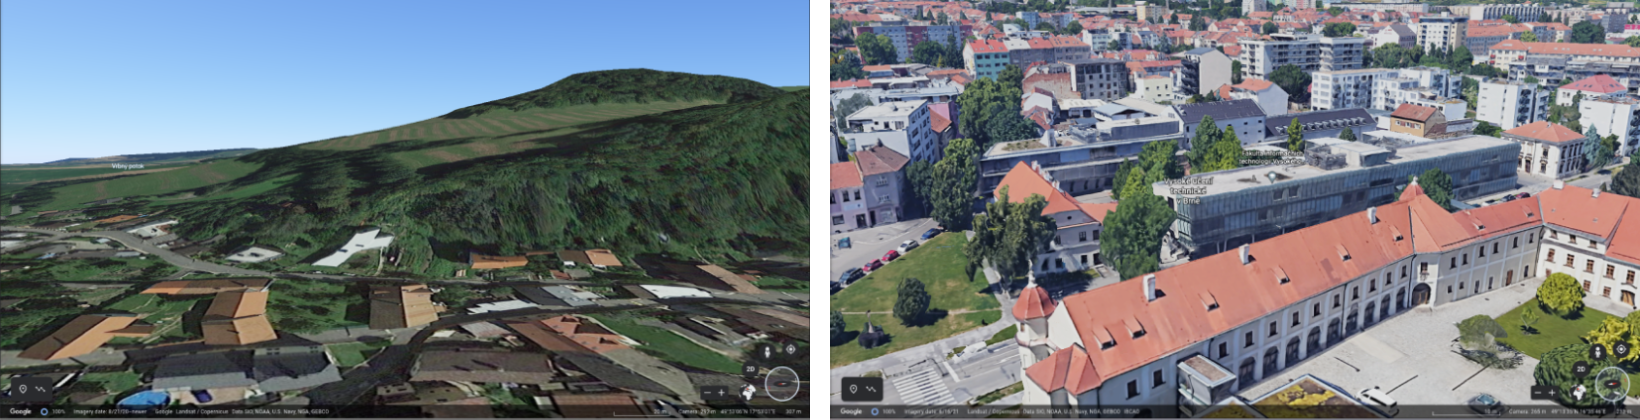
\includegraphics[width=40em]{images/google_earth_comp.png}
	\caption[caption]{Porovnání detailů vesnice (vlevo) a města (vpravo) na Google Earth.} 
	\label{google_earth_comp}
\end{figure}

Mimo jiné má Google Earth i svoje vlastní rozhraní, které je součástí Google Maps API. Nabízí oproti 2D mapám funkce pro 3D. Má tedy stejný ceník a podmínky používání.

\subsection*{Esri ArcGIS}
ArcGIS je sbírka produktů nabízející 2D a 3D mapové podklady. Obsahuje metody, kterými si uživatel může sám vytvořit vlastní mapy. Má funkce na skládání dat z~různých podkladů, vizualizaci vlastních mapových dat, nebo knihovnu pro jazyk Python, ve které uživatelé mohou zpracovávat data.
Základní formou je desktopový klient fungující na všech hlavních platformách, ale existuje i online varianta.

\section{Metody zvyšování kvality modelu} \label{tess-upscale}
Pro realistické zobrazení scény je nutné, aby byly modely ve scéně v~dostatečně vysokém rozlišení. Když je rozlišení moc nízké, začne docházet k~tomu, že mezi jednotlivými polygony jdou vidět tvrdé přechody. Tomu se dá předejít použitím detailnějšího modelu, ale když model s~lepšími detaily není k~dispozici (ať už z~důvodu že se šetří paměť, nebo jednoduše prostě neexistuje), je nutné udělat aproximaci, jak by model mohl vypadat ve vyšším rozlišení. Na to je možné použít několik různých metod, z~nichž nejpoužívanější jsou Curved PN Triangles, Patching Catmull-Clark Meshes a ACC Patches.
\subsection*{Curved PN Triangles}
 Curved PN Triangles\footnote{Curved Point Normal Triangles} je metoda,  která používá rozdělení trojúhelníků na několik menších, čímž prakticky vzniknou nové trojúhelníky, které se vykreslují.
 Tyto nové (menší) trojúhelníky jsou rozmístěny do prostoru podle původních bodů a normálových vektorů těchto bodů. Body jsou rozděleny kubickým způsobem, takže jedna hrana původního trojúhelníku je rozdělena na tři menší, zatímco normálové vektory původních bodů jsou naopak rozděleny kvadratickým způsobem, takže jedna hrana je rozdělena na dvě. Tímto lze dosáhnout dostatečně kvalitní nové geometrie i lepších možnosti stínování, a to bez vytváření zbytečných dat. Obzvláště důležitý je prostřední bod, který je na obrázku \ref{pn_triangle} označen jako b$_{111}$, který dovoluje vypouknutí středu nové geometrie. Informace o~této metodě byly získány z~práce Curved PN triangles \cite{vlachos}.


\begin{figure}[H]
	\centering
	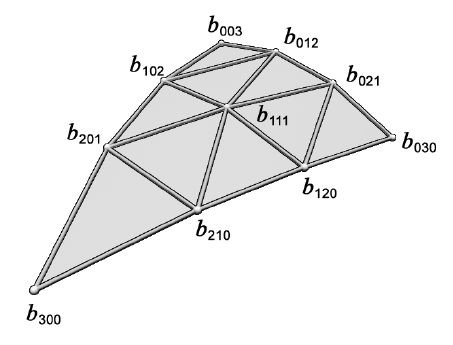
\includegraphics[width=15em]{images/pn/Curved-PN-triangle-tessellation-in-the-graphics-pipeline.png}
	\caption[caption]{Ukázka rozdělení trojúhelníků pomocí techniky Curved PN triangles.\footnotemark }
	\label{pn_triangle}
\end{figure}
\footnotetext{Obrázek převzat z: \cite{vlachos} }

Pokud jsou známé rohové body trojúhelníku $P_{1}, P_{2}, P_{3}$ a jejich normály $N_{1}, N_{2}, N_{3}$, tak lze vypočítat síť zvanou control net, jejíž souřadnice $b_{ijk}\;i,j,k \in \{0,1,2,3\}$ (viz obrázek \ref{pn_triangle}) se získávají následujícím způsobem:
\begin{alignat*}{3}
    b_{300} &= P_{1} \qquad &
    b_{210} &= \frac{(2P_{1} + P_{2} - w_{12}N_{1})}{3} \qquad &
    b_{120} &= \frac{(2P_{2} + P_{1} - w_{21}N_{2})}{3}  \\
    b_{030} &= P_{2} \qquad &
    b_{012} &= \frac{(2P_{3} + P_{2} - w_{32}N_{3})}{3} \qquad &
    b_{021} &= \frac{(2P_{2} + P_{3} - w_{23}N_{2})}{3}  \\
    b_{003} &= P_{3} \qquad &
    b_{102} &= \frac{(2P_{3} + P_{1} - w_{31}N_{3})}{3} \qquad &
    b_{201} &= \frac{(2P_{1} + P_{3} - w_{13}N_{1})}{3} \\
    && b_{111} &= \frac{E + (E - V)}{2} \\
\end{alignat*}
\begin{align*}
     w_{ij} &= (P_{j} - P{i}) \cdot N_{i}\: \: 
    \textit{kde $\cdot$ značí skalární součin} \nonumber  \\
    E &= (b_{210} + b_{120} + b_{021} + b_{012} + b_{102} + b_{201})/6 \nonumber \\
    V~&= (P_{1} + P_{2} + P_{3}) / 3 \nonumber 
\end{align*}

Následně jsou každému takovému nově vygenerovanému bodu v~síti přiřazeny hodnoty $u ,v, w$. Tyto hodnoty jsou v~rozmezí od 0 do 1, a symbolizují hodnotu nového bodu podle barycentrických koordinátů na své Béziér ploše. Z~těchto bodů je pak možné vypočítat body nových trojúhelníků tímto způsobem:
\begin{align}
b(u,v) &= \sum_{i+j+k=3} \frac{3!}{i!j!k!}u^{i}v^{j}w^{k} \nonumber
\end{align}

Také je nutné vypočíst hodnoty normál pro takto vytvořené nové body, a to tak, že se vytvoří síť bodů, které jsou buď lineárně nebo kvadraticky interpolovány. Lineární interpolace narozdíl od kvadratické nebere v~potaz nově vytvořené zakřivení mezi jednotlivými body, jak je ukázáno na obrázku \ref{pn_normal_comparison}. Jednodušší na implementaci je lineární interpolace, ale díky nižší přesnosti se většinou využívá kvadratické.

\begin{figure}[H]
	\centering
	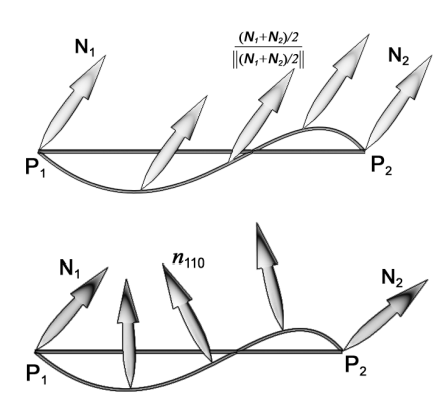
\includegraphics[width=15em]{images/pn/pn-triangle-linear-quad-normals.png}
	\caption[caption]{Porovnání lineárního (nahoře) a kvadratického (dole) výpočtu normál. Šipky značí směr normálního vektoru.\footnotemark}
	\label{pn_normal_comparison}
\end{figure}
\footnotetext{Obrázek převzat z: \cite{vlachos}}

\begin{figure}[H]
	\centering
	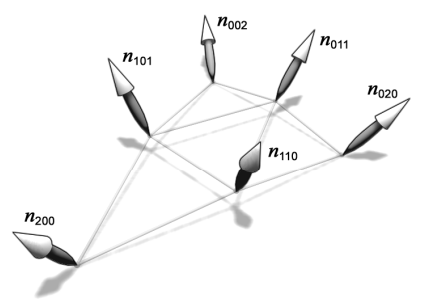
\includegraphics[width=15em]{images/pn/pn-normals.png}
	\caption[caption]{Ukázka kvadratického rozdělení normál na celém trojúhelníku.\footnotemark}
	\label{pn_normal}
\end{figure}

\footnotetext{Obrázek převzat z: \cite{vlachos}}


Výpočet hodnot normál $n_{i,j,k},\:i,j,k \in \{0,1,2\}$ pro jednotlivé body na obrázku \ref{pn_normal} kvadratickou metodou je definován takto:

\begin{alignat*}{3}
    n_{200} &= n_{1} \qquad &        
    n_{110} &= \frac{h_{110}}{\|h_{110}\|} \qquad & 
    h_{110} &= N_{1} + N_{2} + v_{12}(P_{2} - P_{1}) \\
    n_{020} &= n_{2} \qquad &    
    n_{011} &= \frac{h_{011}}{\|h_{011}\|} \qquad &
    h_{011} &= N_{2} + N_{3} + v_{23}(P_{3} - P_{2}) \\
    n_{002} &= n_{3} \qquad & 
    n_{101} &= \frac{h_{101}}{\|h_{101}\|} \qquad &
    h_{101} &= N_{3} + N_{1} + v_{31}(P_{1} - P_{3}) \\
    && && v_{ij} &= 2\frac{(P_{j} - P_{i}) \cdot (P_{i} + P_{j})}{(P_{j} - P_{i}) \cdot(P_{j} - P_{i})}
\end{alignat*}
Normály pro body nově vytvořeného trojúhelníku jsou definovány následovně: 

\begin{align}
    n(u,v) &= \sum_{i+j+k=2} n_{ijk} u^{i}v^{j}w^{k} \nonumber
\end{align}

\subsection*{Patching Catmull-Clark Meshes}
Narozdíl od metody PN Triangles se tato metoda zabývá rozdělováním čtverců. Ty jsou rozděleny bikubickým způsobem, takže z~jednoho čtverce vznikají 4 nové, a při vytváření se bere v~potaz i okolí původních bodů. Při výpočtu nové geometrie tedy nejsou využívány normálové vektory, ale pouze pozice bodů. Metoda vytváří NURBS\footnote{non-uniform rational basis spline} plochy.  Jedná se o~plochu tvořenou body, které mají nějakou pozici a váhu a podle toho je vypočteno zaoblení plochy. Touto metodou je možné získat plochy s~hladkými přechody na všech částech dělené plochy, vyjma okrajů, na kterých je nedostatek informací (právě proto, že nemají okolní body). Zdrojem této metody je \cite{pccm-florida}.

\begin{figure}[H]
	\centering
	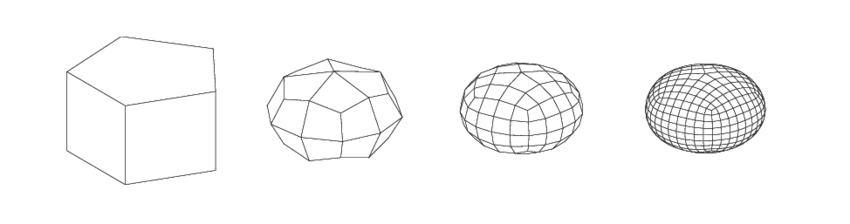
\includegraphics[width=40em]{images/pccm/Three-steps-of-Catmull-Clark-subdivision.png}
	\caption[caption]{Ukázka rozdělení modelu na detailnější pomocí metody PCCM.\footnotemark} 
	\label{pccm_comp}
\end{figure}
\footnotetext{Obrázek převzat z~\cite{pccm-florida}}

Metoda se dá na stejný objekt volat opakovaně a model je tak rozdělován a aproximován stále silněji. Toto je možné vidět na obrázku \ref{pccm_comp}.

\subsection*{ACC Patches}
Metoda ACC Patches\footnote{Approximating Catmull-Clark Subdivision Surfaces with Bicubic Patches} je kombinací výše popsaných metod. Informace o~ní jsou čerpány z~\cite{acc-patches}. Oproti metodě Patching Catmull-Clark Meshes je méně náročná na výpočty, protože ji pouze aproximuje. Pro každý čtverec geometrie je vytvořena plocha s~novou geometrií (geometry patch), a dvě plochy složeny z~tečen (tangent patch), podle kterých jsou určeny normály. Jak už bylo zmíněno, původní metoda nevytváří hladké přechody u~okrajů. ACC Patches toto řeší pomocí použití pole tečen, podle jejichž hodnoty se počítají normály nového povrchu. Metoda také vyžaduje méně větvění, takže je vhodnější pro výpočty a má lepší podporu pro SIMD. 

\section{Metody Ambient Oclusion}
Ambient Oclusion (AO) je technika nasvětlení scény, která aproximuje množství světla dosahující na určitý povrch podle přímo viditelných dalších povrchů v~jeho okolí. Používá se k~tomu, aby scéně přidala jemné stíny, které připomínají  globální iluminaci v~místech jako například rohy místnosti. Zde nemusí dopadat klasické stíny, ale je zde méně světla. Standartní AO je velmi pomalý proces. Pro každý bod se vyšle několik paprsků z~polokoule (ta je sestrojena v~okolí bodu), pomocí kterých se zjistí tvar okolní geometrie. Používá se tedy hlavně v~aplikacích, kde není kladen důraz na vysoký výkon.
V~kontextu této práce je AO důležité pro přidání reálnějšího zobrazení ať už generované vegetace, budov, nebo povrchu samotného.


\subsection*{Screen Space Ambient Oclusion} \label{ssao-theory}
SSAO používá k~zjištění informací o~okolí hloubkový buffer, do kterého jsou zapisovány informace o~fragmentech geometrie při jejím renderování, a poté jsou z~něj čteny vzorky s~informacemi o~okolí.
Pro SSAO algoritmus jsou potřeba dva průchody. V~prvním jsou vygenerovány textury, které jsou později použity pro výpočet AO. V~druhém kroku je vyrenderována samotná scéna, na kterou se přidá SSAO. Vygenerované textury potřebné pro výpočet SSAO jsou následující:
\begin{itemize} \label{ssaotextures}
  \item \textbf{SSAO Depth Texture} -- textura, do které se zapisuje hloubkový buffer scény
  \item \textbf{SSAO Normal Texture} -- textura, do které se zapisuje normálový buffer scény
  \item \textbf{SSAO Random Texture} -- textura, do které se zapisuje náhodný šum
  \item \textbf{SSAO Texture} -- textura, do které se zapisuje výsledek SSAO
\end{itemize}

Pro každý fragment se provede výpočet SSAO funkce. Pomocí vzorkování okolních fragmentů se zjistí tvar okolní geometrie z~Depth Texture. Jaké fragmenty jsou vzorkovány je zjištěno z~Random Texture. Následně se vypočítají rozdíly v~hloubce aktuálního fragmentu, a všech vzorkovaných okolních fragmentů. Tyto hodnoty jsou normalizovány pomocí maximální hloubky okluze. Následně se vyvzorkované hodnoty zprůměrují, a výsledek je faktor okluze. Takto získaná hodnota generuje relativně vysoký šum jak je vidět na obrázku \ref{ssao_noise}.

\begin{figure}[H]
	\centering
	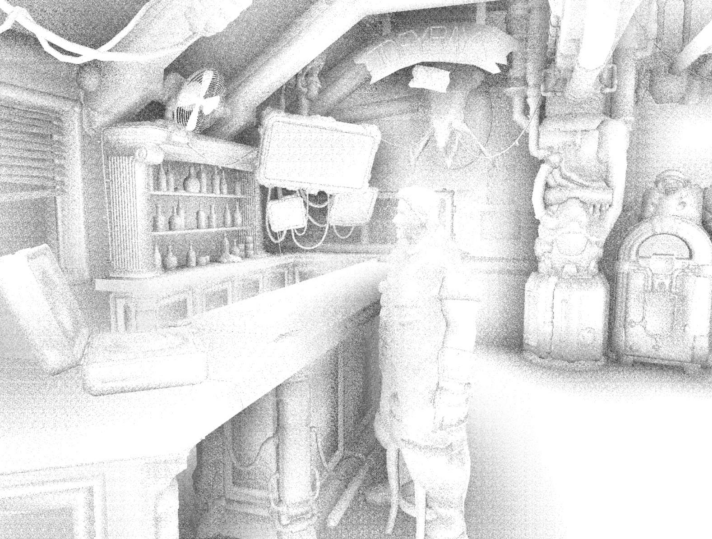
\includegraphics[width=20em]{images/ssao/noise.png}
	\caption[caption]{Ukázka SSAO na scéně ze hry Starcraft II (náhodný šum).\footnotemark} 
	\label{ssao_noise}
\end{figure}

\footnotetext{Obrázek převzat z: \href{https://developer.amd.com/wordpress/media/2013/01/Chapter05-Filion-StarCraftII.pdf}{https://developer.amd.com/wordpress/media/2013/01/Chapter05-Filion-StarCraftII.pdf}}
\label{ssao_noise_text}Tento šum je možné odstranit pomocí funkce na rozmazávání obrazu, například upraveným filtrem \textbf{Gaussian Blur}. Tento filtr se musí upravit tak, aby se nezávislé objekty vzájemně po rozmazání neovlivnily. Na to se použijí Depth Texture a Normal Texture, které jsou vzorkovány v~okolí rozmazávaného bodu. Pokud je okolní hloubka moc vysoká, nebo je skalární součin hodnoty normály bodu a hloubky moc malý, tak je výsledek nahrazen hodnotou 0. Šum je možné aplikovat několikrát, aby se scéna vyhladila co nejlépe. Alternativním způsobem aplikací šumu je vybrat několik okolních pixelů a jednoduše je vyprůměrovat, ale to způsobí, že efekt vypadá mírně rozmazaně. Zdrojem informací o~této metodě je \cite{learnogl}.

\subsection*{Horizon Based Ambient Oclusion}
Horizon Based Ambient Oclusion (HBAO) je metoda, která dosahuje přesných výsledků za cenu poměrně vyššího času zpracování. Je to fyzikálně založený algoritmus, jehož princip je takový, že aproximuje integrál pomocí vzorkování hloubkového bufferu scény. Na určitém povrchu, jsou měřeny jisté úhly, pomocí kterých se zjistí, jak silná bude míra světelné okluze. V~potaz se bere nejen vzdálenost (hloubka), ale i směr normálových vektorů povrchu oproti světu (horizontu). Počítá se tedy i se směrem povrchu, díky čemuž se dají získat přesnější výsledky. Časová náročnost algoritmu způsobí, že je efekt většinou renderován v~nižším rozlišení, a kvůli tomu vznikají určité renderovací artefakty. Ty se dají řešit pomocí postupného filtrování dat a následného odstranění  šumu pomocí rozmazání obrazu podobně jako u~SSAO, viz \ref{ssao_noise_text}. Zdrojem těchto informací je \cite{hbao}.


\begin{figure}[H]
	\centering
	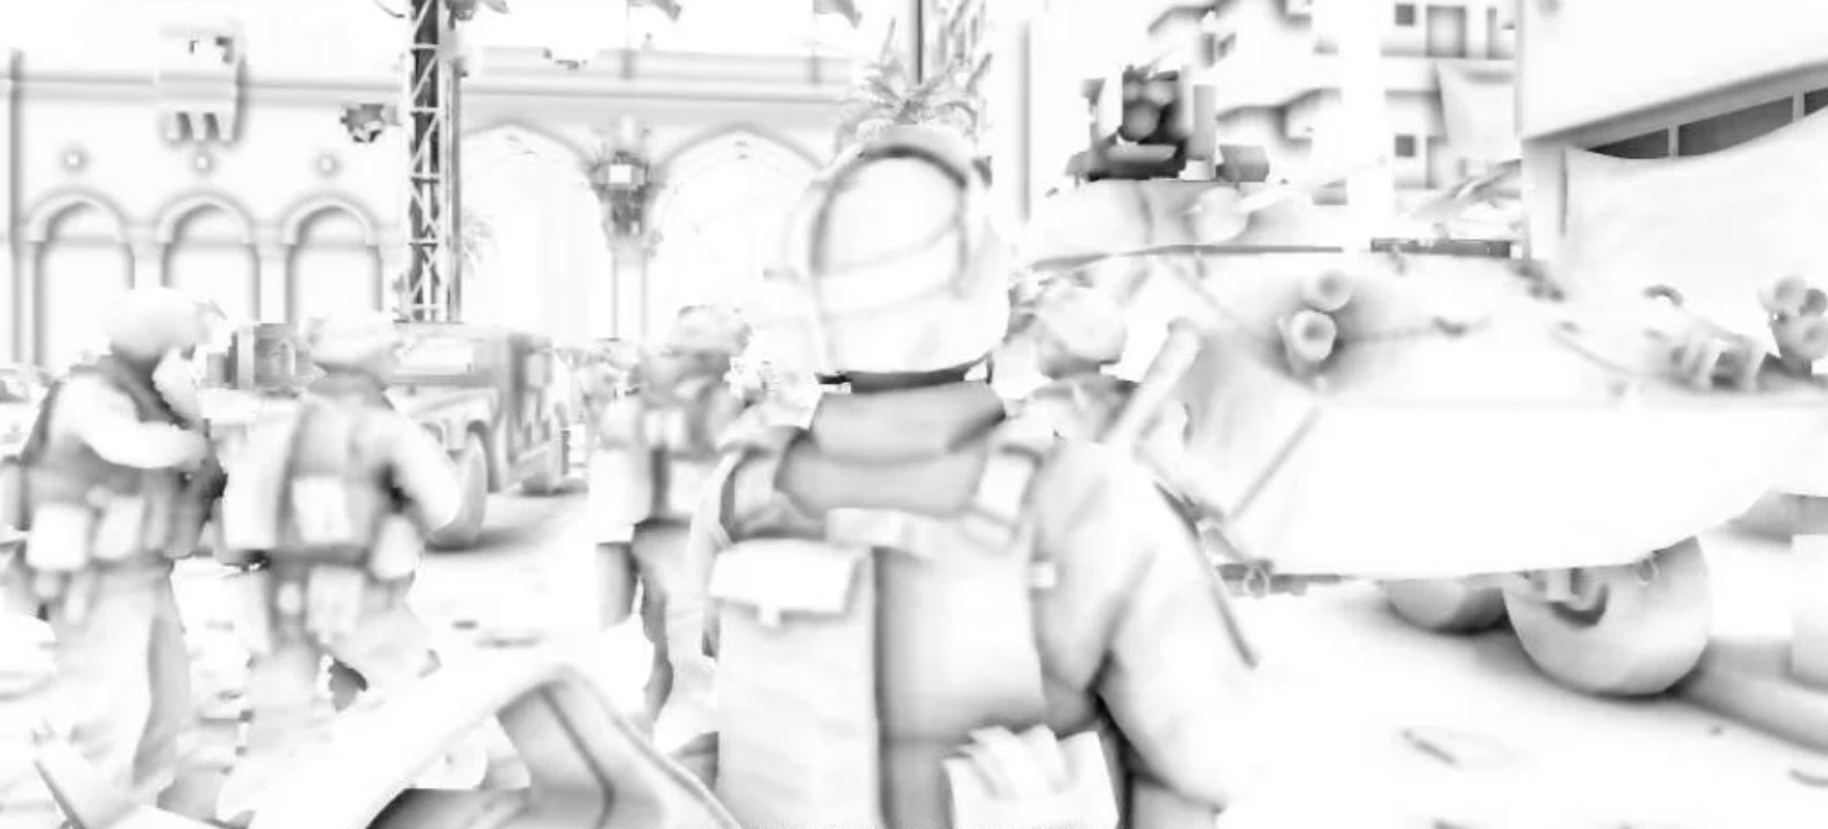
\includegraphics[width=24em]{images/ao/hbao.png}
	\caption[caption]{Ukázka HBAO ze hry Battlefield 3. Na obrázku je zobrazen pouze HBAO průchod scénou.\footnotemark} 
	\label{hbao_example}
\end{figure}

\footnotetext{Obrázek převzat z: \href{https://developer.nvidia.com/sites/default/files/akamai/gamedev/files/gdc12/GDC12_Bavoil_Stable_SSAO_In_BF3_With_STF.pdf}{https://developer.nvidia.com/sites/default/files/akamai/gamedev/files/gdc12/
GDC12\_Bavoil\_Stable\_SSAO\_In\_BF3\_With\_STF.pdf}}
Na obrázku \ref{hbao_example} je ukázka jak vypadá pouze tento efekt v~praxi. Rozšířením této metody je metoda HBAO+, která je přesnější oproti HBAO a dokonce řeší problémy s~výkonem.

\section{Triangulace polygonu} \label{cdt-theory}
Pro vykreslování budov je nejdříve potřeba budovy převést na trojúhelníky tak, aby je bylo možné vykreslit na grafické kartě. To je nutné z~toho důvodu, že budovy mají v~reálném světě tvar polygonu o~$n$ hranách. Jedním z~algoritmů pro triangulaci je Constrained Delaunay Triangulation (CDT). Je to rozšíření algoritmu Delaunay Trinagulation, který neumí pracovat s~konkávními tvary. Tento algoritmus to umí, ale vstupem je kromě jednotlivých bodů také seznam hran (constrained edge -- omezující hrana), popisující, jak má výsledný objekt vypadat. 

\subsection*{Delaunay Triangulation}
Proces generování Deaunay Triangulation má několik možných algoritmů. Nejrychlejší metodou\footnote{\href{https://en.wikipedia.org/wiki/Delaunay_triangulation\#Divide_and_conquer}{https://en.wikipedia.org/wiki/Delaunay\_triangulation}} je \verb|divide and conquer|, která triangulaci vypočítá v~čase $O(n*log(n))$. Ta funguje dle \cite{delaunay} následovně:
\begin{enumerate}[label*=\arabic*.]
    \item Všechny body jsou seřazeny podle jejich koordinátů x. V~případě, že jsou dva koordináty x stejné, jsou seřezeny podle bodu y.
    \item Seznam bodů je postupně rozdělován na poloviny, dokud nejsou v~polovinách dva, nebo tři body. Ze dvou bodů se vytvoří segment, ze tří přímo trojúhelník.
    \item Jednotlivé poloviny bodů jsou rekurzivně spojeny s~druhou polovinou, a výsledkem je triangulace, která se skládá z~několika typů hran: LL -- bod je z~levé triangulace a konec má také v~levé triangulaci; LR -- bod je z~levé triangulace a konec má v~pravé; RR -- začátek i konec jsou v~pravé triangulaci. Při spojování těchto polovin bodů jsou vytvářeny LR hrany. Spojení polovin se dělá následovně:
    \begin{enumerate}[label*=\arabic*.]
        \item Vloží se základní LR hrana, která spojuje nejnižší body triangulací tak, aby neprotínala žádnou LL ani RR hranu.
    \item Je třeba vytvořit další hranu nad touto nově vytvořenou hranou. Na to se musí zvolit další bod, buď z~levé, nebo pravé triangulace, který bude spojen s~jedním z~původních bodů nové hrany. Potencionální body na spojení jsou vybrány v~pořadí velikosti úhlu mezi hranou vytvořenou v~bodě 3.1 a jednotlivými body v~této polovině. Každý z~těchto bodů je zkontrolován dvěmi pravidly. Prvním pravidlem je, že úhel mezi body musí být menší než 180°. Druhým pravidlem je, že opsaná kružnice okolo dvou bodů původní LR hrany a aktuálního potencionálního bodu nesmí obsahovat další potencionální bod. Výběr je zobrazen na obrázku \ref{delaunay-triang-select}.
        \begin{figure}[H]
	\centering
	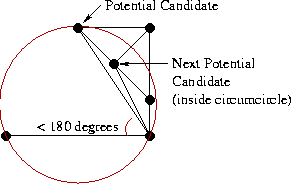
\includegraphics[width=16em]{images/triangulation/bad_pot_cand.png}
	\caption[caption]{Výběr potencionálního kandidáta pro spojení dvou polovin.\footnotemark}
	\label{delaunay-triang-select}
\end{figure}
\footnotetext{Obrázek byl převzat z:  \href{http://www.geom.uiuc.edu/~samuelp/del_project.html}{http://www.geom.uiuc.edu/~samuelp/del\_project.html}}
        \item Pokud jsou obě podmínky splněny, je vybrán první kandidátní bod. Pokud není první podmínka splněna, musí být vybrán bod z~druhé poloviny. Pokud není splněna druhá podmínka, je odebrána RR hrana mezi kandidátním bodem a původním pravým bodem. Tento proces je opakován se všemi body, dokud není vybrán kandidát, nebo se nepočítá s~druhou stranou.
        \item Pokud na pravé straně nebyl žádný kandidát vybrán, proběhne výběr pro levou stranu stejným způsobem.
        \item Když není z~pravé ani levé poloviny získán žádný bod, spojení je kompletní a pokračuje se dalšími polovinami. V~případě, že je získán jen jeden bod, znamená to, že je automaticky spojen, a přeskočí se na krok 3.7. V~případě, že jsou získány body z~obou stran, provede se test, podle kterého bude bod vybrán.
        \item Tento test je následující: pokud pravý kandidátní bod není v~kruhu okolo původní LR hrany a levého kandidátního bodu, je vybrán levý bod a naopak. Této podmínce bude vždy vyhovovat právě jeden z~bodů. Pro představu je výběr zobrazen na obrázku \ref{delaunay-triang-final}.
\begin{figure}[H]
	\centering
	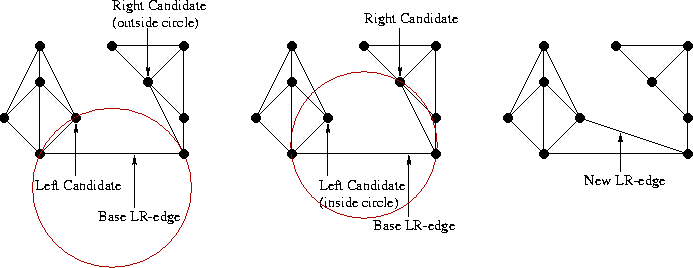
\includegraphics[width=30em]{images/triangulation/cand_final.png}
	\caption[caption]{Test jestli bude vybrán levý nebo pravý kandidátní bod. Na obrázku byl vybrán levý, protože vyhovuje podmínce.\footnotemark}
	\label{delaunay-triang-final}
\end{figure}
\footnotetext{Obrázek byl převzat z:  \href{http://www.geom.uiuc.edu/~samuelp/del_project.html}{http://www.geom.uiuc.edu/~samuelp/del\_project.html}}
        \item Jakmile jsou body propojeny a je vytvořena nová LR hrana, propojování pokračuje s~dalšími hranami s~tím, že za původní hranu se považuje nově vytvořená hrana.
    \end{enumerate}
    \item Poté, co jsou spojeny i poslední dvě poloviny, je triangulace dokončena.
\end{enumerate}\


\subsection*{Constrained Delaunay Triangulation}
Existuje řada algoritmů pro sestrojení trojúhelníku z~polygonu pomocí metody CDT, pro ilustraci je uvedena jedna z~jeho variant, pro kterou bylo čerpáno z~\cite{cdt-book} a \cite{cdt}:

\begin{enumerate}[label*=\arabic*.]
    \item Proběhne iterace přes všechny omezující hrany, které jsou definovány body $V_i$ a $V_j$. Pro každou takovou tu hranu budou provedeny kroky 2-4.
    \item Pokud je omezující hrana $V_i-V_j$ již přítomná, pokračuje se další hranou. Jinak se ve vytvořené triangulaci vyhledají všechny hrany, které prochází touto hranou, a nad nimi se provádí krok 3.
    \item Pro všechny hrany procházející hranou $V_i-V_j$ provádíme následující kroky:
    \begin{enumerate}[label*=\arabic*.]
        \item Hrana je odebrána ze seznamu hran, které procházejí $V_i-V_j$. Tato hrana je definovaná body $V_k$ a $V_l$.
        \item Tato hrana definuje ve vytvořené triangulaci dva trojúhelníky. Pokud tyto dva trojúhelníky netvoří čtyřúhelník, který je konvexní, je hrana umístěna zpět do seznamu hran, a algoritmus se vrací k~bodu 3.1. Jinak proběhne prohození diagonály tohoto čtyřúhelníku. Prohození diagonály je znázorněno na obrázku \ref{cdt-flip-img}. Tato nová diagonála je definována body $V_m$ a $V_n$. Pokud $V_k-V_l$ stále protíná hranu $V_i-V_j$, pak je hrana umístěna do seznamu protínajících hran. Pokud hranu neprotíná, je vložena do seznamu vytvořených hran.
        \begin{figure}[H]
	\centering
	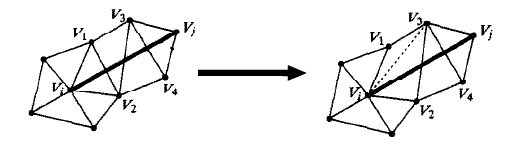
\includegraphics[width=30em]{images/triangulation/cdt.png}
	\caption[caption]{Otočení diagonální hrany $V_1-V_2$ za $V_j-V_3$. Na obrázku body $V_i$ a $V_j$ značí omezující hranu.\footnotemark}
	\label{cdt-flip-img}
\end{figure}
\footnotetext{Obrázek byl převzat a upraven z: \cite{cdt}}
    \end{enumerate}
    \item Dokud dochází k~prohození hran v~kroku 4.3, provádí se následující kroky:
    \begin{enumerate}[label*=\arabic*.]
        \item Probíhá iterace přes všechny hrany ze seznamu nově vytovřených hran.
        \item Nově vytovřená hrana je definována pomocí bodů $V_k-V_l$. Pokud se nová hrana rovná hraně $V_i-V_j$, vrátíme se ke kroku 4.1
        \item Pokud jsou dva trojúhelníky tvořené hranou $V_k-V_l$ umístěny tak, že jeden z~trojúhelníků je uvnitř opsaného kruhu druhého trojúhelníku, potom tyto trojúhelníky tvoří čtyřúhelník s~diagonálou, která stále protíná hranu $V_i-V_j$. V~tom případě je hrana $V_k-V_l$ nahrazena druhou diagonálou tohoto čtyřúhelníku se jménem $V_m-V_n$. Tímto jsou nahrazeny tyto dva trojúhelníky za dva nové trojúhelníky, a hrana $V_k-V_l$ je nahrazena za $V_m-V_n$ v~seznamu nových hran.
    \end{enumerate}
    \item Odeberou se všechny trojúhelníky, které leží mimo supertriangle, což je takový trojúhelník, který opisuje všechny původní body před triangulací.
\end{enumerate}



\section{Procedurální generování vegetace}
Aby bylo dosaženo více realistického zobrazení scény, je třeba vygenerovat vegetaci - stromy v~lese, trávu na loukách a zahradách, obilí na polích. Pozice, kam může být vegetace rozmístěna, se dá spočítat několika způsoby, z~nichž je několik popsáno v~následujících kapitolách.
Poznatky použity v~následujících sekci byly získány z~\cite{melnychuk_2020} a z~\cite{biagioli_2014}.
\subsection*{Náhodné rozložení}
Při náhodném rozložení je vytvořena textura, do které se pomocí libovolné pseudonáhodné funkce od 0 do 1 zapíší hodnoty. Tato textura se poté celá projde, a na každé místo, kde je hodnota textury vyšší než libovolná hodnota $x$, je umístěn nějaký typ vegetace. Tato metoda je výpočetně velmi jednoduchá, ale je s~ní spojena řada problémů. Vegetace nevypadá realisticky (v~reálném světě není vegetace umístěna plně náhodně), a může se stát to, že se kusy vegetace budou protínat, protože jsou moc blízko u~sebe.

\begin{figure}[H]
	\centering
	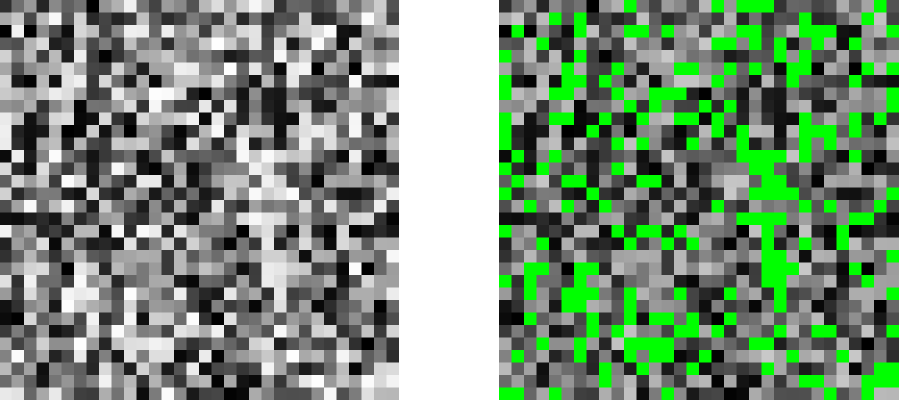
\includegraphics[width=20em]{images/generation/noise.png}
	\caption[caption]{Ukázka rozdělení pomocí náhodného šumu. Vlevo je zobrazen šum samotný a vpravo pozice vegetace v~šumu} 
	\label{rand_noise}
\end{figure}
Na obrázku \ref{rand_noise} jde vidět jak vypadá takové rozdělení v~nižším rozlišení 32x32. Světle zelená barva značí pozice stromů, kde hodnota $x$ byla zvolena přibližně $0.78$. Stromy jsou zde moc blízko u~sebe a nevypadají přirozeně. To se dá řešit tak, že pokud by dva stromy byly moc blízko sebe, jeden se odstraní. To ale stále vede k~nerealistickému zobrazení. 

\subsection*{Rozložení pomocí Perlinova šumu}
Perlinův šum je typ šumu, který se v~3D grafice běžně využívá na generování celé řady efektů jako plameny ohně, kouř, oblaka, nebo také realisticky vypadající procedurálně generované terény, či planety. Svou popularitu získal díky jednoduché a rychlé implementaci a vysoké realističnosti při procedurálním generování. Většinou je skládáno více vrstev šumu dohromady, aby se dosáhlo realističtějšího zobrazení. Pro generování vegetace je možné Perlinův šum využít podobně jako obyčejného šumu. Musí se zde také řešit překrývání vegetace. Generování probíhá takovým způsobem, že je vybrána hodnota z~šumu, a jestli je vyšší než vybraná hodnota $x$, tak je zde umístěna vegetace. Použítí Perlinova šumu vede k~skupinám vegetace, které mají vysokou hustotu, a skupinám, které mají naopak hustotu nízkou. Tohoto je využíváno například ve hrách, kdy se tyto velké plochy stromů využijí pro oddělení herních oblastí, a hráč pak přes les neprojde.
\begin{figure}[H]
	\centering
	
\includegraphics[width=20em]{images/generation/perlin_noise.png}
	\caption[caption]{Ukázka rozdělení pomocí Perlinova šumu. Vlevo je zobrazen šum samotný a vpravo pozice vegetace v~šumu} 
	\label{perlin_noise}
\end{figure}
Na obrázku \ref{perlin_noise} je vidět, jak by se vygenerovala vegetace s~poušitím Perlinova šumu s~hodnotou $x$ nastavenou na $0.58$.

\subsection*{Rozložení s~užitím celulárních automatů}
Další možností je využití celulárních automatů. Buňky automatu můžou mít stavy 1, nebo 0, které označují, jestli na bodě je, nebo není vegetace. Musí být určen počáteční stav automatu, přičemž je možné jej nastavit náhodně. Automat běží několik iterací tak, aby bylo docíleno co nejlepšího výsledku. Tímto způsobem vzniká vegetace, která má velmi realistické rozložení. Hlavní problém je, že vegetace je umístěna do mřížky podle toho, jak byl vytvořen automat. To se dá řešit tak, že se každý prvek vegetace posune, avšak výsledky pak vypadají méně opět méně realisticky, a stále není vyřešeno překrývání.
\begin{figure}[H]
	\centering
	
\includegraphics[width=12em]{images/generation/cellular.png}
	\caption[caption]{Ukázka rozdělení pomocí celulárních automatů. \footnotemark}
	\label{cellular_vegetation}
\end{figure}

\footnotetext{Obrázek převzat z: \cite{melnychuk_2020}.}

Obrázek \ref{cellular_vegetation} je ukázkou jak může vypadat vegetace po rozdělení s~užitím celulárních automatů.

\subsection*{Poisson disk sampling} \label{poisson_sampling}
Další metodou je Poisson disk sampling. Ta povoluje generovat body v~$n$ dimenzionálním prostoru a zajišťuje, že body budou vygenerovány s~určitou vzdáleností od sebe, takže se výsledně generovaná vegetace nepřekrývá. Vstupem algoritmu je vzdálenost $r$ mezi body, velikost generovaného prostoru a počet pokusů $k$. Hodnota $k$ určuje maximální počet neúspěšných pokusů o~vytvoření nového bodu. Jakmile algoritmus provede pro daný bod tento počet pokusů, přesune se na jinou pozici. Body jsou pak vygenenrovány pomocí následujícího algoritmu:
\begin{enumerate}
  \item Vypočte se velikost buňky $c = \frac{r}{\sqrt{n}}$.
  \item Vytvoří se $n$ rozměrná mřížka s~délkou hrany $\frac{max}{c}$, kde $max$ značí maximální rozlišení mřížky s~tím, že délka hrany je zaokrouhlená nahoru k~nejbližšímu celému číslu.
  \item Vytvoří se dva seznamy. Jeden na uložení vytvořených bodů a druhý na vytvoření aktivních bodů. Aktivní body jsou takové body, které mohou ještě mít další nové sousední body.
  \item Vytvoří se první bod, který je umístěn do mřížky a do seznamu aktivních bodů.
  \item Dokud není aktivní seznam prázdný, probíhá iterace přes body $i$ následovně:
  \begin{enumerate}
    \item Vytvoří se nový bod na pozici vypočítané pomocí náhodného směrového vektoru $d$, který lze získat z~náhodného úhlu $\alpha$. $\alpha = x * \pi * 2$, kde $x$ značí náhodnou hodnotu. Pro dvourozměrnou mřížku je vektor $d$ vypočítán tak, že jedna složka je rovna $\sin(\alpha)$ a druhá složka je rovna $\cos(\alpha)$. Nový bod má pak pozici definovanou jako $p = i + d * rand(r, r*2)$, kde $rand(y,z)$ značí funkci generující rovnoměrné rozdělení v~intervalu $<y;z>$.
    \item Proběhne kontrola, zda se body překrývají. Pokud ano, vrátí se algoritmus k~předchozímu bodu, a je odebrán jeden pokus (z~celkových $k$ pokusů).
    \item Pokud byl bod vytvořen, je přidán do aktivního seznamu, a je generován další bod.
    \item Pokud po $k$ pokusech nebyl žádný bod vytvořen, znamená to, že bod $i$ nemůže mít další sousedy, a je tedy odebrán z~aktivního seznamu.
  \end{enumerate}
  \item Pokud již nejsou dostupné žádné nové body, generování je ukončeno.
\end{enumerate}

\begin{figure}[H]
	\centering
	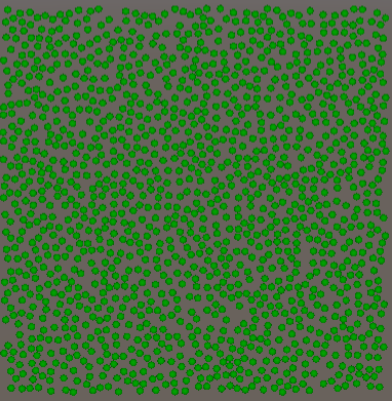
\includegraphics[width=12em]{images/generation/poisson.png}
	\caption[caption]{Ukázka rozdělení pomocí metody Poisson disk sampling.\footnotemark} 
	\label{poisson_vegetation}
\end{figure}
Na obrázku \ref{poisson_vegetation} je ukázáno, jak vypadá výsledné rozdělení vegetace na 2D ploše. Zelené body značí, kam tato metoda umístí vegetaci. Postup pro tuto metodu čerpá z~\cite{poisson-sampling}
\footnotetext{Obrázek převzat z: \cite{melnychuk_2020}.}
\section{Deferred shading}
Klasickým způsobem renderování scény je forward shading. U~této metody je pro každý objekt ve scéně vypočítáno osvětlení tak, že se iteruje přes každý zdroj světla, a objekt je postupně nasvětlen. To je výpočetně velmi náročné, protože komplexnější scény s~více světly musí provést zbytečně vysoké množství iterací. Zároveň když se dva objekty vzájemně překrývají, může se stát, že je část výsledného obrazu několikrát přepočítávána znovu právě díky překrytí objektů. Toto se dá vyřešit pomocí techniky deferred shading. Tato technika je založena na tom, že se odloží zobrazení veškerého nasvícení scény na později. Deferred shading je rozdělen na dvě fáze.

V~první fázi se sesbírají různé informace o~geometrii objektů ve scéně, a ty jsou uloženy do speciálního bufferu s~názvem G-Buffer (geometry buffer). G-Buffer obsahuje několik textur se stejným rozlišením jako výsledný obraz. Do textur jsou uloženy informace o~pozici, normálový vektor, barva \footnote{albedo} a lesklost \footnote{specular} každého pixelu (fragmentu) scény. Lesklost se dá uložit do alpha složky barevné textury, a je tím možno ušetřit jednu texturu a snížit tím paměťovou náročnost metody, která je relativně vysoká. Pro přesnost uložení dat jako pozice a normálové vektory nestačí použít malé datové typy jako byte, ale je třeba větších, které zabírají více paměti. V~případě rozlišení 4K (3840x2160) a využití všech textur se jedná o~téměř 1.6 GB paměti, což je poměrně hodně i na moderní grafické karty. Když se využije deferred shading, je také velmi jednoduché implementovat celou řadu screen space post process efektů. Příkladem takového efektu je metoda SSAO, jejíchž dvě vstupní textury jsou přímým výstupem právě deferred shadingu viz \ref{ssaotextures}. Jak takové textury mohou vypadat je ukázáno na obrázku \ref{g-buffer-images}. 
\begin{figure}[H]
	\centering
	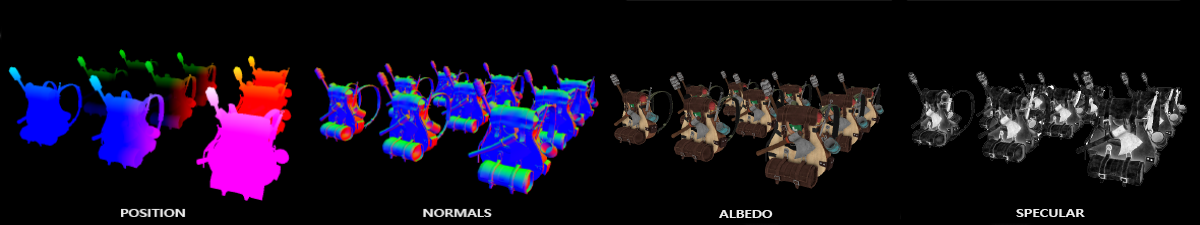
\includegraphics[width=40em]{images/navrh/deferred_g_buffer.png}
	\caption[caption]{Ukázka textur v~G-Bufferu.\footnotemark} 
	\label{g-buffer-images}
\end{figure}
\footnotetext{Obrázek převzat z: \href{https://learnopengl.com/Advanced-Lighting/Deferred-Shading}{https://learnopengl.com/Advanced-Lighting/Deferred-Shading}}

V~druhé fázi deferred shadingu nastane výpočet nasvícení scény. Přes celou obrazovku se zobrazí pouze obdélník, na který se ve fragment shaderu vypočítá výsledná textura reprezentující finální scénu. Iteruje se přes každý pixel v~texturách z~G-bufferu, a je vypočítáno nasvícení světly ve scéně. Tím, že je nasvícení počítáno na texturách, proběhne výpočet pouze jednou pro každý pixel scény. V~případě, že scéna obsahuje větší množství světel a překrývajících se objektů, je díky tomu ušetřeno relativně vysoké množství výkonu. Nasvícení na takovýchto texturách může být počítáno naprosto stejně jako u~klasického forward shadingu, kde je počítáno pro každý objekt zvlášť. Informace v~této sekci byly získány z~\cite{learnogl}.

\begin{figure}[H]
	\centering
	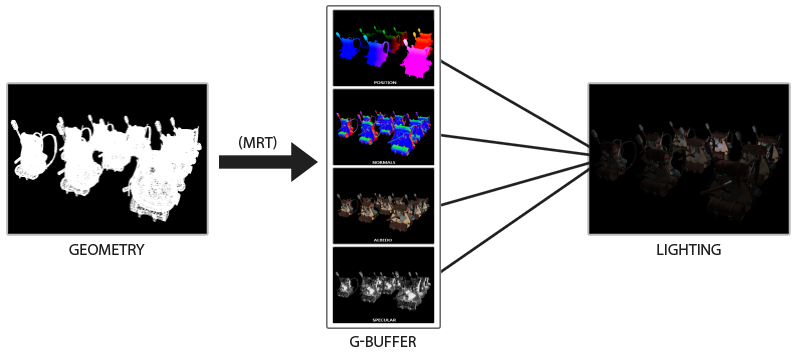
\includegraphics[width=30em]{images/navrh/deferred_overview.png}
	\caption[caption]{Proces deferred shadingu. \footnotemark} 
	\label{g-buffer-overview}
\end{figure}

\footnotetext{Obrázek převzat z: \href{https://learnopengl.com/Advanced-Lighting/Deferred-Shading}{https://learnopengl.com/Advanced-Lighting/Deferred-Shading}}


Na obrázku \ref{g-buffer-overview} je vidět, jak probíhá deferred shading. Geometrie je rozdělena na jednotlivé textury, jsou provedeny výpočty, a výsledky jsou vloženy do výsledné scény včetně nasvícení.



\pagebreak
\chapter{Výběr technologií a návrh funkcionality aplikace}
Tato kapitola popisuje návrh aplikace, který je vytvořen tak, aby aplikace byla co nejvíce přínosná koncovému uživateli. V~případě této aplikace se jedná o~obyčejného člověka, který se chystá na výlet do nějaké oblasti, a chce si tuto oblast vizualizovat v~3D prostoru. Aplikace by tedy měla být jednoduchá na použití i pro někoho, kdo není informatik. 

\section{Architektura aplikace}
Jelikož má být aplikace využívána běžnými uživateli, tak je potřeba, aby byla multiplatformní, a byla přístupná jako desktopová aplikace. Vhodným jazykem pro tuto práci je jazyk C++, protože nabízí framework Qt pro uživatelské rozhraní. Hlavní logika aplikace by měla být samostatná knihovna, která má co nejméně dependencí, a ideálně je i přenosná mezi různými systémy. Samotná spustitelná aplikace je navržena jako pouze frontend volající funkce z~knihovny, a zobrazení výstupu knihovny. Tímto je možné docílit toho, že aplikaci bude jednoduše možné v~budoucnosti zkompilovat i do technologií jako je WebAssembly, a vytvořit z~práce webovou aplikaci.

Vstupem této aplikace budou 2 koordináty na libovolné pozici na zemi ve formátu zeměpisné výšky a šířky. Dohromady tvoří rohy obdélníku okolo oblasti, která bude knihovnou vygenerována. Uživatel tyto koordináty zadá pomocí uživatelského rozhraní, na kterém se zobrazí klasická 2D mapa, a nějakou akcí (například potažením myši) vybere oblast. Poté se získají data pro tuto oblast a započne výpočet. Ten by měl běžet asynchroně a postupně vracet detailnější informace o~oblasti, aby uživatel čekal co nejkratší dobu na minimální možné informace.
Výstupem bude scéna obsahující jednotlivé modely, textury, shadery, další grafické objekty, a popisy, jak se má scéna zobrazit. Součástí výstupu, už ale nebudou postprocess efekty, jako je například SSAO, které nejsou potřebné pro funkčnost, a uživatel knihovny si je dokáže nadefinovat sám. Pro případ této práce bude na zobrazování dat využita knihovna GPUEngine\footnote{https://github.com/Rendering-FIT/GPUEngine}, vyvíjena na VUT FIT, která staví nad grafickým rozhraním OpenGL.

\section{Výběr zvolených technolgií}
Z~výše zmíněných technologií v~sekci \ref{2Dmaps} je třeba zvolit vhodnou technologii pro každou část implementace. Každá má své výhody a nevýhody, podle kterých je posouzena vhodnost použití v~této práci.

\subsection*{API pro mapové podklady}
Jako mapové podklady je možné použít API, které byly zmíněny v~sekci \ref{2Dmaps}. Porovnání jejich vlastností je uvedeno v~tabulkách \ref{table:osm}, \ref{table:gmaps} a \ref{table:bingmaps}.
\begin{itemize}
    \item \textbf{OpenStreetMap} -- Hlavní výhodou je, že data jsou zadávána uživateli. Z~toho plyne, že data jsou velmi přesná (když uživatel vidí někde chybu, může ji sám opravit). Zároveň to ale znamená, že uživatel může zadat i data, které jsou nějakým způsobem nepřesná. Vlastnost, že je služba vedena uživateli, vede také k~tomu, že s~ní pracuje spousta lidí, a existuje tedy rozsáhlá dokumentace a řada uživatelských projektů, které na těchto mapách staví. Drobnou nevýhodou je, že API vrací opravdu velmi detailní údaje. Pro přibližnou oblast města Brna API vrací přes 400MB dat, což na pomalejším internetovém připojení znamená, že uživatel na data musí dlouho čekat. Požadavky se dají zoptimalizovat tak, aby byly pro stejnou oblast přibližně 200MB dat, ale to je stále hodně. Pro představu na průměrném českém internetu v~roce 2020, tj. na přibližně 74 Mbps\footnote{\href{https://www.statista.com/statistics/1155589/internet-connection-speeds-czechia/\#:~:text=As\%20of\%20December\%202020\%2C\%20the,slower\%2C\%20at\%20around\%2061.8\%20Mbps}{https://www.statista.com/statistics/1155589/internet-connection-speeds-czechia/}}, by se data stahovaly okolo 20 sekund. Za tuto dobu uživatel pouze čeká na načtení aplikace.

    \item \textbf{Google Maps} -- Google Maps jsou většinou mírně přesnější než zmíněné OpenStreetMap. Příkladem je například budova blízko místa mého bydliště, která ovšem reálně není budova, ale auto, které tam někdy parkovalo. Na Google mapách jsou data zadána správně. Nevýhodou je, že Google Maps API neobsahuje vhodný endpoint na získání metadat o~oblasti. Jsou zde endpointy na získání statického obrázku, který obsahuje slepou mapu oblasti, a z~té je možné (např. dle barvy) získat informace o~tom, o~jaký typ oblasti se jedná. Zde ale může docházet k~nepřesnostem daným tím, že je aplikace limitována pouze na odhad. Google Maps API obsahuje i několik způsobů jak získat výškové data. Problém ale je, že to je buď získání informací o~jednom bodu, nebo o~čáře mezi dvěma body. V~kontextu této práce to znamená, že by bylo nutné opravdu velmi vysoké množství požadavků aby byly data použitelná. Vhodným využitím API je zobrazování statických 2D map, nebo výškového profilu.

    \item \textbf{Bing Maps} -- Bing Maps nejsou vhodné na získávání metadat o~oblasti -- nemají na to žádné endpointy. Na co jsou Bing Maps velmi dobré, je získávání výškových dat. Krom toho že data jsou velmi přesná, je i přístup k~nim jednoduchý. Jedním požadavkem lze získat až 1024 výškových bodů v~libovolné obdélníkové oblasti. Pro získání výškových dat z~nějaké oblasti je tedy nutné zastlat pouze jeden požadavek obsahující několik ohraničujících koordinátů a API vrátí rovnoměrně rozložené výškové body pro tuto oblast. V~případě větší oblasti (několik km) ale není 1024 bodů z~daleka dostačující. Jedná se o~rozlišení 32x32 bodů a to je velmi málo. Je možné zaslat více požadavků po sobě a následně data poskládat do jedné větší oblasti, ale to také není ideální. Hlavní problém s~tímto přístupem je, že Bing Maps mají nastavený limit na požadavků v~určitém čase. Když je tento limit překročen, je API nedostupné až přes 10 vteřin. Limit není v~dokumentaci zmíněn, ale z~testování vyplynulo, že je to přibližně 16 rychle po sobě poslaných požadavků, ale často i méně. Při 16 požadavcích se jedná o~rozlišení 128x128. Bing Maps API je tedy vhodné limitovat na maximální rozlišení 96x96, které je vždy v~pořádku. V~případě využití tohoto API bude v~práci nutné využít některou z~metod popsaných v~sekci \ref{tess-upscale}.

\end{itemize}

    \begin{table}[h]
    \centering
    \begin{tabular}{| m{18em} | m{18em}|}
    \hline
    \multicolumn{2}{|c|}{\textbf{Google Maps}}                                                \\ \hline
    \multicolumn{1}{|c|}{\textbf{Výhody}}              & \multicolumn{1}{c|}{\textbf{Nevýhody}} \\ \hline
    \multicolumn{1}{|l|}{Přenost a kvalita dostpných dat} & Cena za použití může být vysoká           \\ \hline
    \multicolumn{1}{|l|}{Rychlost} & Dokumentace není ideální    \\ \hline
    \multicolumn{1}{|l|}{}  & Nevhodné endpointy pro tuto práci   \\ \hline
    \end{tabular}
    \caption{Porovnání výhod a nevýhod Google Maps}
    \label{table:gmaps}
    \end{table}

    \begin{table}[h]
    \centering
    \begin{tabular}{| m{18em} | m{18em}|}
    \hline
    \multicolumn{2}{|c|}{\textbf{OpenStreetMap}}                                                \\ \hline
    \multicolumn{1}{|c|}{\textbf{Výhody}}  & \multicolumn{1}{c|}{\textbf{Nevýhody}} \\ \hline
    \multicolumn{1}{|l|}{API je uživatelsky přívětivé} & Data nejsou z~daleka vždy perfektní  \\ \hline
    \multicolumn{1}{|l|}{Data jsou zadavána uživateli} & API vrací velmi vysoké množství dat  \\ \hline
    \multicolumn{1}{|l|}{Spousta dostupné dokumentace}&  \\ \hline
    \multicolumn{1}{|l|}{Zcela zdarma} &     \\ \hline
    \end{tabular}
    \caption{Porovnání výhod a nevýhod OpenStreetMap}
    \label{table:osm}
    \end{table}

    \begin{table}[h]
    \centering
    \begin{tabular}{| m{18em} | m{18em}|}
    \hline
    \multicolumn{2}{|c|}{\textbf{Bing Maps}}   \\ \hline
    \multicolumn{1}{|c|}{\textbf{Výhody}}  & \multicolumn{1}{c|}{\textbf{Nevýhody}} \\ \hline
    \multicolumn{1}{|l|}{Kvalita výškových dat} & Bez možnosti získat metadata          \\ \hline
    \multicolumn{1}{|l|}{Výborná dokumentace}& Velmi tvrdé limity na počet požadavků   \\ \hline
    \multicolumn{1}{|l|}{Rychlost}  &   \\ \hline
    \multicolumn{1}{|l|}{Možnosti získávání výškových dat}  &   \\ \hline
    \end{tabular}
    \caption{Porovnání výhod a nevýhod Bing Maps}
    \label{table:bingmaps}
    \end{table}

Z~výše popsaných výhod a nevýhod plyne, že použítí Google Maps v~práci nebude vhodné, a budou využity Bing Maps pro získání výškových dat a OpenStreetMap pro získání metadat. Obě dvě použité API vrací data ve formátu JSON, který bude do objektu serializován pomocí knihovny \verb|JSON for Modern C++|\footnote{\href{https://github.com/nlohmann/json}{https://github.com/nlohmann/json}}. 
\subsection*{Zvýšení kvality modelů} \label{tess-method-selection}
Jelikož pro plochy, které mají v~reálném světě několik kilometrů čtverečních, je využití výškových podkladů s~rozlišením maximálně 96x96 bodů nevhodné, je třeba povrch zlepšit. Takto malé rozlišení může způsobovat nepřesnosti nebo dalších problémy, které mohou nastat například s~nasvícením scény. To v~práci bude implementováno pomocí jedné z~metod popsaných v~sekci \ref{tess-upscale}. Metoda poběží na grafické kartě tak, aby ušetřila co nejvíce výpočetního výkonu na procesoru, kde by metoda zabrala podstatně více času. Porovnání metod pro zvýšení kvality modelů:


\begin{itemize}
    \item \textbf{Curved PN Triangles} -- Výhoda této metody je, že je relativně jednoduchá na implmentaci jako tessalační shader v~OpenGL. Vytváří ovšem chybu (drobné artefakty) v~geometrii a v~normálách u~některých tvarů objektů. Další výhodou je, že výpočty probíhají na úrovni trojúhelníků, což opět vyhovuje OpenGL, které pracuje při renderu také primárně s~trojúhelníky.
    
    \item \textbf{Patching Catmull-Clark Meshes} -- Hlavní nevýhodou tohoto algoritmu je, že pracuje se čtverci. To v~kontextu práce není problém -- povrch je možné generovat ať už jako čtverce nebo jako trojúhelníky. Problém to je ale při zobrazování povrchu na grafické kartě s~využitím knihovny \verb|OpenGL|, který pracuje primárně s~trojúhelníky. Oproti metodě Curved PN Triangles je ale složitější na implementaci a v~některých případech má vyšší chybovost. Algoritmus je možné implementovat na grafické kartě, ale není k~tomu vhodný z~důvodu nižší rychlosti. 
    
    \item \textbf{ACC Patches} -- Tato metoda má velmi vysokou přesnost -- téměř nevytváří chyby jak v~geometrii tak v~normálách geometrie, ale oproti ostatním metodám má nejsložitější implementaci. Je velmi vhodná na implementaci na grafických kartách a dosahuje i velmi dobré rychlosti -- obzvlášť oproti PCCM metodě, kterou tato metoda aproximuje.
\end{itemize}

Na obrázku \ref{tess-methods-comp} je vidět porovnání chybovosti všech metod, oproti geometrii, která už byla ve vyšším rozlišení.


\begin{figure}[H]
	\centering
	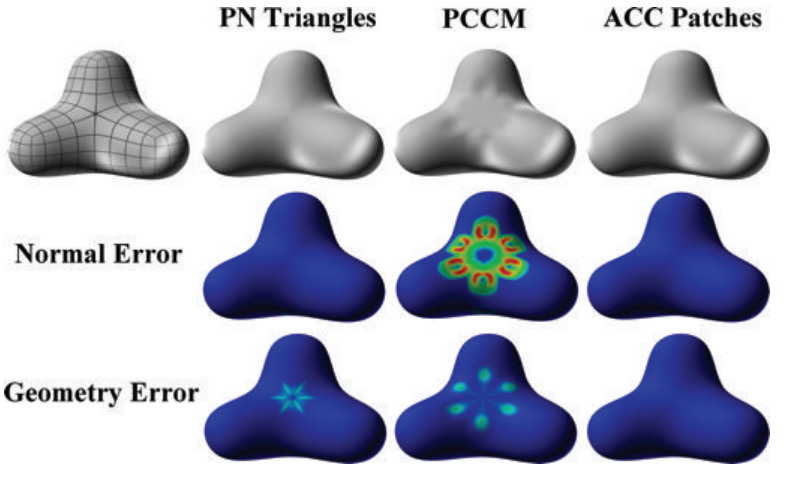
\includegraphics[width=30em]{images/navrh/compare-tess.png}
	\caption[caption]{Porovnání metod zvyšování rozlišení geometrie. Každý z~povrchů byl rozdělen dvakrát, každý jinou metodou. U~PCCM vzniká relativně vysoká chyba normál, narozdíl od ostatních metod.\footnotemark} 
	\label{tess-methods-comp}
\end{figure}
\footnotetext{Obrázek převzan z: \cite{acc-patches}}

V~práci bude použita metoda Curved PN Triangles, která dosahuje dostatečně dobrých výsledků a je jednochá na implementaci.  

\subsection*{Generování vegetace}
Práce bude reprezentovat realistické zobrazení nějaké oblasti ve skutečném světě. Nereálně vypadající zobrazení náhodného rozdělení vegetace je tedy i přes to, že je velmi rychlé na implementaci, nevhodné použít. Rozložení pomocí perlinova šumu generuje reálněji vypadající vegetaci, ale na generování vegetace oproti jiným přístupům je méně realistický, a proto také nebude využit. Rozložení za pomocí celulárních automatů generuje relativně reálně vypadají vegetaci, ale jejich implementace je složitější a výsledky stále nejsou ideální. Zároveň se zde musí řešit řada problémů, jako například překrývání, a fakt, že vegetace je přesně umístěna do mřížky. Pro nejrealističtější zobrazení je proto vhodné použít algoritmus Poisson Disk Sampling \ref{poisson_sampling}, který i sám řeší překrývání vegetace a podobné problémy. 

Ten bude implementován tak, aby příjmal několik různých typů vegetace (např. jehličnaté a listnaté stromy, tráva, obiloviny). Algoritmus bude moct míchat i více různých typů vegetace tak, aby mohly vzniknout i například smíšené lesy. O~každém druhu vegetace bude předem známá informace o~tom, jak daleko od sebe mají být jednotlivé kusy a jak jsou velké. Algoritmus pak zaplní všechny oblasti, kde se má vegetace objevit ve finální reprezentaci světa, a pokud budou nějaké vygenerovány mimo, budou odstraněny. Generování samotných vzorků bude zprostředkováno pomocí knihovny \label{sampling-lib}\verb|poisson-disk-sampling|\footnote{\href{https://github.com/thinks/poisson-disk-sampling}{https://github.com/thinks/poisson-disk-sampling}}, která je zabalená pouze do jednoho hlavičkového souboru, a bude s~ní tedy jednoduché pracovat. Výsledek generování poomocí knihovny je na obrázku \ref{sampling-lib-example}.

\begin{figure}[H]
	\centering
	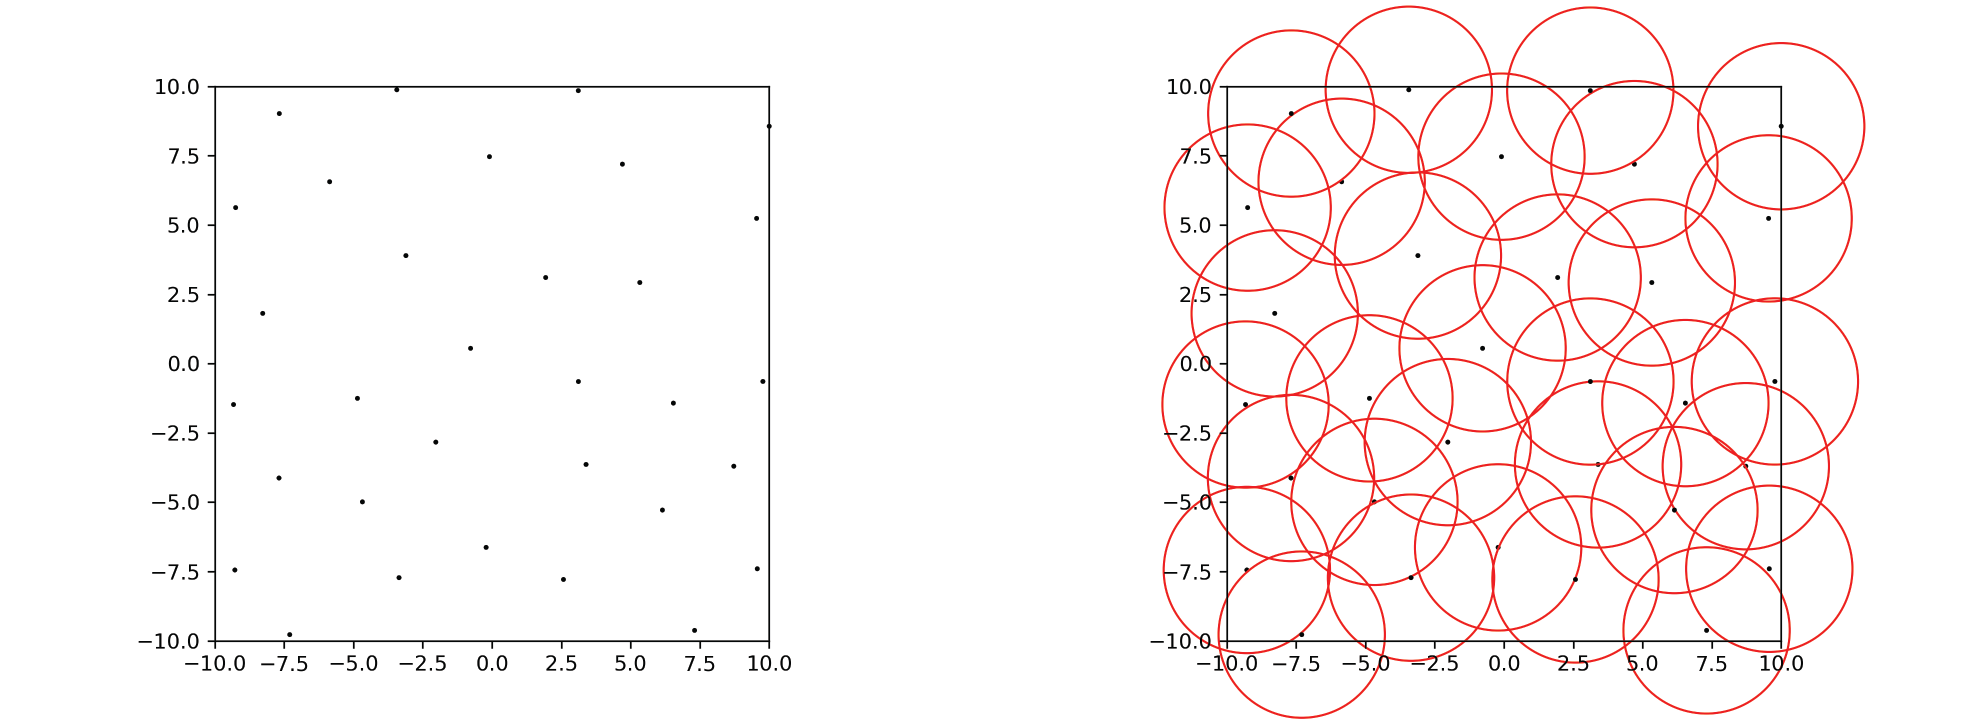
\includegraphics[width=30em]{images/generation/poisson-sampling-example.png}
	\caption[caption]{Ukázka jak knihovna zmíněna zde \ref{sampling-lib} generuje vzorky. Vlevo výsledné body, vpravo body včetně kruhů, zajišťující že se body nepřekrývají.\footnotemark} 
	\label{sampling-lib-example}
\end{figure}

\footnotetext{Obrázek převzat z: \href{https://github.com/thinks/poisson-disk-sampling}{https://github.com/thinks/poisson-disk-sampling}}

Zobrazení vegetace bude probíhat pomocí instanced renderingu, který probíhá tak, že procesor dá instrukci grafické kartě na vykreslení pouze jednou (pro každý typ vegetace), ale předem bude vytvořen buffer, který obsahuje dodatečné informace, jako například offsety a rotace. Offsety říkají, o~kolik se má vegetace posunout oproti základnímu modelu, rotace jsou určeny úhlu, který se má vegetace orotovat, aby bylo zobrazení realističtější a všechny kusy nevypadaly přesně stejně. Tímto se podstatně zvedne výkonnost renderování vegetace. Pro vysoké množství vegetace (přes 150 000 kusů) by bylo nemožné docílit rozumného výkonu klasickým způsobem, kde se každý kus vegetace vykresluje zvlášť, alespoň ne na aktuálním hardwaru.

\subsection*{Generování budov}
Pro generování budov bude v~práci použit algoritmus CDT popsaný v~sekci \ref{cdt-theory}. V~práci bude použita open-source knihovna \verb|CDT|\footnote{\href{https://github.com/artem-ogre/CDT}{https://github.com/artem-ogre/CDT}}. Výstup této knihovny bude využit na seskládání podlahy a jednotlivých střech budovy, přičemž budova může mít různý počet pater. Výška budovy bude určena podle počtu jejích pater. Počet pater se dá u~některých budov získat z~OpenStreetMap API. U~budov, kde není zadán počet pater, bude počet pater nastavený na hodnotu 1. Výška patra bude nastavena na 4.2 metrů, což je přibližně průměrná výška patra, která činí 14 stop\footnote{\href{https://theskydeck.com/how-tall-is-a-storey-in-feet/}{https://theskydeck.com/how-tall-is-a-storey-in-feet/}}. Stěny budovy budou sestrojeny tak, že se projdou původní body reprezentující podlahu a body s~offsetem vysokým podle výšky budovy, a pro každou stěnu mezi těmito body se sestrojí dva trojúhelníky reprezentující tuto stěnu.

\subsection*{Výběr Ambient Oclusion metody}
Jelikož Ambient Oclusion v~reálném čase je na současném hardwaru nereálný, je na výběr buď metoda SSAO nebo HBAO. Jako metoda, která v~aplikaci bude používána, byla zvolena metoda SSAO. Oproti HBAO nabízí méně reálně vypadající výsledky, ale je jednodušší na implementaci. Pro tuto práci budou i tak výsledky  více než dostatečné. HBAO je také náročnější na výpočetní hardware -- například ve hře Battlefield 3 se jedná o~28-35 snímků za sekundu, oproti 35-40, kterých dosahuje SSAO na stejném hardwaru\footnote{\href{https://www.reddit.com/r/battlefield3/comments/kwnip/my_battlefield_3_screenshot_comparison_ssao_vs/}{https://www.reddit.com/r/battlefield3/comments/kwnip/my\_battlefield\_3\_screenshot\_comparison\_ssao\_vs/}}. SSAO bude v~práci implementováno jako volitelný efekt, který bude moct uživatel zapínat a vypínat. Obrázek \ref{ssao-hbao-comp} nabízí porovnání těchto dvou metod na stejné scéně.

\begin{figure}[H]
	\centering
	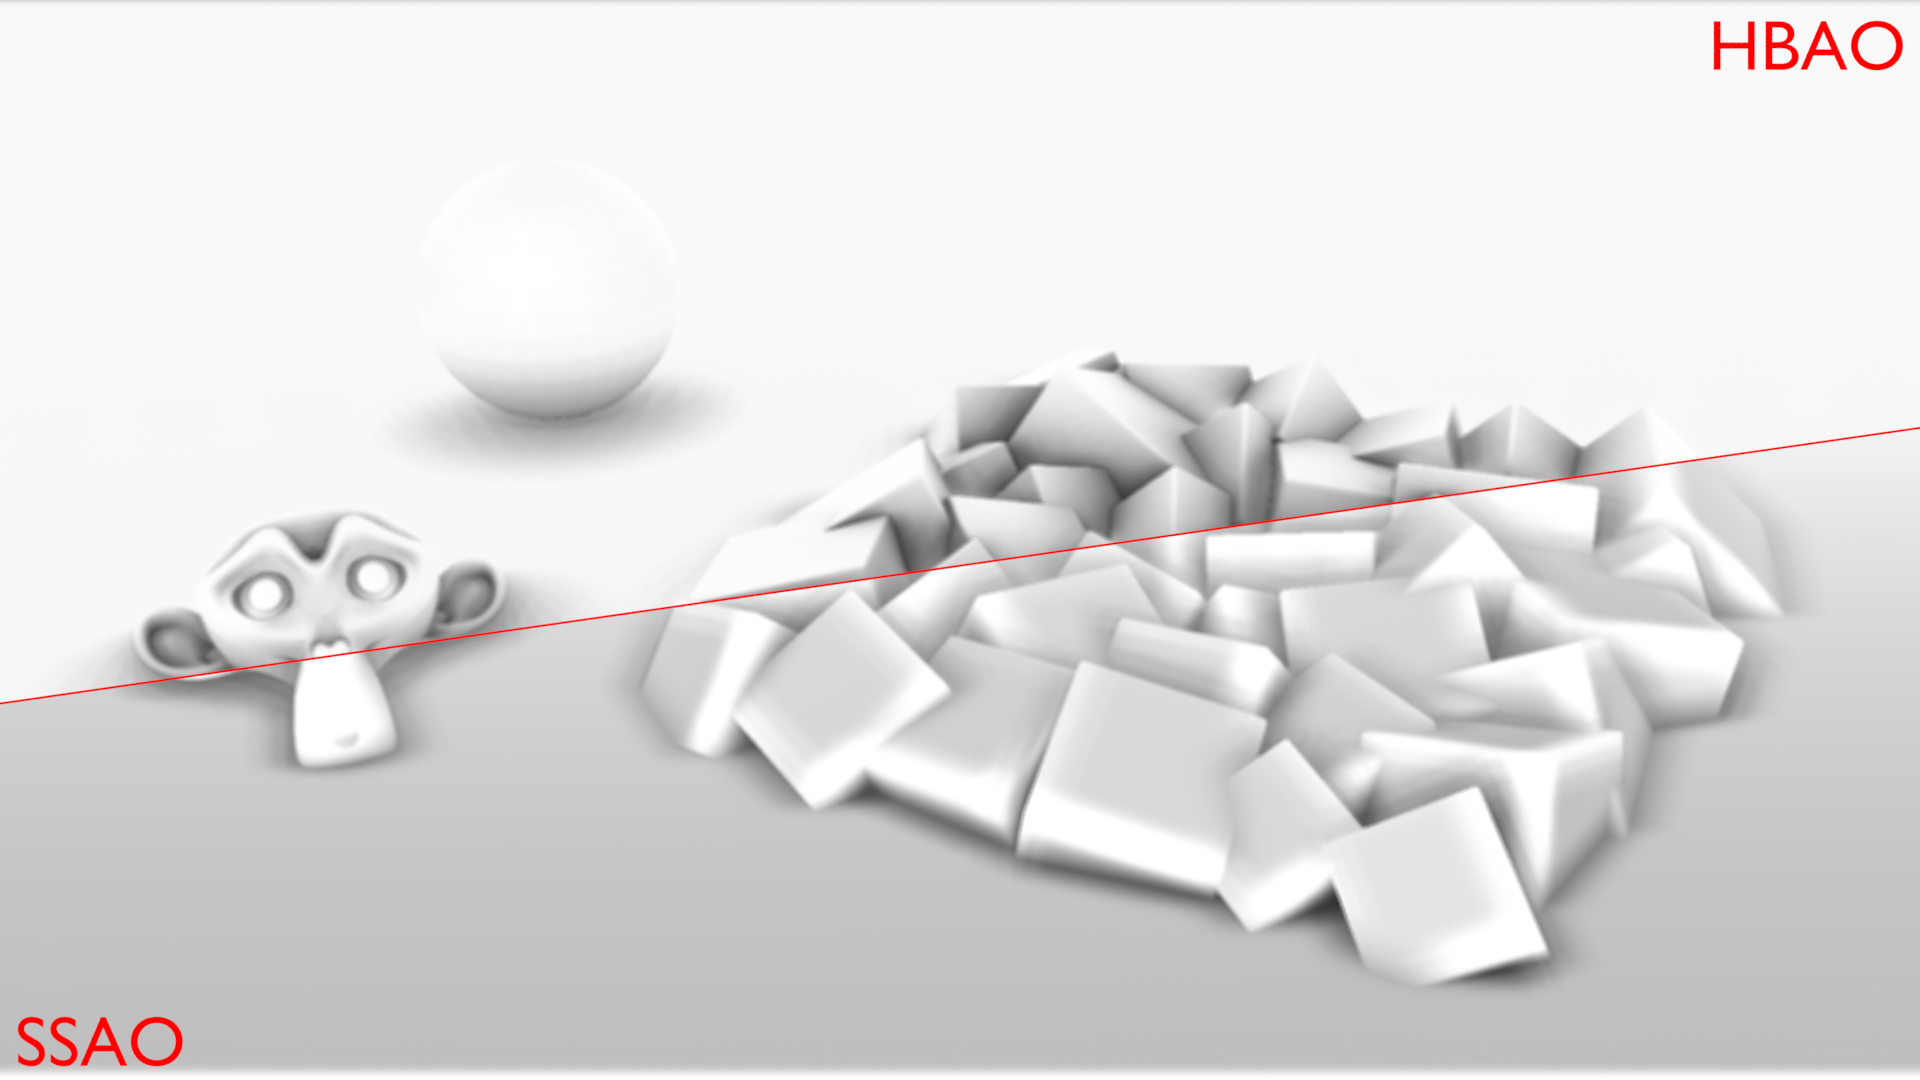
\includegraphics[width=24em]{images/navrh/ssao-hbao.png}
	\caption[caption]{Porovnávní SSAO a HBAO. Metoda HBAO nabízí reálnější zobrazení více připomínající reálný svět. Obrázek zobrazuje pouze ambient oclusion.\footnotemark} 
	\label{ssao-hbao-comp}
\end{figure}

\footnotetext{Obrázek převzat z: \href{https://blenderartists.org/t/bge-hbao-ambient-occlusion-shader/690374}{https://blenderartists.org/t/bge-hbao-ambient-occlusion-shader/690374}}

Jak bylo zmíněno v~sekci \ref{ssao-theory}, musí se výsledek SSAO funkce rozmazat, jinak je viditelný šum. To bude v~práci vyřešeno zprůměrováním okolních hodnot. Tím se docílí sice mírně rozmazaného obrazu, a může se stát, že bude okluze v~některých místech silnější nebo slabší než by měla být, ale efekt je to stále dostatečný.


\section{Návrh knihovny}
Knihovna bude vytvořena tak, že jejím vstupem bude konfigurace a koordináty oblasti, která se bude generovat. Uživatelsky dostupné budou hlavně funkce na nastavení vlastní konfigurace, zapnutí generace (která poběží asynchroně) a zrušení generování, pokud ještě nedoběhlo. Knihovna bude zpočátku vracet vše v~nízkém rolišení, které bude s~postupem času zvyšováno. To urychlí generování alespoň základního modelu. Zároveň bude s~postupem času model stále více kvalitní a reprezentace světa bude přesnější. Generování vegetace proběhne právě jednou, a to až bude generovaná mapa o~dostatečně vysokém rozlišení, aby bylo zobrazení relativně přesné.

Ke knihovně budou také dostupné soubory s~texturami pro generovanou oblast a veškerými modely vegetace. Modely se kterými bude knihovna pracovat budou ve formátu OBJ\footnote{\href{https://en.wikipedia.org/wiki/Wavefront_.obj_file}{Wavefront OBJ (Wikipedia)}}, který je jednoduše zpracovatelný a dostatečný pro tuto práci. Knihovna bude obsahovat logovací funkce, do které si uživatel knihovny bude moct vložit vlastní funkci jako výstup logu a bude moct takto postupně získávat informace o~tom, co knihovna zrovna generuje. Po volání funkce na generování knihovna vrátí prázdný objekt reprezentující mapu, která bude postupně zaplněna daty podle toho co bude zrovna vygenerováno.

\subsection*{Výstup knihovny}
Výstupem bude scéna obsahující veškeré modely, jejich textury, shadery, programy (sbírka zkompilovaných shaderů pro grafické karty) a další popis, jak scénu správně zobrazit (uniformní proměnné atd.). Každý model může využívat více programů, každý program musí obsahovat minimálně vertex a fragment shader, ale může nepovinně obsahovat i geometry tessalation control, a tesslation evaluation shader. Každý takovýto shader bude moct být využit u~více různých programů. Dále bude u~programu nastavitelné, jestli se má zobrazit do nějaké konkrétní textury, nebo do libovolného bufferu, který je zrovna aktivní. Krom toho budou na program vázány textury, které budou stejně jako shadery využitelné pro více programů zároveň. Na obrázku \ref{out-dia} je dostupný diagram této scény.
\begin{figure}[H]
	\centering
	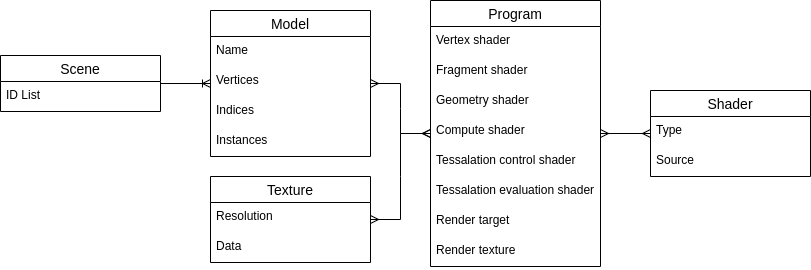
\includegraphics[width=38em]{images/navrh/scene_diagram.png}
	\caption[caption]{Diagram popisu jak vypadá scéna, která je výstupem knihovny. Zakončení čar symbolizuje vztah mezi prvky. Jednoduché značí 1:n, větvené m:n} 
	\label{out-dia}
\end{figure}

Takto vytvořená scéna nemusí nutně obsahovat pouze mapu, ale teoreticky cokoliv jiného.

\subsection*{Konfigurace knihovny}
Knihovna by měla být co nejvíce konfigurovatelná tak, aby uživatel mohl nastavit co nejvíce parametrů generování. Bude se jednat o~parametry:

\begin{itemize}
    \item maximální a minimální rozlišení textury, určující typ oblasti
    \item jak velký je krok mezi jednotlivými generovanými rozlišeními
    \item rozlišení výškové mapy oblasti
    \item minimální rozlišení potřebné k~vygenerování vegetace
    \item počáteční hodnota generátoru náhodných čísel použitého při generování vegetace
\end{itemize}

Krom toho bude muset uživatel dodat API klíč pro Bing Maps, které nedovolují přístup bez něj. Konfigurace bude předána jako JSON soubor, který se předá jako argument při spouštění aplikace, a bude obsahovat všechna tato nastavení.


\section{Návrh uživatelské aplikace}
Uživatelská aplikace bude rozdělena na dvě hlavní části. V~první z~nich bude na výběr klasická 2D mapa, na které si uživatel bude moct vybrat jakou oblast chce zobrazit, a další prvky pro ovládání a potvrzení výběru. Druhá část bude obsahovat prvky, které budou nastavovat chování zobrazovaného modelu, model samotný a tlačítko zpět, kterým se uživatel dostane zpět k~části s~výběrem oblasti.

\subsection*{Rozhraní mapy}
Mapa bude zabírat většinu prostoru okna. Kromě mapy zde bude dostupná lišta pro uživatelský vstup, do které uživatel zadá vyhledané místo, a tlačítko na potvrzení vyhledávaného dotazu. Dále bude k~dispozici potvrzení vybrané oblasti a zahájení generování oblasti. Pro zobrazení 2D mapy bude využito knihovny \verb|Marble|, která je součástí aplikace pod stejným názvem. \verb|Marble| je open-source přenositelná aplikace, přestože je součástí KDE, což je desktopové prostředí pro operační systém Linux. Výběr oblasti proběhne pomocí podržení pravého tlačítka myši a potáhnutí po části mapy. Když uživatel tlačítko pustí, zobrazí se, která oblast byla vybrána. Dále na mapě budou dostupné ovládací a informační prvky jako měřítko a přiblížení či oddálení mapy. Návrh tohoto rozhraní je dostupný na obrázku \ref{map-ui}.

\begin{figure}[H]
	\centering
	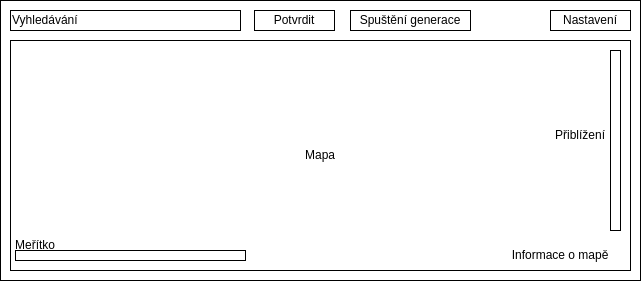
\includegraphics[width=38em]{images/navrh/map-view.png}
	\caption[caption]{Návrh uživatelského rozhraní pro vybírání oblasti ke generaci} 
	\label{map-ui}
\end{figure}

Většina ovládacích prvků mapy bude možné schovat a zobrazit po kliknutí pravým tlačítkem myši bez potáhnutí tak, aby nedošlo k~výběru oblasti.

\subsection*{Rozhraní pro generovanou oblast}
Generována oblast bude mít své vlastní rozhraní, obsahující výřez s~OpenGL kontextem (zvaná renderer) a ovládací prvky pro tento kontext. Bude zde možnost zapnout a vypnout prvky, o~které se stará renderer, a ne knihovna samotná. Součástí bude i tlačítko zpět, aby se uživatel mohl vrátit do výběru oblasti a nebyl nucen aplikaci restartovat pokaždé když chce vybrat jinou oblast. Zároveň zde bude dostupná plocha pro výstup z~logovací funkce knihovny, protože zde může uživatel čekat delší dobu, než se například stáhnou metadata pro oblast.


\begin{figure}[H]
	\centering
	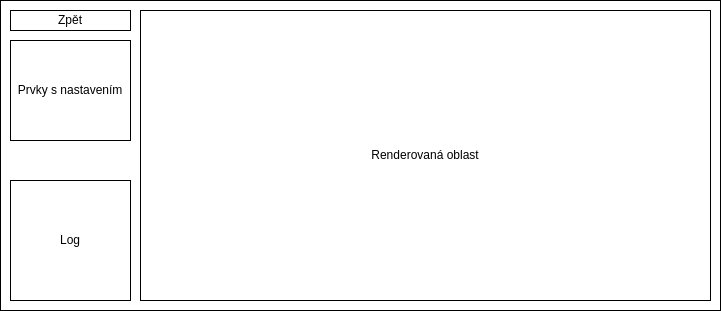
\includegraphics[width=38em]{images/navrh/renderer-ui.png}
	\caption[caption]{Návrh uživatelského rozhraní pro zobrazení generované oblasti} 
	\label{renderer-ui}
\end{figure}

Na obrázku \ref{renderer-ui} je návrh toho, jak tato oblast bude vypadat.

\subsection*{Zobrazení generované oblasti}
V~této oblasti zvané renderer se bude zobrazovat výstup z~knihovny. Vzhledem k~tomu, že výstupem jsou pouze objekty, a ne další post-process efekty jako AO, je nutné tyto efekty přidat později. Renderování výstupu bude provedeno metodou deffered shading, která dovoluje jednoduché přidávání post process efektů. Zároveň se bude starat o~další funkcionalitu typu odebírání počtu vegetace, což je vhodné pro zvýšení výkonosti aplikace (větší oblast obsahující vysoké množství vegetace může mít problémy), nebo také pro zlepšení viditelnosti například lesních cest, které mohou být jinak hůře viditelné přes vegetaci. Mimo jiné bude možné nastavit sílu tohoto odebírání tak, aby uživatel dosáhl požadovaného výsledku. Renderer bude schopný zobrazit libovolnou scénu, která obsahuje libovolný počet modelů, shaderů a dalších grafických objektů. Renderované scéně bude poskytovat informace jako uplynulý čas, časový rozdíl mezi jednotlivými snímky, pozici kamery, a další. Obnovovací frekvence bude limitována podle obrazovky na uživatelském zařízení. To zde bude z~důvodu, aby aplikace zbytečně nezatěžovala výpočetní zdroje, které nejsou nutně potřebné. Zobrazení oblasti bude nastavené tak, aby směr, kterým je sever, byl po vytvoření aplikace vždy směrem vpřed, východ vpravo atd. Toto zobrazení bude využívat metodu deferred shading pro jednodušší implementaci post-process efektů.

\chapter{Implementace aplikace}
V~této kapitole je popsána praktická část této práce. Práce je rozdělená na 3 hlavní části -- generování mapy, zobrazení výsledku a uživatelské rozhraní. Generování mapy je umístěno do svého vlastního projektu, který nemá žádnou závislost na zbytku.


\section{Generování mapy}
Generování mapy je rozděleno do několika fází. V~první z~nich jsou získány informace o~oblasti, a pak je postupně generováno detailnější zobrazení těchto dat. Generování samotné je rozděleno tak, že generování jednotlivých typů objektů (povrchy, budovy, vegetace atd.) běží postupně každé zvlášť.

\subsection*{Generování povrchu} \label{impl-gen-surface}
V~první fázi jsou stažena data z~Bing Maps API. Aplikace pošle 1 -- 9 požadavků na API dle nastavení, a poté je poskládá do mřížky, ze které jsou vypočteny trojúhelníky a jejich normálové vektory. Takto poskládaný povrch je umístěn mezi koordináty 0 -- 1 jak pro x, tak pro z. Výšková data jsou rozděleny tak, aby prostřední bod výšky byl umístěn na pozici 0.5. Jelikož data získána z~API jsou v~metrech nad mořem, musí se provést normalizace tak, aby data odpovídala rozměrům modelu, a dala se zobrazit. To je provedeno tak, že k~normalizaci, která by standartně vygenerovala nejvyšší bod na pozici 1 a nejnižší na pozici 0, jsou před počítáním minimální a maximální výšky přidána ještě data o~délce a šířce oblasti samotné. Jelikož mají známý rozměr od 0 do 1, odpovídají takto normalizované hodnoty realitě.

\begin{align}
 realHeight &= \frac{currentHeight - minHeight}{maxHeight - minHeight} \nonumber
\end{align}

Jelikož data jsou v~této fázi v~relativně nízkém rozlišení, maximálně 96x96 výškových bodů, je při jejich zobrazení provedena tessalace\footnote{Proces rozdělení jednoho polygonu na více menších.}. Implementace tessalace je v~práci provedena jako metoda PCCM, která běží jako tessalační shader na grafické kartě. Implementace byla inspirována článkem z~\cite{ogldev}.

Protože je výšková mapa interpolována až při renderování, může se stát, že změna tvaru je dostatečná na to, že některé prvky vykreslované později mohou být vytvořeny mimo povrch. To je řešeno tak, že veškerý povrch je vyrenderován dvakrát. První render proběhne z~pohledu tak, aby uživatel viděl mapu. Druhý probíhá ze shora nad povrchem, a zobrazí do textury pouze výškovou složku povrchu. Výsledná textura z~tohoto renderu je následně předána dalším objektům, které jsou renderovány na povrch, a jejich pozice je založena právě na hodnotách získaných z~této textury.

\subsection*{Získávání a generování metadat} \label{impl-metadata-gen}
Poté, co je vygenerován povrch, jsou stažena metadata z~OpenStreetMap. Jakožto OpenStreetMap samotné nejsou vhodné na čisté získávání informací o~oblasti, je v~projektu využito Overpass API\footnote{\href{https://wiki.openstreetmap.org/wiki/Overpass_API}{ttps://wiki.openstreetmap.org/wiki/Overpass\_API}}, které je optimalizované na čtení dat. Pro libovolnou oblast se pošle požadavek, který získá veškerou geometrii pro každý objekt v~oblasti. Geometrie je definována jako seznam bodů, které jsou definovány svou zeměpisnou výškou a šířkou. Dále jsou získány informace o~každém takovém objektu. Mezi tyto informace patří hlavně typ objektu a další metadata (u~lesu například typ, u~budovy počet pater apod.). API tyto informace vrací ve formátu JSON, a pro konverzi do C++ objektu je využito knihovny \verb|JSON for Modern C++|\footnote{\href{https://github.com/nlohmann/json}{https://github.com/nlohmann/json}}. 

Tyto informace jsou následně zpracovány do textury, která dle barvy každého pixelu určuje typ oblasti, která je zde obsažena. Textura obsahuje 4 hodnoty typu float, a je tedy teoreticky omezena na 2\textsuperscript{128} oblastí, což je podstatně více než API poskytuje. Jednotlivých typů oblastí, které aplikace rozpoznává, je 42, a jsou navíc rozděleny do 12 kategorií. Jedná se o~lesy, louky, zahrady, vodní plochy, farmy, cesty (asfaltované, chodníky, lesní cesty), písčité oblasti a okraje měst. Lesy jsou dále rozděleny za listnaté, jehličnaté a smíšené. Podle toho se v~aplikaci chová generování vegetace.
\begin{figure}[H]
	\centering
	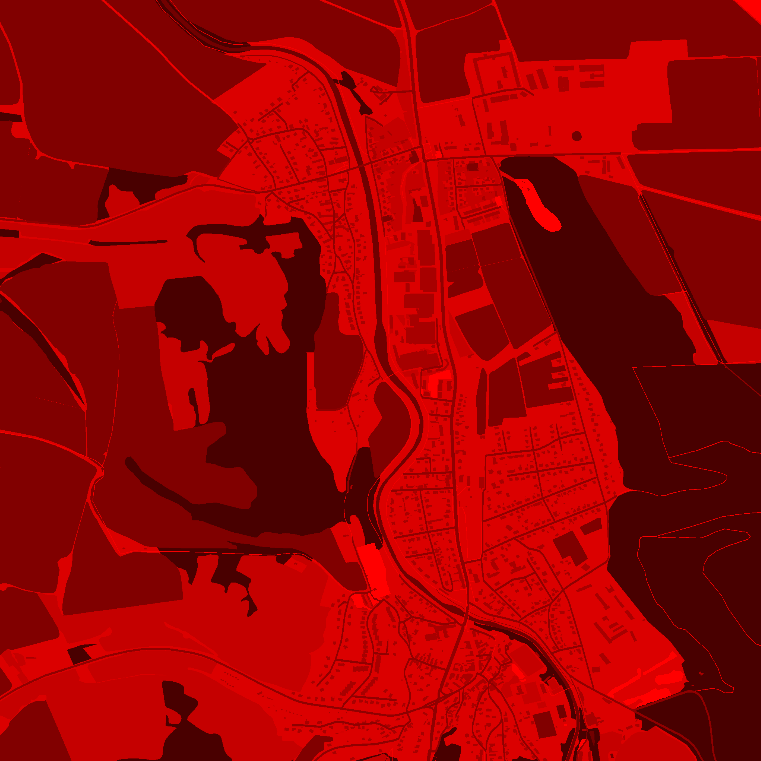
\includegraphics[width=20em]{images/impl/metadata.png}
	\caption[caption]{Ukázka vygenerovaných metadat o~typu oblasti. Obrázek je zesvětlen pro lepší viditelnost.} 
	\label{metadata-img}
\end{figure}

Na obrázku \ref{metadata-img} je vidět ukázka metadat o~takto vygenerované oblasti. Všechny informace jsou zde uloženy pouze v~červeném kanále, který je dostatečný na uložení všech typů oblastí, které práce rozpoznává.

Textura je vytvořena tak, že pro každý pixel je získána oblast, a její ID je uloženo do textury. Každý pixel této textury může obsahovat více oblastí, a je proto nutné zvolit správnou oblast. To probíhá primárně podle priority (např. cesty mají vyšší prioritu než vodní plochy, aby se nestalo, že řeka je nad mostem), a pokud má více oblastí stejnou prioritu, vybere se ta, která zabírá nejmenší plochu. Takto je vybrán nejvhodnější typ oblasti pro každý pixel. Na mapě obsahující velké množství oblastí (např. vysoký počet domů) tento přístup může trvat dlouhou dobu, a v~aplikaci je proto výpočet rozdělen na počet dostupných procesorových jader kromě dvou, které zůstávají volné na další výpočty.

\begin{figure}[H]
	\centering
	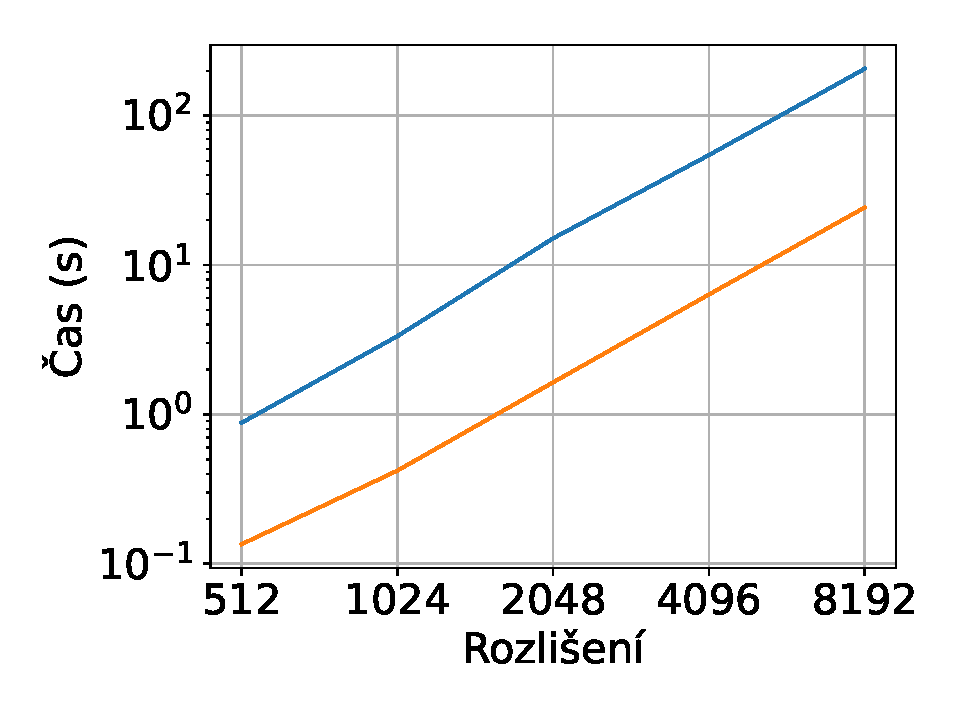
\includegraphics[width=18em]{images/impl/graphs/metadata_log.pdf}
	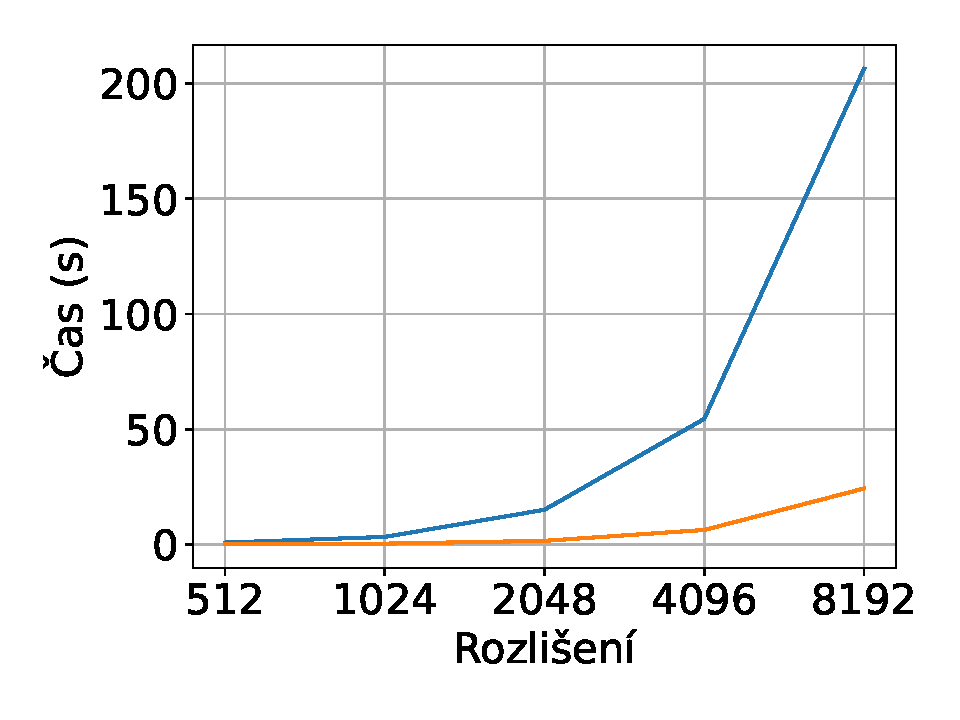
\includegraphics[width=18em]{images/impl/graphs/metadata_linear.pdf}

	\caption[caption]{Ukázka zrychlení na 16 vláknovém procesoru AMD Ryzen 7 2700. Modré části grafů znázorňují jedno vlákno, oranžové všechny. Vlevo je graf s~logaritmickým měřítkem, vpravo s~lineárním.} 
	\label{metadata-graph}
\end{figure}
Na paralelizaci výpočtu byla použita knihovna \verb|OpenMP|\footnote{\href{https://www.openmp.org/}{https://www.openmp.org/}}. Díky ní bylo dosáhnuto téměř lineárního škálování, které je zobrazené na obrázku \ref{metadata-graph}.

Před generováním mapy je třeba data získaná z~API připravit na výpočet. Příprava probíhá tak, že každé oblasti je přiřazeno její ID. Oblasti, které aplikace neumí rozpoznat, jsou zahozeny, a oblasti rozdělené na několik polygonů jsou pospojovány do jednoho velkého, což zjednodušuje výpočet. Takto vytvořená textura je pak přiřazena vygenerované ploše, která při následném vykreslování přiřazuje textury a barvy podle ID oblasti v~textuře. Tyto textury byly získány z~\href{https://www.textures.com/}{https://www.textures.com/} a \href{https://polyhaven.com/}{https://polyhaven.com/} Pokud existuje takový pixel, který nemá známou oblast, je mu přiřazena šedá barva, která působí neutrálně.


\subsection*{Generování budov}
Generování budov probíhá tak, že se ze stávajících metadat upravených ve fázi \ref{impl-metadata-gen} vyfiltrují pouze budovy, a na nich se provádí výpočet. Pro každou budovu se nejdříve zkontroluje, jestli nějaké její rohy nejsou mimo generovanou oblast. V~případě, že by byly, dojde k~tomu, že textura s~informací o~výšce popsaná v~sekci \ref{impl-gen-surface} nebude obsahovat tyto rohy, a budova nebude mít informaci o~tom, jak má být vysoko. Rohy budovy jsou posunuty tak, aby se blížily k~okraji generované plochy. Aby byl zachován co nejpřesnější tvar budovy, je zde vypočítána rovnice přímky mezi posledním bodem, který je stále uvnitř, a prvním bodem mimo. Nový bod je pak umístěn na tuto přímku co nejblíže okraji plochy. Pokud je mimo generovanou oblast více bodů, jsou odebrány všechny, a místo nich jsou vytvořeny pouze dva nové body na hranici plochy. Po této úpravě tvaru budovy je kombinace původních a nově vytvořených bodů zaslána jako vstup knihovně \verb|CDT|\footnote{\href{https://github.com/artem-ogre/CDT}{https://github.com/artem-ogre/CDT}}, která provede triangulaci, a výsledné trojúhelníky jsou použity na sestrojení podlahy a stropu budovy. Stěny jsou vytvořeny postupným propojením bodů střechy a stropu. Všechny budovy jsou postupně vkládány do jednoho modelu. I~velmi vysoký počet budov na mapě má nízký vliv na výkon, a není potřeba je tedy odebírat, aby se snížil potřebný výkon. Celé město Brno obsahuje 4,5 milionu trojúhelníků v~budovách, což moderní grafické karty zvládají bez problémů. Protože budovy není potřeba odebírat, jsou všechny poskládány do jednoho modelu pro jednoduchost zobrazování, nastavování textur a podobných vlastností.

\begin{figure}[H]
	\centering
	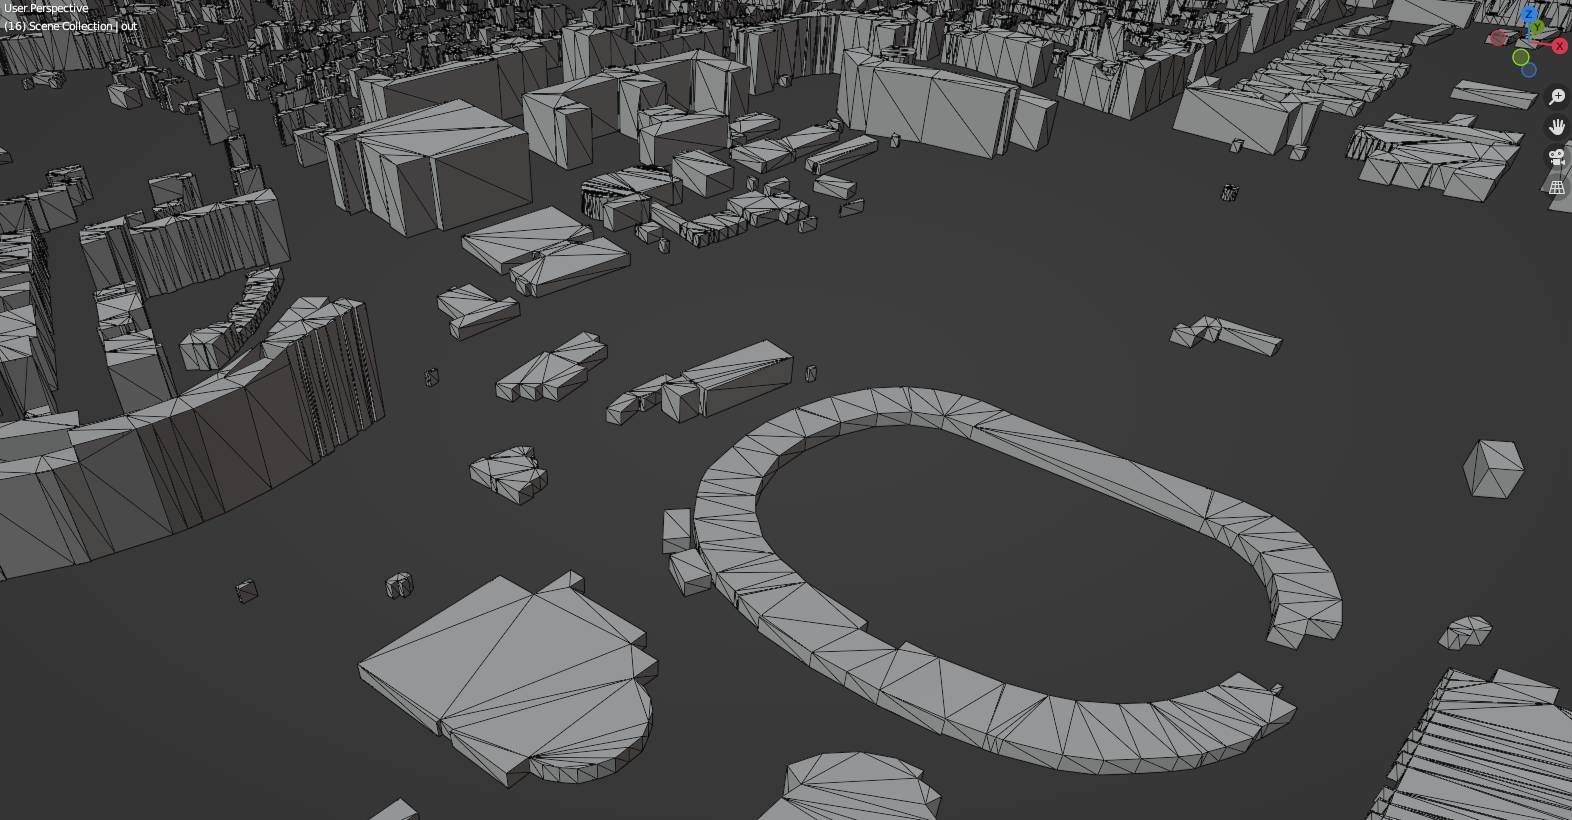
\includegraphics[width=32em]{images/impl/buildings.png}
	\caption[caption]{Ukázka vygenerovaných budov po exportu z~aplikace a importu do aplikace Blender. Na obrázku je možné vidět wireframe budov.} 
	\label{buildings-gen}
\end{figure}

Generování budov proběhne hned po vygenerování základní mapy s~nejnižším rozlišením. Triangulace i pro velké oblasti jako je město Brno proběhne pro všechny budovy pod sekundu a není tedy nutné ji nijak zvlášť paralelizovat. Na obrázku \ref{buildings-gen} je ukázka generovaných budov.

\subsection*{Generování vegetace}
Generování vegetace proběhne až poté, co je rozlišení textury určující typ oblasti v~dostatečně vysokém rozlišení. Výchozím nastavením je, že generování proběhne, až když je rozlišení textury alespoň 1024 pixelů. To je v~aplikaci z~toho důvodu, aby generování vegetace bylo co nejpřesnější, protože na rozmístění oblasti využívá právě tuto texturu. 

Generování samotné pak probíhá tak, že prvně jsou při vytvoření třídy načteny všechny modely, které budou při generování použity. Na jednotlivý typ vegetrace je možné použít několik různých modelů uložených do \verb|.obj|\footnote{\href{https://en.wikipedia.org/wiki/Wavefront_.obj_file}{https://en.wikipedia.org/wiki/Wavefront\_.obj\_file}} souborů. Ty stačí vložit do správné podsložky ve složce \verb|lib/assets/models| a program je automaticky načte a náhodně promíchá s~ostatními stejného typu. Po vytvoření generátoru je možné začít generovat vegetaci. Na každý typ vegetace je nutné zavolat funkci, která generuje vegetaci s~jiným nastavením, a to proto, že například stromy mají jinou hustotu umístění a výšku oproti například obilí. Podporované typy vegetace jsou jehličnaté, listnaté a smíšené lesy a pole. Generování probíhá tak, že je vypočtena hustota a výška vegetace, a poté jsou zavolány funkce z~knihovny \verb|poisson-disk-sampling|\footnote{\href{https://github.com/thinks/poisson-disk-sampling}{https://github.com/thinks/poisson-disk-sampling}}. Z~této knihovny je možné získat seznam bodů, které značí umístění jednotlivých vygenerovaných pozic. Pro každý takový bod je zkontrolováno, jestli je umístěn uvnitř nebo mimo oblast, pro kterou se generuje vegetace. Tato kontrola se provádí oproti textuře s~metadaty. Body, které jsou mimo, jsou zahozeny. Poté je pro každý bod určený náhodný druh vegetace -- například v~případě smíšeného lesa je určeno, zda se jedná o~listnatý nebo jehličnatý strom, a k~modelu stromu je přidána informace o~pozici bodu. Tato pozice je generována od 0 do 1 a s~její hodnotou se počítá jako s~offsetem vegetace oproti její výchozí pozici.

\begin{figure}[H]
	\centering
	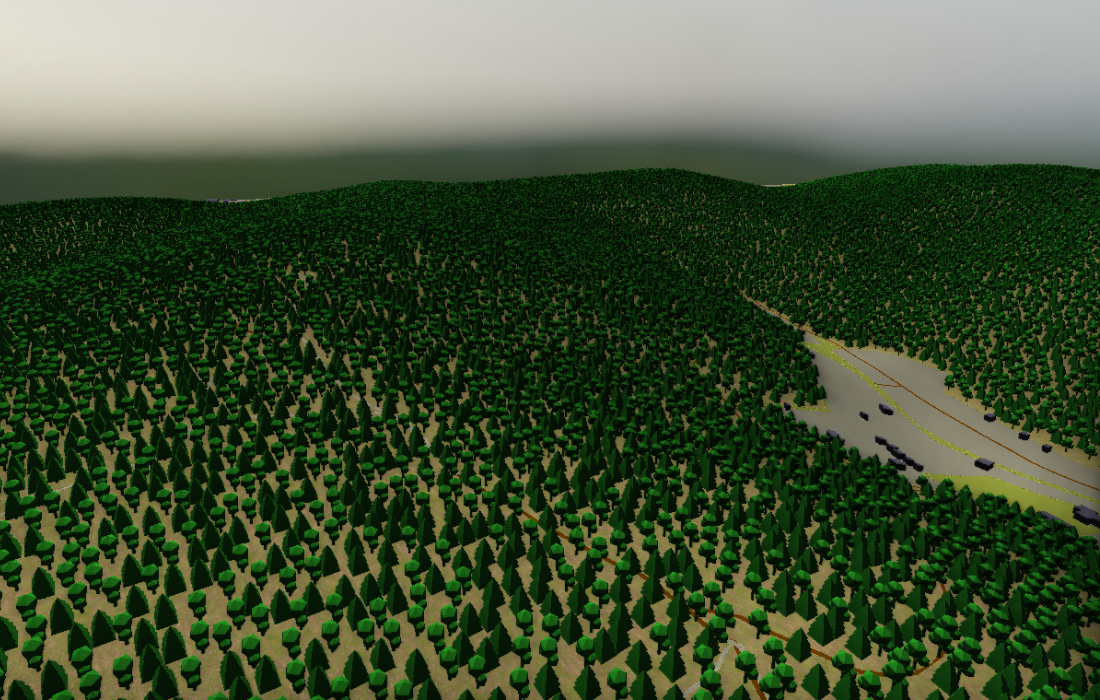
\includegraphics[width=18em]{images/impl/trees.png}
	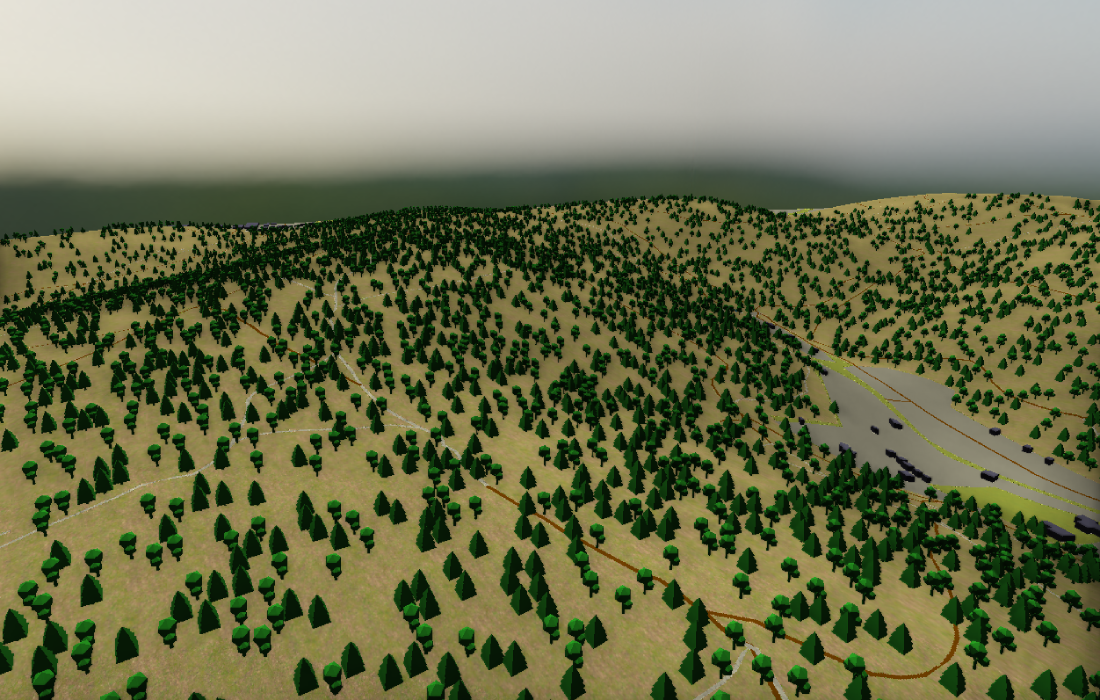
\includegraphics[width=18em]{images/impl/trees_culled.png}
	\caption[caption]{Ukázka vygenerovaného smíšeného lesa. Vlevo jsou vidět všechny stromy, vpravo je les po odebrání vegetace, nastaveném na maximální hodnotu.} 
	\label{veg-gen}
\end{figure}


Modely jsou vytvořeny tak, aby obsahovaly co nejméně trojúhelníků (celý jehličnatý strom má pouze 90), ale to samotné není dostatečné na to, aby byl výkon přijatelný. V~případě větších oblastí může vygenerovaná vegetace zabírat velké množství výkonu, a z~toho důvodu je při zobrazování odebírána vzdálená vegetace. Pro celé město Brno je generováno téměř půl milionu jednotlivých kusů vegetace. Po přepočtu na polygony je to přibližně 1,5 miliardy trojúhelníků. Ani moderní grafický hardware na toto nemá dostatečný výkon -- okolo 10 snímků za sekundu na grafické kartě \verb|Nvidia GTX 1080|. Odebereme-li přebytečnou vegetaci, počet snímků za sekundu se zvýší na přibližně 50 pro stejnou scénu.

Další výhodou toho, že jsou stromy odebírány, je to, že po odebrání je možné vidět nové lesní cesty, které jinak nemusí být viditelné. Ukázka vygenerované vegetace je na obrázku \ref{veg-gen}.

\subsection*{Skládání výsledků}
Každý z~vygenerovaných objektů je vrácen do třídy, která se stará o~skládání jednotlivých objektů. Ta objekty vygeneruje a vloží do scény (mapy). Tato třída se zároveň stará o~veškeré načítání všech složení programů, nastavení, které textury patří ke kterým modelům, shaderů (které jsou při kompilaci zabaleny do binárního souboru samotného), atd. Zároveň se stará o~správné předávání dat mezi jednotlivými generátory, a výslednou scénu aktualizuje pokaždé, když je to potřeba.

\section{Zobrazení výsledku} \label{render-out}
O~zobrazování výsledků se starají dvě hlavní, a několik pomocných tříd. Hlavní třídy jsou \verb|Renderer| a \verb|Scene3D|. Mezi pomocné třídy patří implementace SSAO, skyboxu a kamery, které jsou umístěny do tříd se stejným názvem jako je jejich funkčnost.

\subsection*{Renderer}
Třída \verb|renderer| se stará o~zobrazování scény a ovládání pomocných tříd jako \verb|SSAO|, které přidávají do scény další efekty. Dědí ze třídy \verb|QOpenGLWidget|, která je součásti knihovny Qt a obsahuje většinu věcí potřebných k~práci s~OpenGL. Obsahuje zejména funkce pro implementaci virtuálních metod, a funkci, která se stará o~incializaci OpenGL kontextu, kamery, post-process efektů a veškerých součásti G-bufferu, který je potřeba pro správné zobrazení scény. Když je vše správně inicializováno, je možné aby obsah mohl být zobrazován. Funkce na zobrazení scény se volá periodicky pokaždé, když je třeba nového zobrazení snímku. V~každém takovém volání proběhne nastavení správných bufferů (Qt si vytváří vlastní), vyčištění obrazovky, a následně vykreslení obrazu. Vykreslení probíhá v~několika fázích:
\begin{enumerate}
    \item Geometry pass  -- vykreslí veškerou geometrii, její normály, složku s~lesklostí a barvu do textur obsažených v~G-bufferu. Výsledek průchodu je zobrazen na obrázku \ref{geometry-pass}.
    \item SSAO pass -- vykreslí podle geometrie vrstvu ambient oclusion do vlastní textury. Renderuje se zde pouze jeden obdélník přes celou obrazovku.
    \item Blur pass -- rozostří původní výsledek SSAO tak, aby nebyl vidět šum. Výsledek tohoto a předchozího průchodu je na obrázku \ref{ssao-pass}.
    \item Lightning pass -- vypočte se veškeré nasvícení scény z~informací získaných v~předešlých průchodech, a jako výstup použije výsledný buffer.
    \item Skybox pass -- na pixely, na kterých nebylo nic umístěno v~předešlých průchodech, je umístěna obloha. Výsledná scéna po a před tímto průchodem je na obrázku \ref{lightning-pass}
\end{enumerate}

\begin{figure}[H]
	\centering
	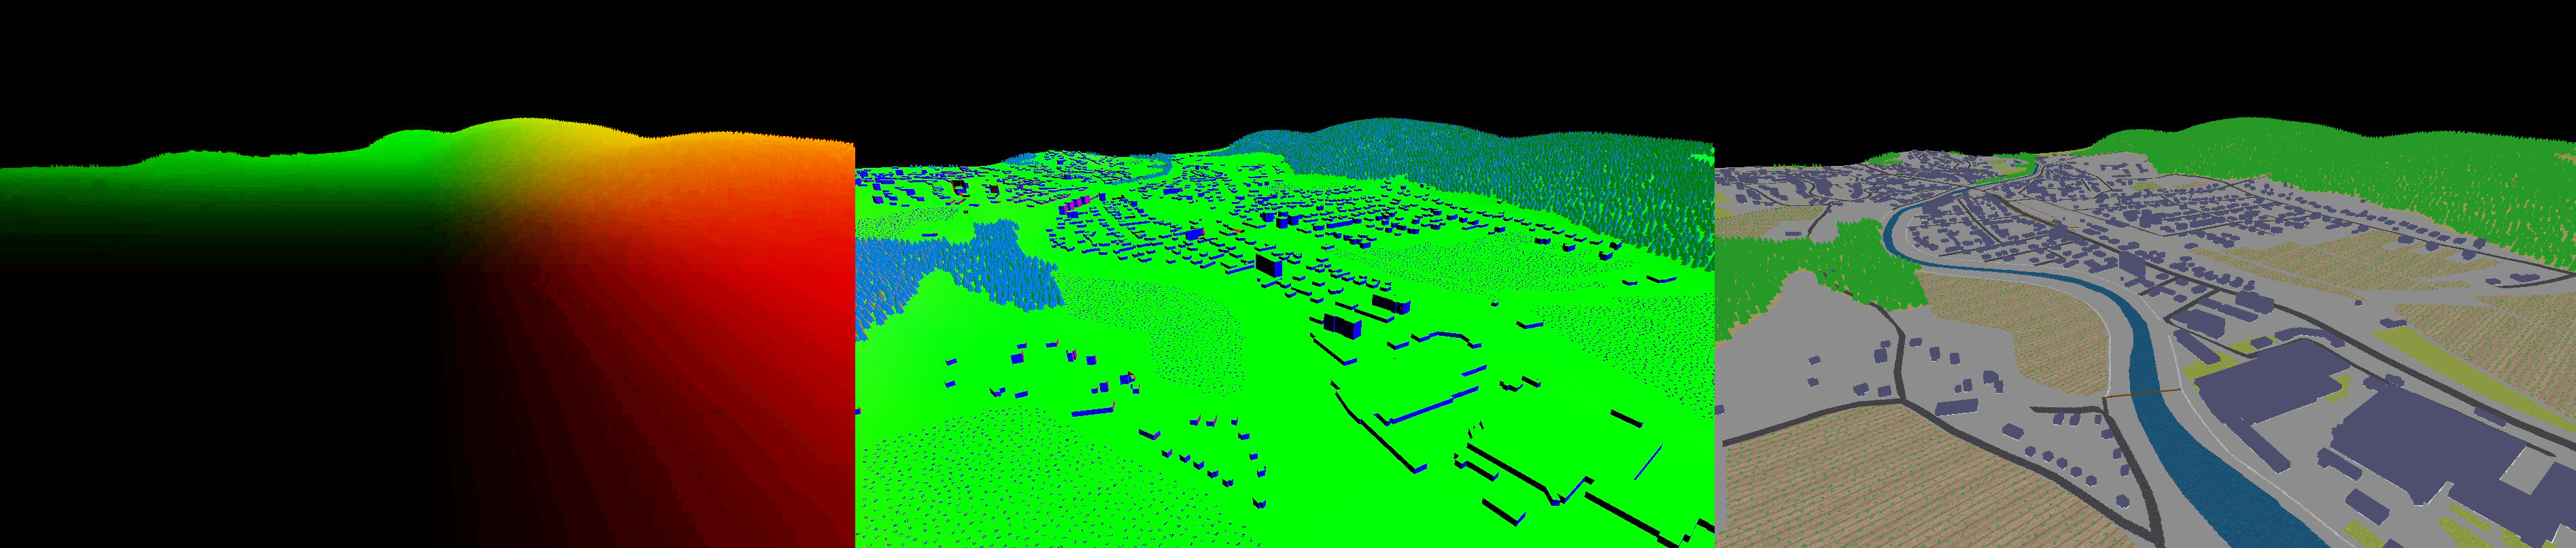
\includegraphics[width=38em]{images/impl/gbuffer/geom.jpg}
	\caption[caption]{Výstup průchodu, který vypočte geometrii. Vlevo je pozice jednotlivých pixelů, ale zesvětlena pro lepší viditelnost. Uprostřed jsou normálové vektory, vpravo je barevný výstup. Alpha složka barevného výstupu obsahuje informaci o~lesklosti.} 
	\label{geometry-pass}
\end{figure}


\begin{figure}[H]
	\centering
	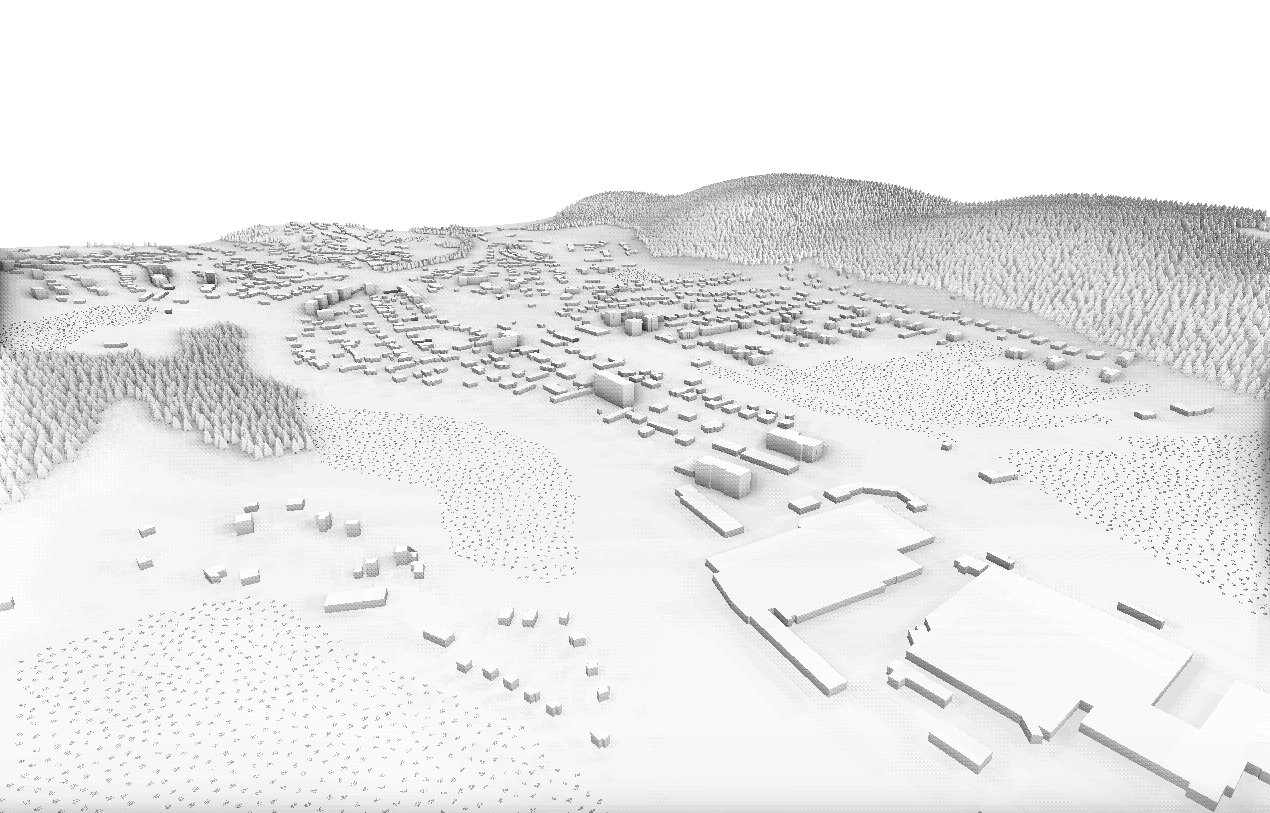
\includegraphics[width=16em]{images/impl/gbuffer/ssao.png}
	\caption[caption]{Výstup SSAO průchodu scénou. Zde je zobrazena verze bez rozmazání.} 
	\label{ssao-pass}
\end{figure}


\begin{figure}[H]
	\centering
	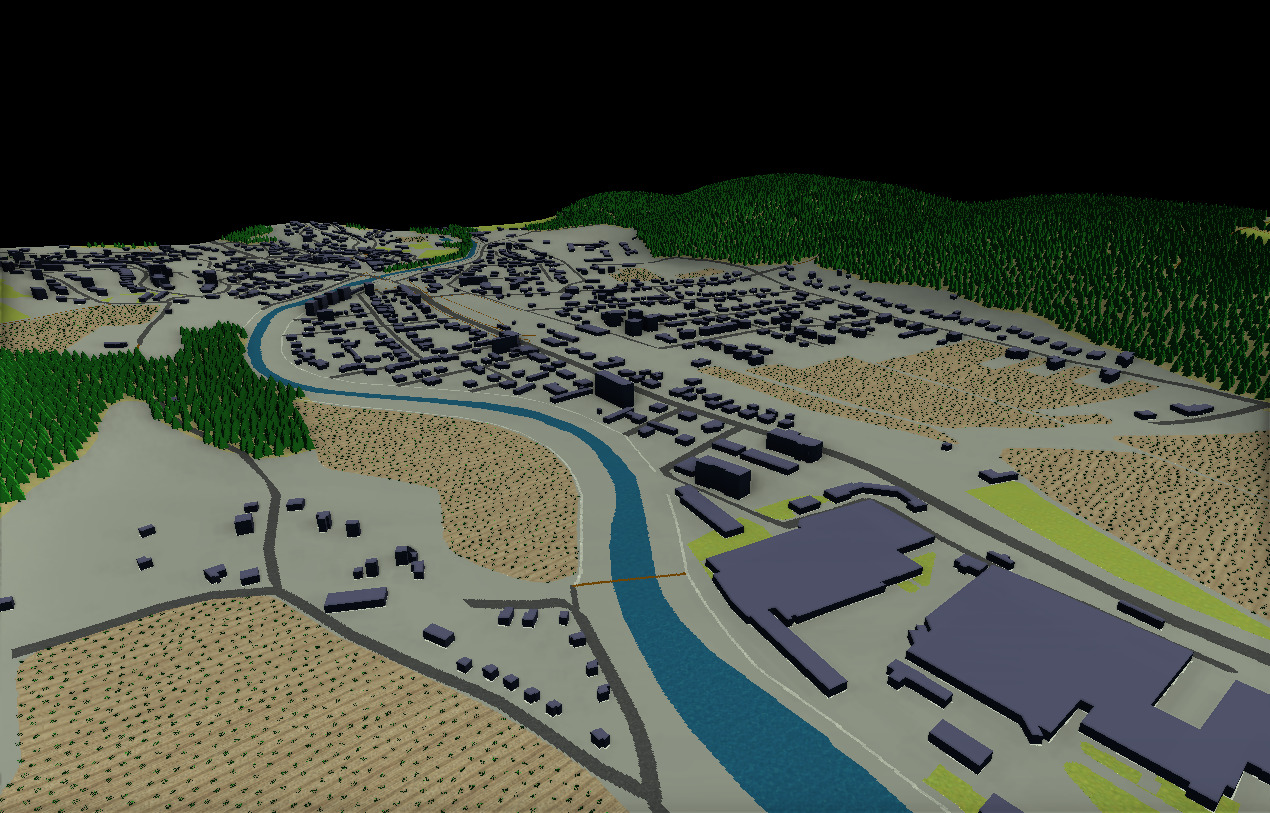
\includegraphics[width=16em]{images/impl/gbuffer/lightning.jpg}
		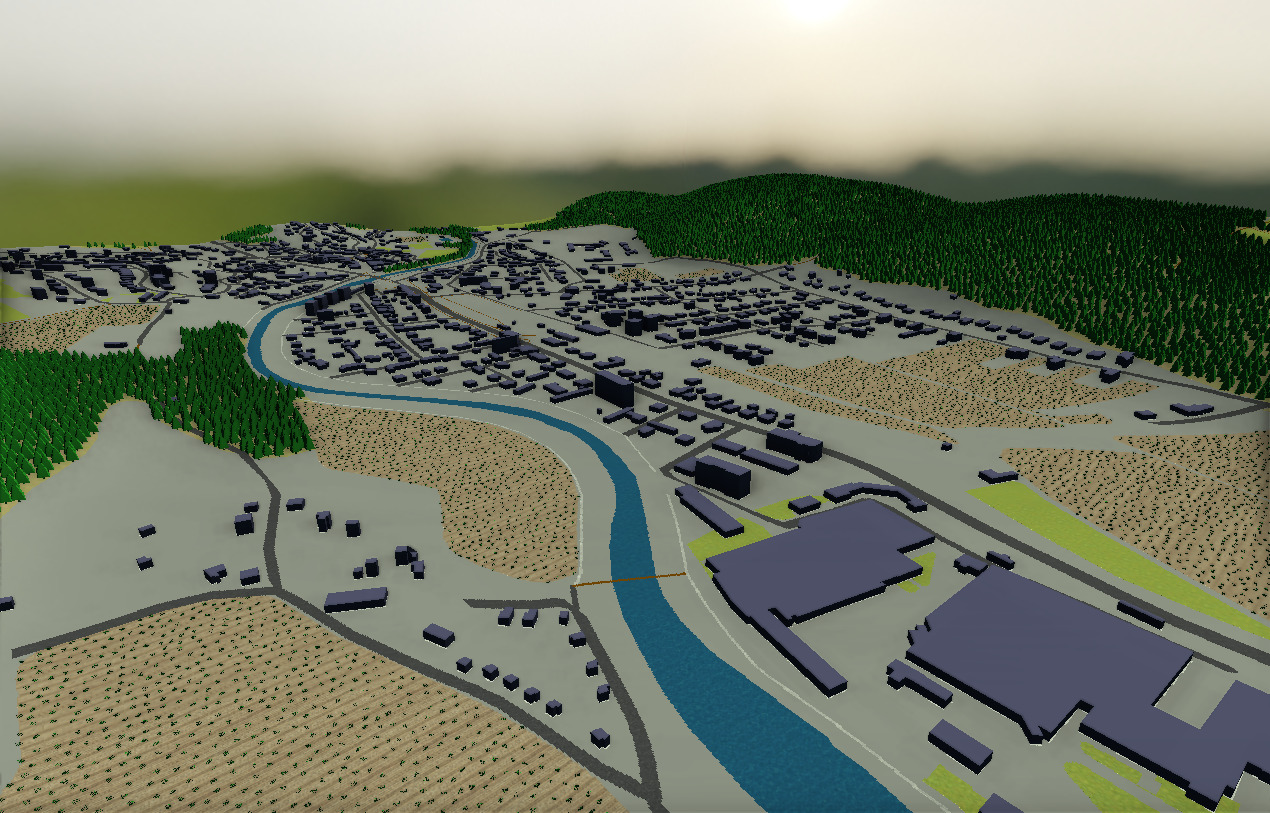
\includegraphics[width=16em]{images/impl/gbuffer/sky.jpg}
	\caption[caption]{Spočítané nasvícení scény. Vlevo je scéna po zkombinování textur z~obrázků \ref{ssao-pass} a \ref{geometry-pass}. Vpravo byla na chybějící místa do scény přidána obloha.} 
	\label{lightning-pass}
\end{figure}

Také je zde funkce, která se stará o~vytvoření nových textur, do kterých se zobrazují výsledky pokaždé, když dojde ke změně velikosti okna. To je důležité z~toho důvodu, že některé z~fází zobrazování ukládají svůj výsledek do textur, jejichž rozlišení je závislé na velikosti okna. Je tedy nutné, aby měly správnou velikost.

Dále tato třída dává vstup kameře. Vstupem pro kameru je pouze informace, že je myš na určité pozici, nebo zda je zmáčknuté tlačítko na klávesnici a na myši. Kamera pak 60x za sekundu vyhodnotí tyto vlastnosti, a podle nich vypočte novou pozici.

\subsection*{Scene}
O~zobrazení veškeré geometrie na správné pozice se stará třída \verb|Scene3D|. Jejím vstupem je přímý výstup mapy z~knihovny. Jelikož propojení jednotlivých objektů ve scéně je vyřešeno pomocí toho, že každému z~nich je přiřazeno nějaké unikátní ID, je jednoduše určeno, jestli se scéna od posledního průchodu geometrie nezměnila. Pokud je propojení jednotlivých ID na sebe jiné (např. model 8 již není propojen na texturu 6, ale 7), scény vytvoří nové objekty tak, aby bylo zobrazení vždy správné. \verb|Scene3D| se stará zároveň o~zobrazení do různých cílů (např. přímo do textury), nebo o~odebírání vzdálených kusů vegetace. Odebírání vzdálených objektů není aplikováno jen na vegetaci, ale na cokoliv, co se vykresluje pomocí metody \verb|instanced rendering|. Odebírání funguje tak, že každému objektu je přiřazena náhodná hodnota mezi 0 a 1, a následně je tato hodnota porovnána oproti vzdálenosti kamery. Pokud je vzdálenost nad toto náhodně vygenerované číslo, objekt je odebrán. Tím je docíleno postupného odebírání vegetace, které je úměrné vzdálenosti od kamery. K~náhodné hodnotě je buď přičtena nebo odečtena hodnota, kterou je určena síla odebírání. Nevýhoda tohoto přístupu je ta, že se s~každým dalším zobrazeným snímkem musí přepočítat vzdálenost kamery od všech jednotlivých instancí. To v~praxi trvalo až 6 milisekund, což významně snížilo počet snímků za sekundu, které bylo možné zobrazit. Pro docílení lepšího výkonu je tato činnost rozdělena mezi všechna jádra procesoru, čímž je potřebný čas snížen pod 1 ms na moderním hardwaru\footnote{AMD Ryzen 4500U, 15W}.

\subsection*{Implementace SSAO}
Efekt SSAO je v~práci implementován do vlastní třídy \verb|SSAO|. Ta inicializuje všechny potřebné textury a buffery pro generování tohoto efektu. Jako šum je použita náhodná textura s~rozlišením 4x4 pixely s~tím, že každý z~nich obsahuje náhodnou barvu. Jako vstup s~informacemi o~scéně jsou použity textury, které jsou výstupem metody \verb|deferred shading|. Třída na práci s~efektem si pak sama zpracuje všechny buffery tak, aby nedocházelo ke konfliktům při zobrazení dalších efektů. Jako rozmázaní výsledného obrazu, který obsahuje vysoké množství šumu, je použita funkce, která zprůměruje okolní pixely ve scéně. Tím je efekt sice mírně rozmazaný, ale stále dostatečný. Výsledek efektu je zobrazen na obrázku \ref{ssao-pass}. Implementace byla vytvořena dle \cite{learnogl} a \cite{ogldev}. Pro použití výsledné textury efektu třída obsahuje také metodu, která přiřadí výsledek na uživateli zadanou texturovací jednotku.

\subsection*{Implementace skyboxu}
Implementace skyboxu je vytvořena jako poslední fáze zobrazování scény a je ve třídě \verb|Skybox|. Ta je podobně jako SSAO nezávislá na okolí, a všechny své textury a buffery nastavuje sama. Funkčnost je taková, že se kolem kamery vytvoří dostatečně velká a vzdálená kostka s~tím, že kamera se udržuje uprostřed tak, aby uživatel nikdy nemohl vyletět mimo tuto kostku. Dostatečná velikost kostky je důležitá proto, aby se nemohlo stát, že uživatel vidí pouze část zobrazované mapy, protože zbytek je již mimo kostku. Pro sestavení výsledné skybox textury bylo využito 6 textur, které jsou poskládány na sebe, a každá z~nich je využita na jednu stěnu kostky. v~OpenGL tvoří pouze jednu texturu, jejíž typ je nastaven jako \verb|GL_TEXTURE_CUBE_MAP|. OpenGL samotné se stará o~mapování jednotlivých stěn kostky na jednotlivé textury. Jak vypadá scéna pouze se spočítaným nasvícením a po přidání skyboxu je vidět na obrázku \ref{lightning-pass}.

\section{Uživatelské rozhraní}
Uživatelské rozhraní je napsáno s~využitím knihovny \verb|Qt5|. Nepoužívá jazyk QML, ale \verb|Qt Widgets|. Celé UI je rozděleno na 3 hlavní části. První částí je hlavní okno, které pouze obsahuje další objekty, a nemá v~sobě žádnou významnou logiku (kromě nastavení, které další prvky se mají zobrazovat). Dále jsou v~aplikaci prvky pro zobrazení 2D mapy a generované 3D mapy.

\subsection*{Rozhraní na zobrazení 2D mapy}
Rozhraní funguje tak, aby bylo co nejvíce uživatelsky přívětivé. Stisknutím pravého tlačítka myši a jejím potažením si uživatel může vybrat libovolnou oblast na mapě k~zobrazení. Pokud oblast přesahuje velikost 100km\textsuperscript{2}, je uživateli zobrazeno varování, že generování a stahování oblasti může trvat dlouhou dobu. Dále je zde dostupná lišta na zadávaní vyhledávané oblasti. Vyhledávaný dotaz se dá potvrdit buď pomocí zmáčknutí tlačítka enter, nebo potvrzením pomocí tlačítka v~grafickém rozhraní.
\begin{figure}[H]
	\centering
	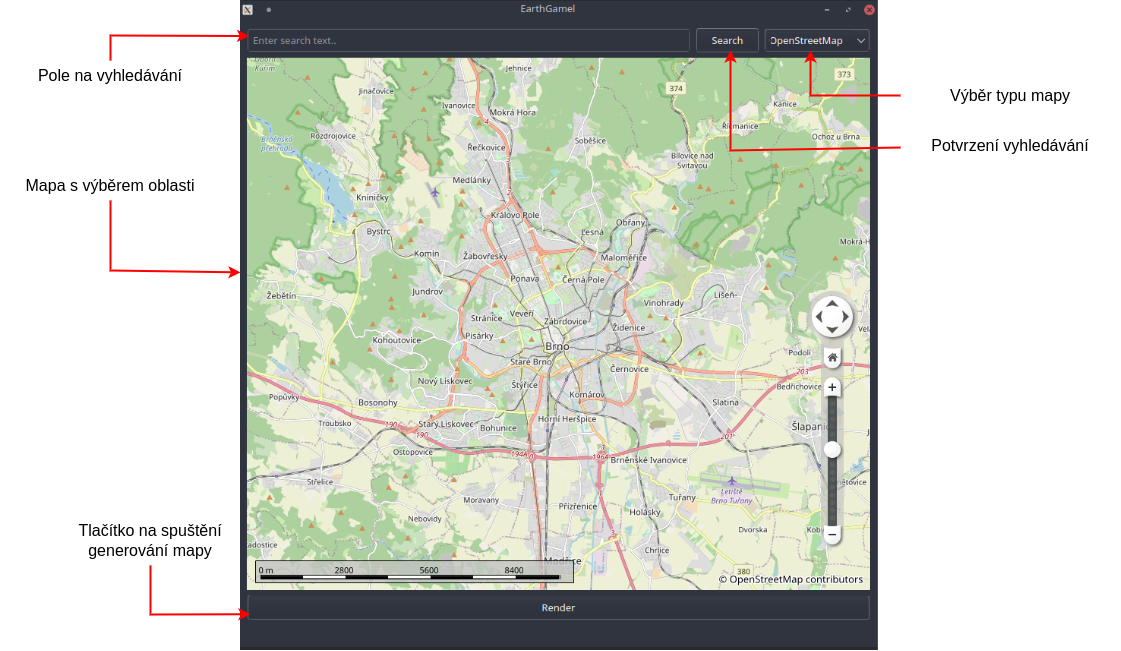
\includegraphics[width=36em]{images/impl/map-gui.png}
	\caption[caption]{Uživatelské rozhraní pro výběr oblasti na mapě.} 
	\label{gui-mapa}
\end{figure}
Dále jsou na návrhu, který je zobrazený na obrázku \ref{gui-mapa} prvky na výběr typu mapy (podporované jsou OpenStreetMap, satelitní se snímky od společnosti NASA a topografická mapa), a obsahuje i mapu samotnou. Na mapě jsou ovládací a informační prvky jako například měřítko. Ty jsou součásti knihovny \verb|Marble|, pomocí které se mapa zobrazuje.

\subsection*{Rozhraní na zobrazení výsledku}
Výsledek aplikace se zobrazuje do svého vlastního Qt Widgetu. Ten se stará o~svůj OpenGL kontext a o~vešekré ovládání a posílání událostí mezi prvky na zobrazování a Qt frameworkem. Jsou v~něm obsaženy třídy popsané v~sekci \ref{render-out}. Mezi ovládací prvky patří ovládání zobrazení (zapnutí a vypnutí jednotlivých efektů), log s~výpisem toho, co zrovna knihovna dělá, a tlačítko zpět. Ovládání je zde vytvořeno tak, že potažením po generovaném okně se posune pohled směrem, kterým uživatel potáhl. Po mapě se dá pohybovat stisknutím tlačítek \verb|W, A , S, D| na klávesnici. Alternativně se lze pohybovat i pomocí šipek. Stisknutím tlačítek \verb|Shift| a \verb|Ctrl| se nastavuje rychlost pohybu. To je vhodné použít v~případě, že je vygenerována velká oblast, ale uživatel se chce podívat pouze na malou část oblasti. Pro pohyb nahoru a dolů (přiblížení) je možné použít kolečko myši jako kdyby uživatel používal 2D mapu.

\begin{figure}[H]
	\centering
	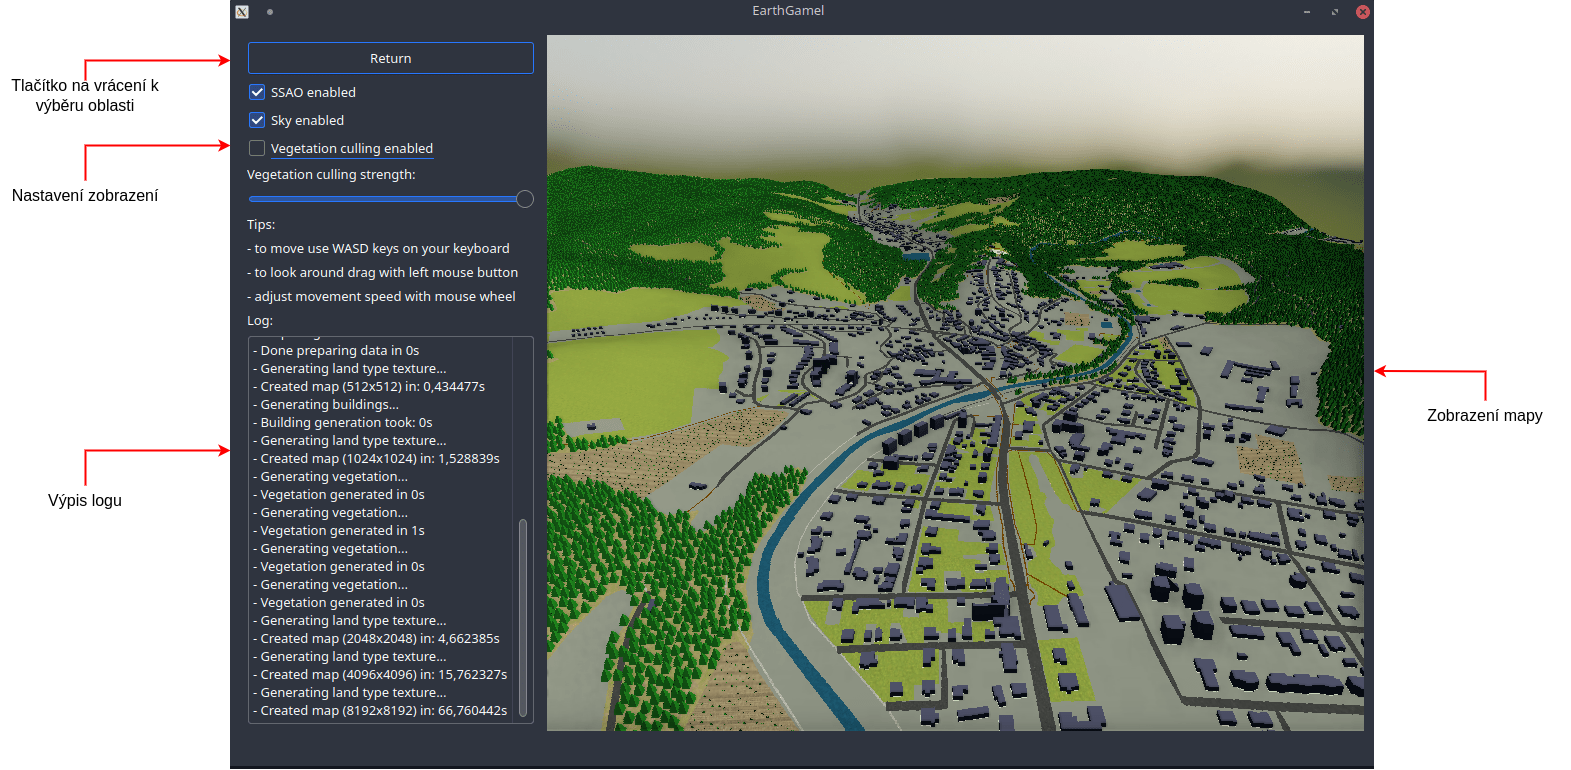
\includegraphics[width=39em]{images/impl/renderer-gui.png}
	\caption[caption]{Uživatelské rozhraní pro zobrazení generovaného výsledku.} 
	\label{gui-renderer}
\end{figure}

Popis jednotlivých prvků grafického rozhraní této části je dostupný na obrázku \ref{gui-renderer}.

Krom toho, že výstup části logu je vypisován do okna, je vypsán automaticky také do konzole, pokud uživatel spustil program z~příkazové řádky.

\section{Externí dependence aplikace}
Jak knihovna, tak uživatelské rozhraní aplikace, má několik externích dependencí. Většina z~nich je automaticky stažena a zkompilována pomocí projektu CPM\footnote{\href{https://github.com/cpm-cmake/CPM.cmake}{https://github.com/cpm-cmake/CPM.cmake}}. I~přes to, že většina dependencí je stažena, je potřeba mít několik dependencí instalovaných přímo v~systému.

\subsection*{Dependence knihovny}
Knihovna má pouze dvě povinné a jednu nepovinnou dependenci, které musí být nainstalované v~systému. Mezi povinné patří knihovna \verb|libpng| psaná v~jazyce C a je využita na čtení png obrázků textur. Je dostupná ze stránky \href{http://www.libpng.org/pub/png/libpng.html}{http://www.libpng.org/pub/png/libpng.html}. Další povinnou knihovnou je \verb|assimp|, která dostupná ze stránky \href{https://github.com/assimp/assimp}{https://github.com/assimp/assimp}, a je využita na načítání \verb|.obj| souborů. Nepovinnou systémovou dependencí je knihovna \verb|OpenMP|, bez které lze projekt zkompilovat, ale knihovna poté nebude své výpočty rozdělovat mezi všechna jádra systému. Zbytek dependencí je automaticky stažen z~internetu a zkompilován zároveň s~knihovnou. Celý seznam těchto dependencí je zde:
\begin{itemize}
    \item \verb|nlohmann_json| -- parsování json textu; dostupná z~\href{https://github.com/nlohmann/json}{https://github.com/nlohmann/json}
    \item \verb|cpr| -- odesílání požadavků na API; dostupná
z~\href{https://github.com/libcpr/cpr}{https://github.com/libcpr/cpr}
    \item \verb|fmt| -- formátování textu; dostupná
z~\href{https://github.com/fmtlib/fmt}{https://github.com/fmtlib/fmt}
    \item \verb|cdt| -- triangulace polygonů; dostupná
z~\href{https://github.com/artem-ogre/CDT}{https://github.com/artem-ogre/CDT}
    \item \verb|boolinq| -- náhrada STL práce s~vektory za podobné jazyku LINQ; dostupná pouze jako jeden header soubor z~\href{https://github.com/k06a/boolinq}{https://github.com/k06a/boolinq}
    \item \verb|poisson-disk-sampling| -- implementace algoritmu poisson disk sampling; dostupná z~\href{https://github.com/thinks/poisson-disk-sampling}{https://github.com/thinks/poisson-disk-sampling}
\end{itemize}
\subsection*{Dependence uživatelského rozhraní}
Uživatelské rozhraní má celkově 6 dependencí. Z~toho všechny až na jednu musí být instalované v~systému. Jedná se o~knihovnu \verb|KDE Marble| (\href{https://marble.kde.org/}{https://marble.kde.org/}) využitou na zobrazení 2D map. Dále je využit framework \verb|Qt5|, knihovna \verb|libpng| a nepovinně \verb|OpenMP|. Automaticky se stáhne dependence na \verb|GPUEngine|, který je využit na jednodušší práci s~OpenGL. Ten je stažen ze stránky \href{https://github.com/Rendering-FIT/GPUEngine}{https://github.com/Rendering-FIT/GPUEngine}. Poslední dependencí je knihovna, která je součástí této práce.

\chapter{Vyhodnocení a testování}
V~této kapitole je vyhodnoceno, jak je aplikace přívětivá pro koncové uživatele, jaký je výsledný výkon aplikace, a její současné nedostatky a chyby.

\section{Testování uživateli}
Aplikace byla předvedena dvěma skupinám uživatelů. První z~nich jsou uživatelé, kteří studují informatiku, a teoreticky tak dokáží s~aplikací lépe pracovat. Druhá z~nich jsou běžní uživatelé, kteří jsou v~tomto ohledu méně zdatní. Výsledky testování jsou, že první skupina neměla téměř žádné problémy s~ovládáním aplikace. Hlavní připomínkou bylo, že se nezobrazuje výběr oblasti do momentu, kdy uživatel pustí tlačítko myši. To bylo opraveno, a oblast se zobrazuje už při výběru.

Druhá skupina uživatelů neměla žádný problém s~výběrem oblasti, ale vznikl problém s~pohybem v~prostoru okolo mapy. Hlavní problémem bylo stávající nastavení ovládání. Uživatelům nevyhovalo nastavení, kde se nahoru a dolů na mapě pohybovalo pomocí tlačítek \verb|Shift| a \verb|Ctrl|, a kolečkem myši se nastavovala rychlost pohybu. Uživatelé se snažili pohybovat nahoru a dolů právě pomocí kolečka myši, jako kdyby to byla 2D mapa. Podle toho bylo nastavení v~aplikaci upraveno tak, že se nahoru a dolů pohybuje pomocí tlačítka myši, a rychlost pohybu je řešena na klávesnici. To lépe vyhovuje uživatelům, pro které je tento přístup více intuitivní.

U~obou skupin uživatelů vznikl problém, že si nevšímaly tipů na ovládání, které jsou vedle mapy nad logem. Ty byly proto přesunuty na jinou pozici a zvýrazněny tak, aby byly lépe viditelné.

Testování dalšími uživateli ukázalo několik chyb. Nejvýznamněnší z~nich byla ta, že pokud při generování mapy uživatel klikl na tlačítko zpět před tím, než byly staženy metadata o~oblasti, aplikace spadla, protože data se již neměla kam uložit. Tato chyba je opravena, a pád v~této situaci již nenastává. Další chybou odhalenou testováním těmito uživateli bylo, že na grafických kartách společnosti AMD jsou odlesky zobrazeny špatně.

\section{Výkon aplikace}
Výkon aplikace je přímo závislý na velikosti generované oblasti a na uživatelském hardwaru. Testování bylo provedeno na třech zařízeních. Prvním z~nich je stolní počítač vybaven procesorem \verb|AMD Ryzen 7 2700| a grafickou kartou \verb|Nvidia GTX 1080|. Dalším je stolní počítač vybaven stejným procesorem, ale grafickou kartou \verb|AMD Radeon RX 5700XT|. Tímto je funkčnost a výkon testován na obou hlavních výrobcích moderního grafického hardwaru. Pro testování na zařízeních s~nižším výkonem bylo využito notebooku s~procesorem \verb|AMD Ryzen 4500U| a integrovanou grafickou kartou \verb|Vega 6|.

Testování výkonu bylo provedeno na dvou přesně stejných oblastech. První z~nich je menší, a je v~oblasti definované koordináty \verb|49,89242; 17,86897; 49,87692; 17,88640|. Tato oblast má přibližně 2,2km\textsuperscript{2}. Druhá je podstatně větší -- konkrétně 222.34km\textsuperscript{2}. Jedná se o~město Brno a okolí definované koordináty \verb|49,25440; 16,48189; 49,14353; 16,72984|. Výkon v~těchto oblastech se podstatně liší.

\begin{figure}[H]
	\centering
	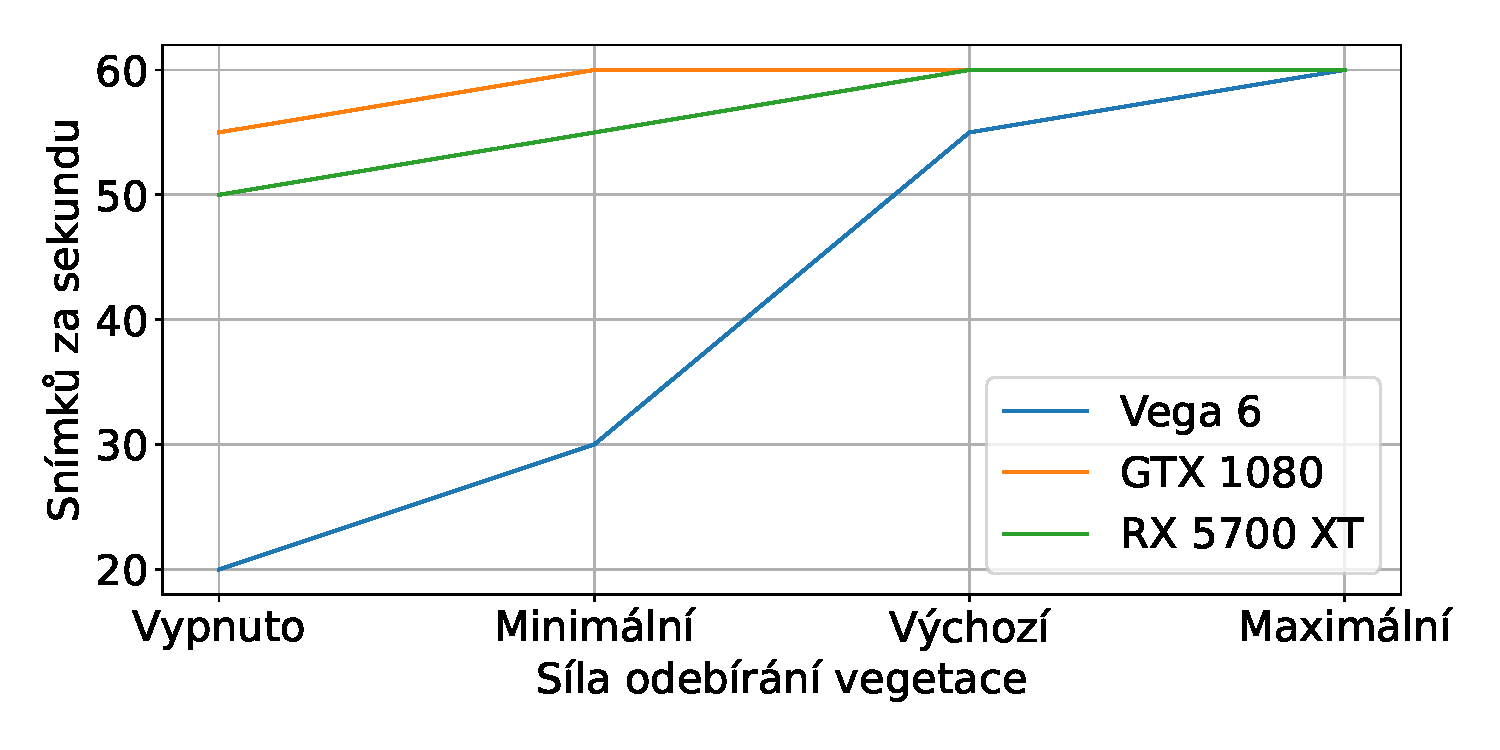
\includegraphics[width=24em]{images/impl/small_area.pdf}
	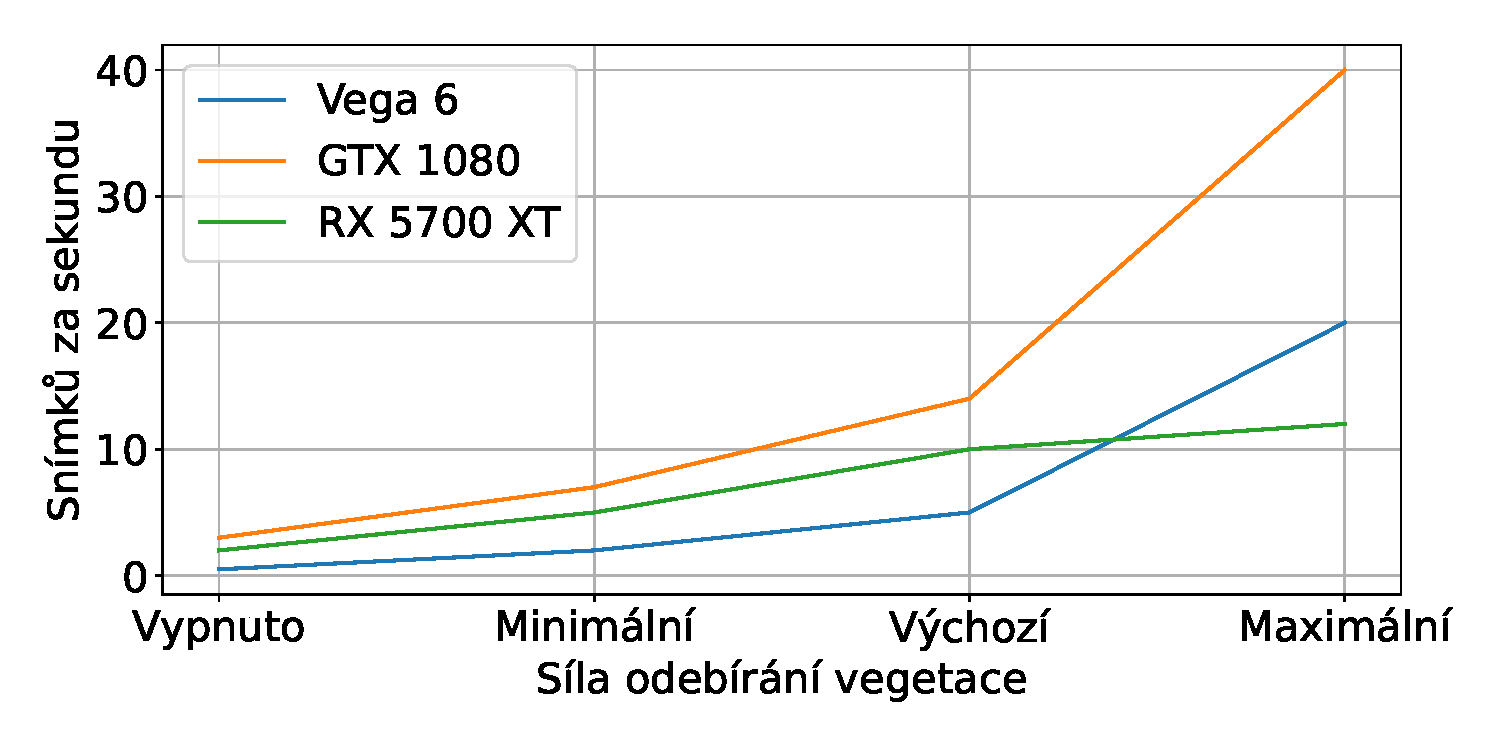
\includegraphics[width=24em]{images/impl/big_area.pdf}
	\caption[caption]{Porovnávní výkon pro malou (nahoře) a velkou (dole) oblast. Počet snímků za sekundu je limitován na 60.} 
	\label{fps-graphs}
\end{figure}

Dle grafů na obrázku \ref{fps-graphs} jde vidět, že velké oblasti jsou na notebooku i na grafické kartě \verb|RX 5700XT| špatně použitelné, a použitelné jsou pouze v~případě, že si uživatel nastaví maximální úroveň odebírání vegetace. Zároveň lze vidět chybu u~škálování s~\verb|RX 5700XT|. I~přes vysoké odebírání vegetace u~velké oblasti dosahuje pouze 12 snímků za sekundu. Grafická karta \verb|GTX 1080| zde dosahuje 40 snímků za sekundu, přestože v~moderních hrách má karta \verb|RX 5700XT| mírně vyšší výkon. Hlavní problém s~výkonem zde vzniká tím, že oblast obsahuje velmi vysoké množství vegetace, kterou některé grafické karty nestíhají zobrazovat. Na testovaném notebooku jde zároveň poznat rozdíl v~počtu snímku za sekundu i u~malých oblastí, ale zde je výkon přijatelný, pokud není odebírání vegetace úplně vypnuté. V~případě menší oblasti je hlavním zpomalením procesorový výkon, který je ve fázi generování mapy plně využit. Snímkový rozdíl u~notebooku při generování oblasti, oproti chvílím kdy je oblast již vygenerovaná, je téměř dvojnásobný. Při generování malé oblasti notebook dosahuje pouze 35 snímků za sekundu. Když je oblast již vygenerována dosahuje 60.

\section{Nedostatky v~aplikaci}
Mezi nedostatky patří několik chyb. Odrazy vodních ploch se nechovají správně. Výkon aplikace, obzvlášť v~případech, kde generování dat může trvat velmi dlouhou dobu, také není ideální. To lze zlepšit jiným přístupem generování oblasti -- místo určování správné oblasti pro každý pixel textury je možné postupně zaplňovat oblast rasterizací jednotlivých oblastí na mapě. Jako další nedostatek je uživatelské rozhraní pro vyhledávání na mapě, které nenabízí seznam výsledků, ale pouze vyhledá první možný. Dále velmi zřídka dochází k~pádům aplikace v~případě, že je generování oblasti zrušeno dřív, než je oblast dogenerována do konce. Dalším nedostatkem je generování tunelů, u~kterých se občas stane, že přestože je část cesty myšlena jako tunel, je zobrazena na povrchu místo pod.


\chapter{Závěr}
Cílem práce bylo vytvořit takovou aplikaci, která pomůže koncovému uživateli zobrazit, a tím si i lépe přestavit, jak vypadá libovolná oblast na mapě v~reálném světě. Obzvlášť důležitou částí byly různé lesní cesty, které bývají na konkurenčních aplikacích, jako je Google Earth, skryty pod vrstvou stromů. Tento cíl byl splněn.

Aplikace generuje povrch, na povrch vygeneruje několik různých textur a materiálů, dále vygeneruje několik typů vegetace, a budovy. Zobrazení je obohaceno o~několik efektů, které dělají zobrazení realističtější a hezčí.
Bylo vytvořeno video, které je ukázkou toho jak vypadají výsledky práce. To je přidáno na paměťové médium.

Při vytváření práce jsem se naučil práci s~knihovnou \verb|OpenGL| a s~knihovnou \verb|GPUEngine|. Knihovnu \verb|OpenGL| jsem doteď využil jen několikrát na velmi jednoduché projekty, a v~práci jsem se naučil pokročilejší zobrazovací techniky a metody. Dále jsem si v~práci lépe vyzkoušel asynchroní programování, obzvlášť pak s~využitím knihovny \verb|OpenMP|.

Aplikace byla původně navržena tak, aby měla co nejméně dependencí, ale při implementaci se ukázalo že nejlepším způsobem bylo využít na některé věci knihovny s~ohledem na čas a náročnost projektu.

Aplikace byla několikrát upravena podle uživatelského testování. Hlavní změny přišly v~uživatelském rozhraní a v~ovládání aplikace, které uživatelům nevyhovovavly. Většina uživatelů ale instinktivně zjistila, jak se v~generovaném modelu pohybuje s~kamerou, a jak se vybírá na mapě oblast, která se bude generovat.

Jako další rozšíření práce je kromě vyřešení aktuálních nedostatků přidání další funkcionality. Další funkcionalitou může být například možnost uložit si generovanou oblast, uložit si pouze metadata k~libovolné velké oblasti, ze které by aplikace mohla získávat data i bez přístupu k~internetu. Dále bych chtěl přidat detekci více různých oblastí (hlavně ledovce a sníh) a přidání různých typů oblohy podle toho, kde je oblast generována. Dalším možným rozšířením je přepsání aplikace tak, aby byla zkompilovatelná do technologoií jako je \verb|wasm| a zobrazování do \verb|WebGL|, tak aby mohla aplikace být použita například na webových stránkách.



%===============================================================================

  \fi
  
  % Kompilace po částech (viz výše, nutno odkomentovat)
  % Compilation piecewise (see above, it is necessary to uncomment it)
  %\subfile{projekt-01-uvod-introduction}
  % ...
  %\subfile{chapters/projekt-05-conclusion}


  % Pouzita literatura / Bibliography
  % ----------------------------------------------
\ifslovak
  \makeatletter
  \def\@openbib@code{\addcontentsline{toc}{chapter}{Literatúra}}
  \makeatother
  \bibliographystyle{bib-styles/Pysny/skplain}
\else
  \ifczech
    \makeatletter
    \def\@openbib@code{\addcontentsline{toc}{chapter}{Literatura}}
    \makeatother
    \bibliographystyle{bib-styles/Pysny/czplain}
  \else 
    \makeatletter
    \def\@openbib@code{\addcontentsline{toc}{chapter}{Bibliography}}
    \makeatother
    \bibliographystyle{bib-styles/Pysny/enplain}
  %  \bibliographystyle{alpha}
  \fi
\fi
  \begin{flushleft}
  \bibliography{projekt-20-literatura-bibliography}
  \end{flushleft}

  % vynechani stranky v oboustrannem rezimu
  % Skip the page in the two-sided mode
  \iftwoside
    \cleardoublepage
  \fi

  % Prilohy / Appendices
  % ---------------------------------------------
  \appendix
\ifczech
  \renewcommand{\appendixpagename}{Přílohy}
  \renewcommand{\appendixtocname}{Přílohy}
  \renewcommand{\appendixname}{Příloha}
\fi
\ifslovak
  \renewcommand{\appendixpagename}{Prílohy}
  \renewcommand{\appendixtocname}{Prílohy}
  \renewcommand{\appendixname}{Príloha}
\fi
%  \appendixpage

% vynechani stranky v oboustrannem rezimu
% Skip the page in the two-sided mode
%\iftwoside
%  \cleardoublepage
%\fi
  
\ifslovak
%  \section*{Zoznam príloh}
%  \addcontentsline{toc}{section}{Zoznam príloh}
\else
  \ifczech
%    \section*{Seznam příloh}
%    \addcontentsline{toc}{section}{Seznam příloh}
  \else
%    \section*{List of Appendices}
%    \addcontentsline{toc}{section}{List of Appendices}
  \fi
\fi
  \startcontents[chapters]
  \setlength{\parskip}{0pt} 
  % seznam příloh / list of appendices
  % \printcontents[chapters]{l}{0}{\setcounter{tocdepth}{2}}
  
  \ifODSAZ
    \setlength{\parskip}{0.5\bigskipamount}
  \else
    \setlength{\parskip}{0pt}
  \fi
  
  % vynechani stranky v oboustrannem rezimu
  \iftwoside
    \cleardoublepage
  \fi
  
  % Přílohy / Appendices
  \ifenglish
    \input{projekt-30-prilohy-appendices-en}
  \else
    % Tento soubor nahraďte vlastním souborem s přílohami (nadpisy níže jsou pouze pro příklad)



\chapter{Obrázky s vygenerovanou mapou}
\begin{figure}[H]
	\centering
	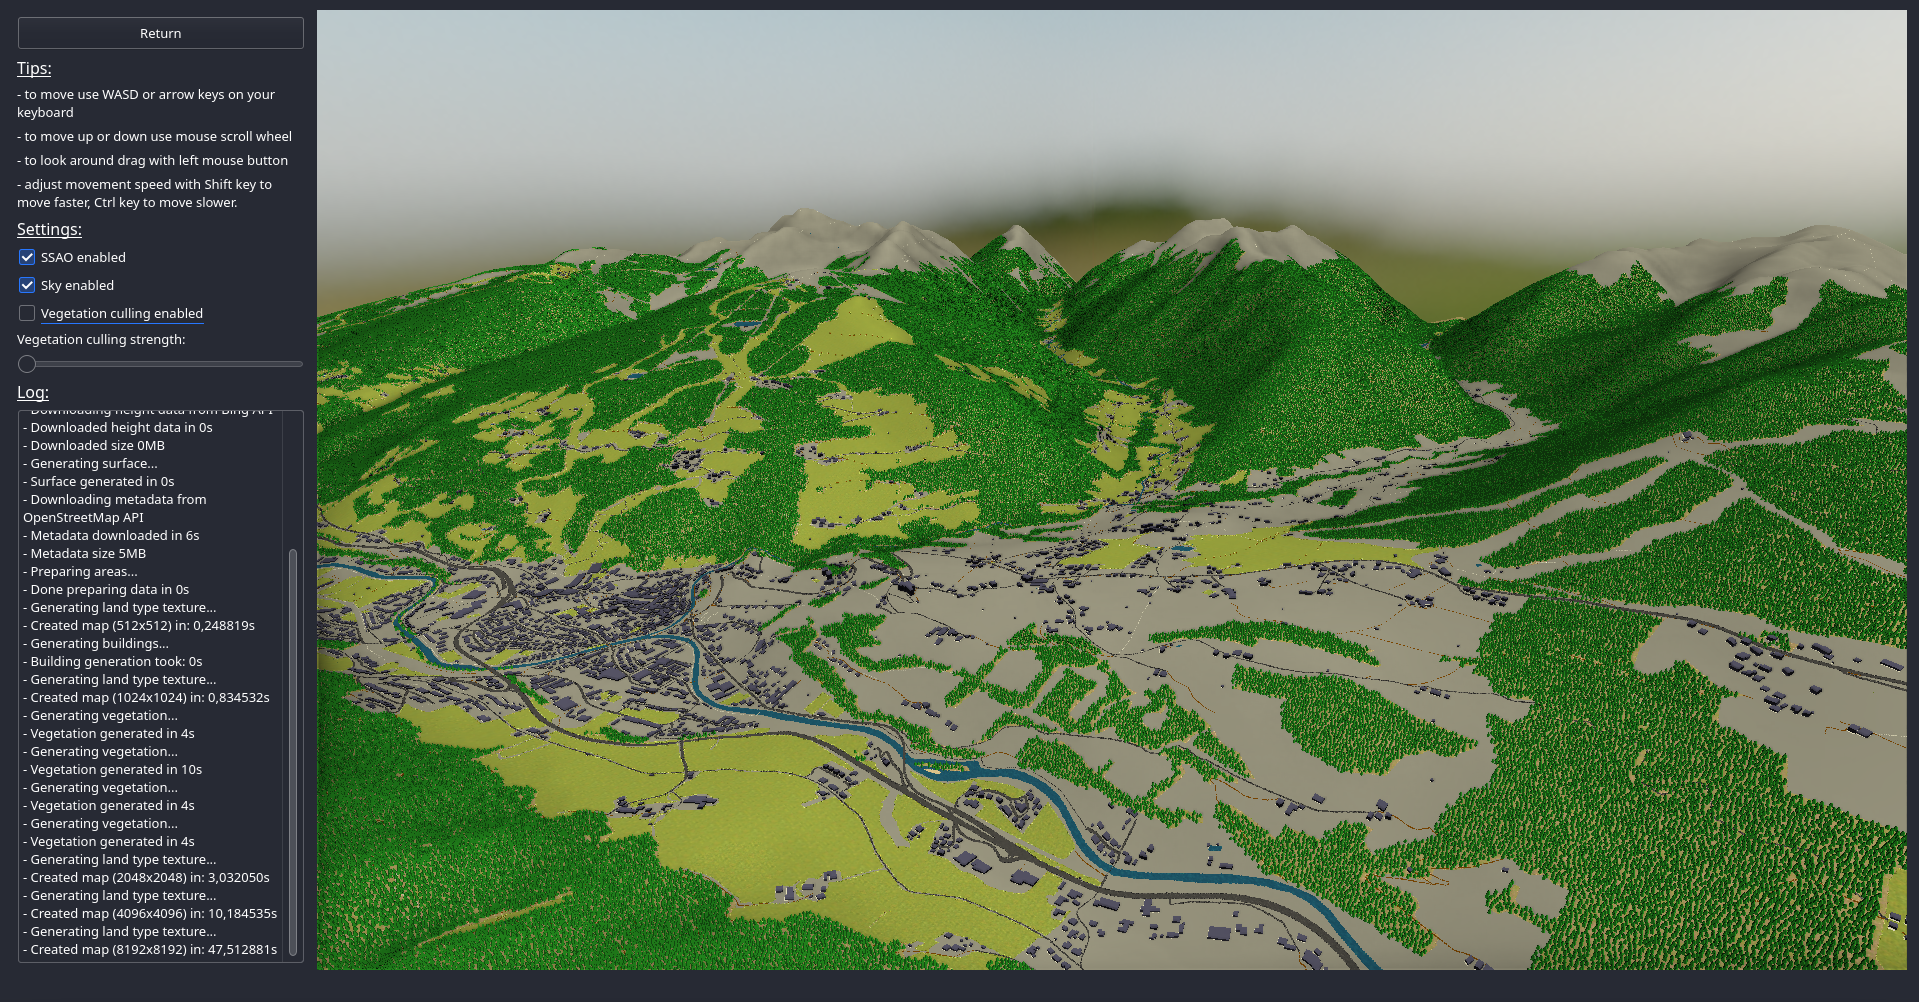
\includegraphics[width=40em]{images/results/schladming.png}
	\caption[caption]{Hornatá oblast v Rakousku okolo města Schladming.} 
	\label{img-austria}
\end{figure}

\begin{figure}[H]
	\centering
	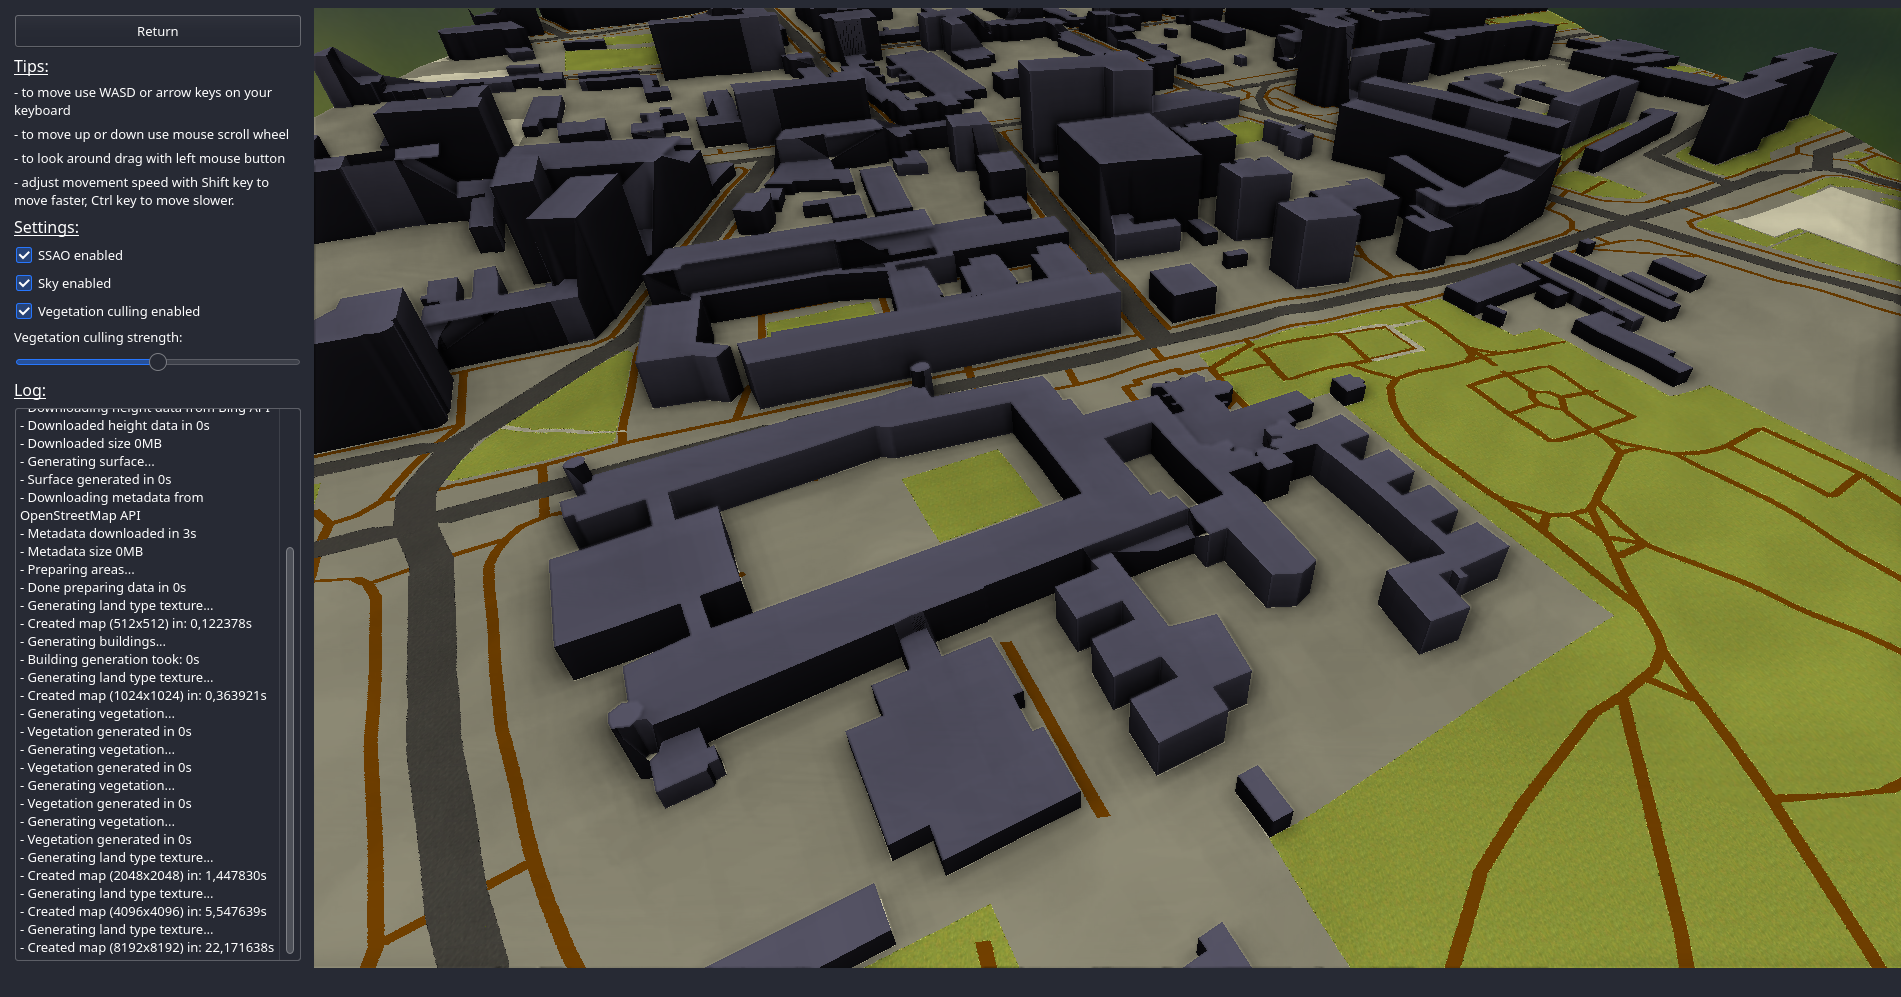
\includegraphics[width=39em]{images/results/faculty.png}
	\caption[caption]{Přiblížený pohled na VUT FIT ze západu.} 
	\label{img-fit}
\end{figure}


\begin{figure}[H]
	\centering
	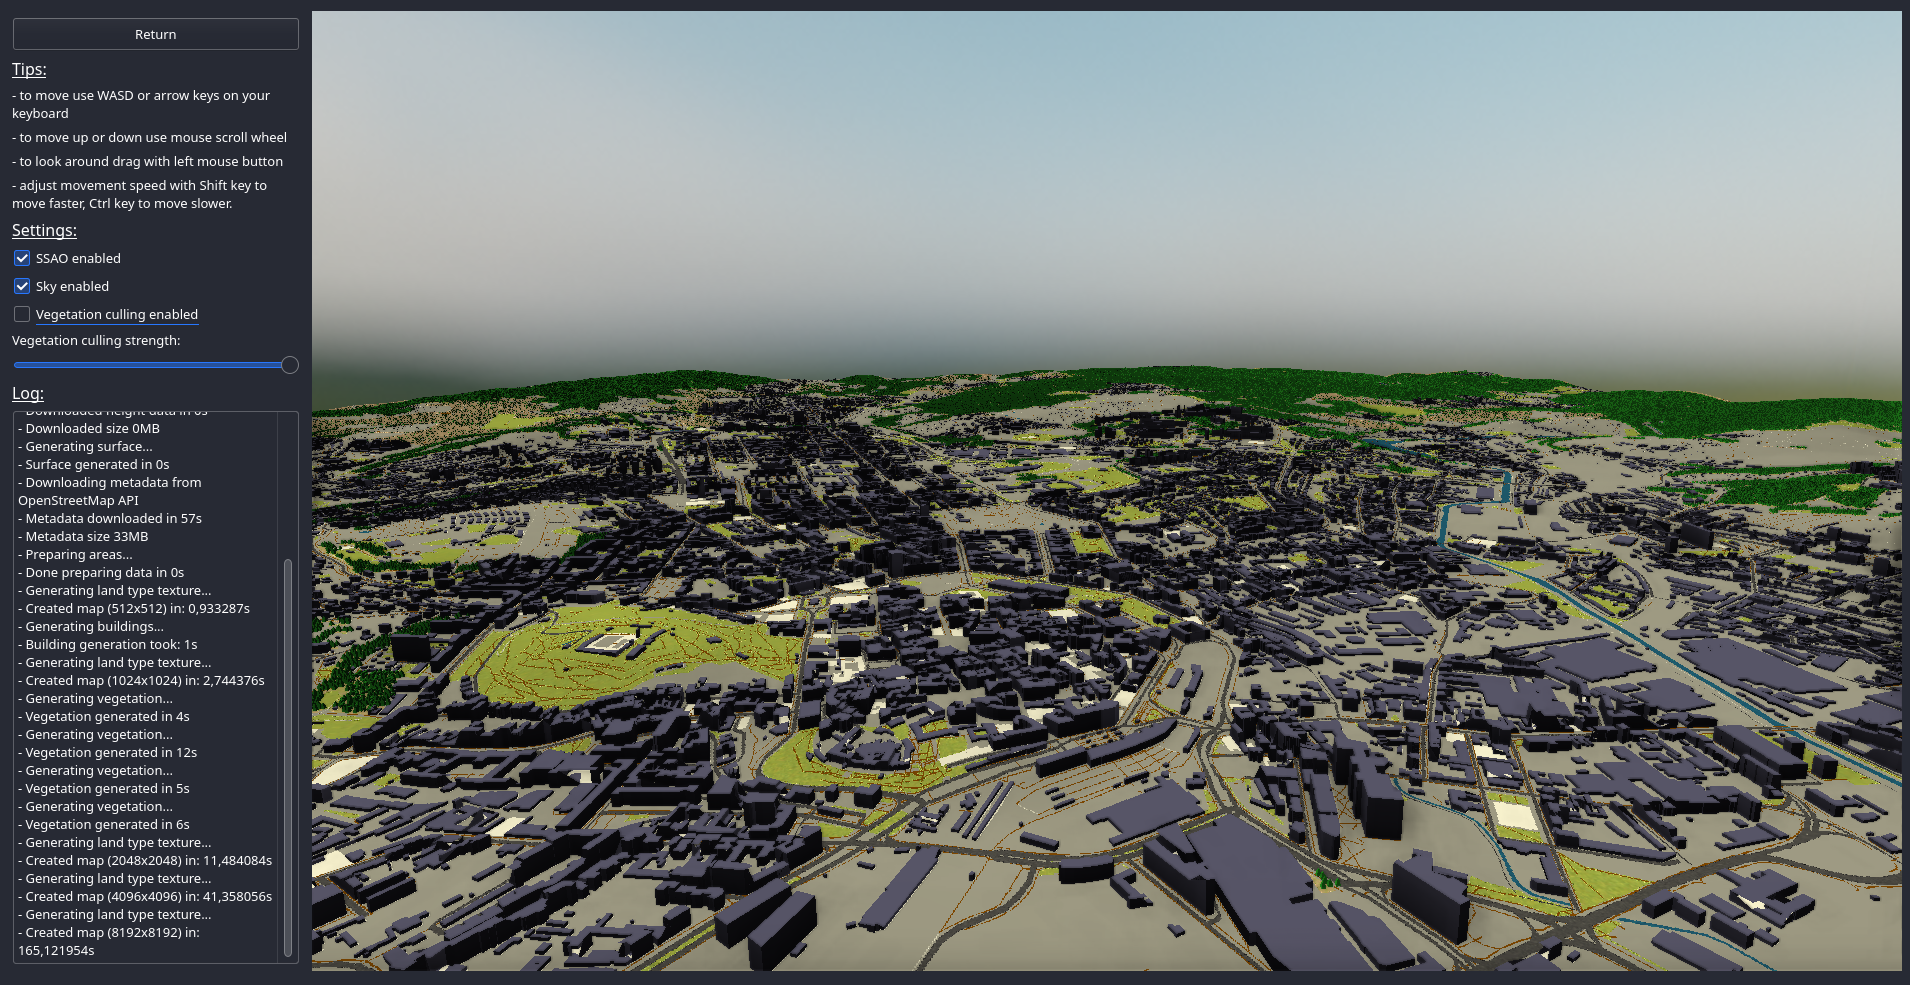
\includegraphics[width=39em]{images/results/brno.png}
	\caption[caption]{Pohled na centrum města Brna a dále na sever.} 
	\label{img-brno}
\end{figure}


\chapter{Konfigurační soubor}
Konfigurační soubor musí být aplikaci při spuštění přiřazen přes argument v příkazové řádce. Jeho formát je následující:
\begin{lstlisting}
{
  "keys":[
      {
        "service": "<name>",
        "key": "<value>"
      }
    ], "options":{
    "terrainResolution": <number>,
    "minTextureResolution": <number>,
    "maxTextureResolution": <number>,
    "textureResolutionStep": <number>,
    "generateVegetationAt": <number>,
    "randomSeed": <number>
  }

}

\end{lstlisting}
\begin{itemize}
    \item \textbf{keys} -- seznamů klíčů k autorizace na různé API
    \begin{itemize}
        \item \textbf{service} -- název služby, ke které patří klíč
        \item \textbf{key} -- hodnota klíče
    \end{itemize}
    \item \textbf{options} -- nastavení generátoru mapy
    \begin{itemize}
         \item \textbf{terrainResolution} -- rozlišení generovaného povrchu
    \item \textbf{minTextureResolution} -- minimální rozlišení textury s metadaty pro oblast
    \item \textbf{maxTextureResolution} -- maximální rozlišení textury s metadaty pro oblast
    \item \textbf{textureResolutionStep} -- násobič o kolik se změní každé další generování textury
    \item \textbf{generateVegetationAt} -- hodnota rozlišení textury s metadaty, při které bude vygenerována vegetace
    \item \textbf{randomSeed} -- vstup pro náhodné generátory čísel
    \end{itemize}
\end{itemize}


\chapter{Obsah paměťového média}

Paměťové médium ve formě CD má následující strukturu:

\begin{itemize}
    \item \textbf{src/} -- složka, obsahující veškeré zdrojové soubory práce
    \item \textbf{bin/} -- sestavené binární soubory pro systém Manjaro Linux
    \item \textbf{text/} -- zdrojové soubory k textové části práce
    \item \textbf{CMakeLists.txt} -- soubor, sloužící k překladu projektu pomocí programu cmake
    \item \textbf{Makefile} -- soubor, který využívá program make k tomu, aby vytvořil všechny potřebané složky a pomocí volání cmake sestavil celou aplikaci
    \item \textbf{config.json} -- ukázkový konfigurační souboru aplikace.
    \item \textbf{video.mp4} -- výsledek práce v podobě videa
    \item \textbf{thesis.pdf} -- tento text práce v zkompilovaném digitálním formátu
    \item \textbf{doc.pdf} -- návod ke kompilaci a použití projektu
\end{itemize}
  \fi
  
  % Kompilace po částech (viz výše, nutno odkomentovat)
  % Compilation piecewise (see above, it is necessary to uncomment it)
  %\subfile{projekt-30-prilohy-appendices}
  
\end{document}
